
%% Waves Questions used on the
%% NYSED Physics Regents Examination
%%--------------------------------------------------

%% this section contains 161 problems


%% Section June2016
%%--------------------
\element{nysed}{
\begin{question}{June2016-Q21}
    The time required to produce one cycle of a wave is known as the wave's:
    \begin{multicols}{2}
    \begin{choices}
        \wrongchoice{amplitude}
        \wrongchoice{frequency}
      \correctchoice{period}
        \wrongchoice{wavelength}
    \end{choices}
    \end{multicols}
\end{question}
}


%% Section June2015
%%--------------------
\element{nysed}{
\begin{question}{June2015-Q24}
    A student produces a wave in a long spring by vibrating its end.
    As the frequency of the vibration is doubled,
        the wavelength in the spring is:
    \begin{multicols}{2}
    \begin{choices}
        \wrongchoice{quartered}
      \correctchoice{halved}
        \wrongchoice{unchanged}
        \wrongchoice{doubled}
    \end{choices}
    \end{multicols}
\end{question}
}

\element{nysed}{
\begin{question}{June2015-Q25}
    Which two points on the wave shown in the diagram below are in phase with each other?
    \begin{center}
    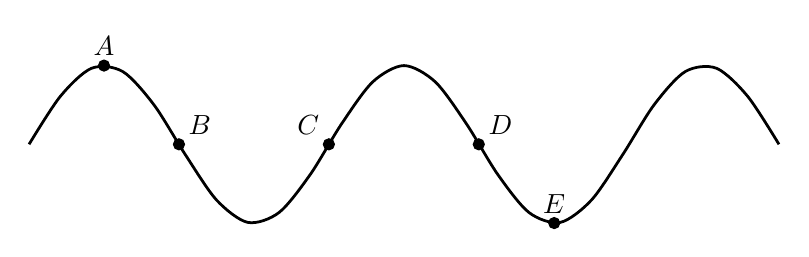
\begin{tikzpicture}[x=0.05\textwidth]
        %% Graph
        \draw[domain=0:5*pi,smooth,line width=1pt] plot (\x, {sin(\x r)});
        %% Labels
        \draw[fill] (1.57,1) circle (2pt) node[anchor=south] {$A$};
        \draw[fill] (3.14,0) circle (2pt) node[anchor=south west] {$B$};
        \draw[fill] (6.28,0) circle (2pt) node[anchor=south east] {$C$};
        \draw[fill] (9.42,0) circle (2pt) node[anchor=south west] {$D$};
        \draw[fill] (11.0,-1) circle (2pt) node[anchor=south] {$E$};
    \end{tikzpicture}
    \end{center}
    \begin{multicols}{2}
    \begin{choices}
        \wrongchoice{$A$ and $B$}
        \wrongchoice{$A$ and $E$}
        \wrongchoice{$B$ and $C$}
      \correctchoice{$B$ and $D$}
    \end{choices}
    \end{multicols}
\end{question}
}

\element{nysed}{
\begin{question}{June2015-Q26}
    As a longitudinal wave moves through a medium,
        the particles of the medium:
    \begin{choices}
      \correctchoice{vibrate parallel to the direction of the wave's propagation.}
        \wrongchoice{vibrate perpendicular to the direction of the wave's propagation.}
        \wrongchoice{are transferred in the direction of the wave’s motion, only.}
        \wrongchoice{are stationary.}
    \end{choices}
\end{question}
}

\element{nysed}{
\begin{question}{June2015-Q27}
    Wind blowing across suspended power lines may cause the power lines to vibrate at their natural frequency.
    This often produces audible sound waves.
    This phenomenon, often called an Aeolian harp,
        is an example of:
    \begin{multicols}{2}
    \begin{choices}
        \wrongchoice{diffraction}
        \wrongchoice{the Doppler effect}
        \wrongchoice{refraction}
      \correctchoice{resonance}
    \end{choices}
    \end{multicols}
\end{question}
}

\element{nysed}{
\begin{question}{June2015-Q35}
    Two pulses approach each other in the same medium.
    The diagram below represents the displacements caused by each pulse.
    \begin{center}
    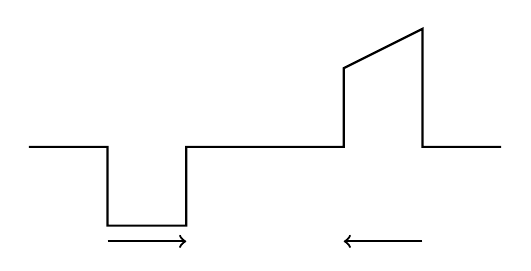
\begin{tikzpicture}
        \draw[thick] (-3,0) -- (-2,0) -- (-2,-1) -- (-1,-1) -- (-1,0) --
                     (+1,0) -- (+1,1) -- (+2,1.5) -- (+2,0) -- (+3,0);
        \draw[thick,->] (-2,-1.2) -- (-1,-1.2);
        \draw[thick,->] (+2,-1.2) -- (+1,-1.2);
    \end{tikzpicture}
    \end{center}
    Which diagram best represents the resultant displacement of the medium as the pulses pass through each other?
    \begin{multicols}{2}
    \begin{choices}
        \AMCboxDimensions{down=-0.5cm}
        \wrongchoice{
            \begin{tikzpicture}
                \draw[white] (-1.5,-0.5) rectangle (1.5,3.0);
                \draw[thick] (-1.5,0) -- (1.5,0);
            \end{tikzpicture}
        }
        \correctchoice{
            \begin{tikzpicture}
                \draw[white] (-1.5,-0.5) rectangle (1.5,3.0);
                \draw[thick] (-1.5,0) -- (-0.5,0) -- (0.5,0.5) -- (0.5,0) --  (1.5,0);
            \end{tikzpicture}
        }
        \wrongchoice{
            \begin{tikzpicture}
                \draw[white] (-1.5,-0.5) rectangle (1.5,3.0);
                \draw[thick] (-1.5,0) -- (-0.5,0) -- (-0.5,2.0) -- (0.5,2.5) -- (0.5,0) --  (1.5,0);
            \end{tikzpicture}
        }
        \wrongchoice{
            \begin{tikzpicture}
                \draw[white] (-1.5,-0.5) rectangle (1.5,3.0);
                \draw[thick] (-1.5,0) -- (-0.5,0) -- (0.5,-0.5) -- (0.5,0) --  (1.5,0);
            \end{tikzpicture}
        }
    \end{choices}
    \end{multicols}
\end{question}
}

\element{nysed}{
\begin{question}{June2015-Q49}
    The diagram below shows waves $A$ and $B$ in the same medium.
    %Wave $A$ and $B$ are represented as a dashed and solid line.
    \begin{center}
    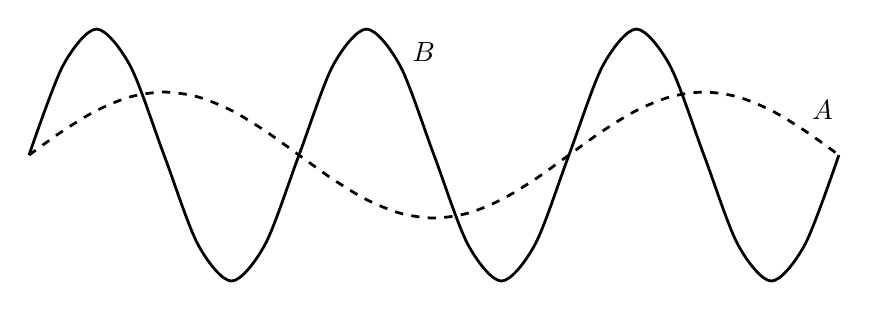
\begin{tikzpicture}[x=0.045\textwidth,yscale=0.8]
        %% Graph
        \draw[domain=0:6*pi,smooth,line width=1pt] plot (\x, {2.0*sin(\x r)});
        \draw[domain=0:6*pi,dashed,smooth,line width=1pt] plot (\x, {sin(0.5*\x r)});
        %% Labels
        \node[anchor=south west] at (8.7,{2.0*sin(8.7 r)})  {$B$};
        \node[anchor=south west] at (18,{sin(0.5*18 r)})  {$A$};
    \end{tikzpicture}
    \end{center}
    Compared to wave $A$, wave $B$ has:
    \begin{choices}
        \wrongchoice{twice the amplitude and twice the wavelength.}
      \correctchoice{twice the amplitude and half the wavelength.}
        \wrongchoice{the same amplitude and half the wavelength.}
        \wrongchoice{half the amplitude and the same wavelength.}
    \end{choices}
\end{question}
}


%% Section June2014
%%--------------------
\element{nysed}{
\begin{question}{June2014-Q17}
    Transverse waves are to radio waves as longitudinal waves are to:
    \begin{multicols}{2}
    \begin{choices}
      \correctchoice{sound waves}
        \wrongchoice{light waves}
        \wrongchoice{microwaves}
        \wrongchoice{ultraviolet waves}
    \end{choices}
    \end{multicols}
\end{question}
}

\element{nysed}{
\begin{question}{June2014-Q25}
    The diagram below represents two identical pulses approaching each other in a uniform medium.
    \begin{center}
    \begin{tikzpicture}
        \begin{axis}[
            clip=false,
            axis y line=left,
            axis x line=center,
            axis line style={->},
            xlabel=\empty,
            xtick=\empty,
            ylabel={displacement},
            y unit=\si{\centi\meter},
            ytick={-6,-3,0,3,6},
            xmin=0,xmax=10,
            ymin=-7,ymax=7,
            grid=major,
            width=0.95\columnwidth,
            height=0.618\columnwidth,
            very thin,
        ]
        \addplot[very thick,domain=0:2]{0};
        \addplot[very thick,domain=4:6]{0};
        \addplot[very thick,domain=8:10]{0};
        %% Waves
        \addplot[very thick,domain=2:4]{-3*(x-2)*(x-4)};
        \addplot[very thick,domain=6:8]{-3*(x-6)*(x-8)};
        %% Arrows
        \draw[very thick,->] (axis cs:2,4) -- (axis cs:4,4);
        \draw[very thick,->] (axis cs:8,4) -- (axis cs:6,4);
        %% Labels
        \node[at={(axis cs:3,4)},above=3pt] {Pulse $A$};
        \node[at={(axis cs:7,4)},above=3pt] {Pulse $B$};
        \end{axis}
    \end{tikzpicture}
    \end{center}
    As the pulses meet and are superposed,
        the maximum displacement of the medium is:
    \begin{multicols}{2}
    \begin{choices}
      \correctchoice{\SI{6}{\centi\meter}}
        \wrongchoice{\SI{0}{\centi\meter}}
        \wrongchoice{\SI{3}{\centi\meter}}
        \wrongchoice{\SI{-6}{\centi\meter}}
    \end{choices}
    \end{multicols}
\end{question}
}

\element{nysed}{
\begin{question}{June2014-Q34}
    The diagram below represents two waves, $A$ and $B$,
        traveling through the same uniform medium.
    \begin{center}
    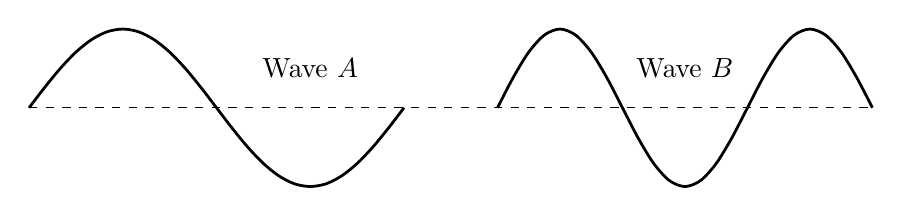
\begin{tikzpicture}[x=0.0625\textwidth]
        %% Graph
        \draw[domain=0:2*pi,smooth,line width=1pt] plot (\x, {sin(\x r)});
        \draw[domain=0:2*pi,smooth,line width=1pt] plot (\x+7.85, {sin(1.5*\x r)});
        \draw[dashed] (0,0) -- (14.13,0);
        %% Labels
        \node[anchor=center] at (4.71,0.5) {Wave $A$};
        \node[anchor=center] at (10.99,0.5) {Wave $B$};
    \end{tikzpicture}
    \end{center}
    Which characteristic is the same for both waves?
    \begin{multicols}{2}
    \begin{choices}
      \correctchoice{amplitude}
        \wrongchoice{period}
        \wrongchoice{wavelength}
        \wrongchoice{frequency}
    \end{choices}
    \end{multicols}
\end{question}
}

\element{nysed}{
\begin{question}{June2014-Q35}
    The diagram below shows a periodic wave.
    \begin{center}
    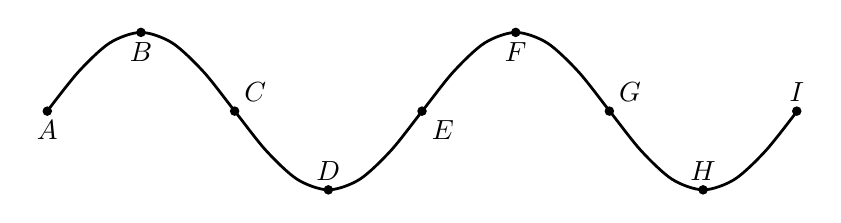
\begin{tikzpicture}[x=0.0625\textwidth]
        %% Graph
        \draw[domain=0:4*pi,smooth,line width=1pt] plot (\x, {sin(\x r)});
        %% Labels
        \node[anchor=north]     at (0,0)    {$A$};
            \draw[fill] (0,0) circle [radius=1.5pt];
        \node[anchor=north]     at (1.57,1) {$B$};
            \draw[fill] (1.57,1) circle [radius=1.5pt];
        \node[anchor=south west]at (3.14,0) {$C$};
            \draw[fill] (3.14,0) circle [radius=1.5pt];
        \node[anchor=south]     at (4.71,-1) {$D$};
            \draw[fill] (4.71,-1) circle [radius=1.5pt];
        \node[anchor=north west]at (6.28,0){$E$};
            \draw[fill] (6.28,0) circle [radius=1.5pt];
        \node[anchor=north]     at (7.85,1){$F$};
            \draw[fill] (7.85,1) circle [radius=1.5pt];
        \node[anchor=south west]at (9.42,0){$G$};
            \draw[fill] (9.42,0) circle [radius=1.5pt];
        \node[anchor=south]     at (10.99,-1){$H$};
            \draw[fill] (10.99,-1) circle [radius=1.5pt];
        \node[anchor=south]     at (12.56,0) {$I$};
            \draw[fill] (12.56,0) circle [radius=1.5pt];
    \end{tikzpicture}
    \end{center}
    Which two points on the wave are \ang{180} out of phase?
    \begin{multicols}{2}
    \begin{choices}
      \correctchoice{$A$ and $C$}
        \wrongchoice{$B$ and $E$}
        \wrongchoice{$F$ and $G$}
        \wrongchoice{$D$ and $H$}
    \end{choices}
    \end{multicols}
\end{question}
}


%% Section June2013
%%--------------------
\element{nysed}{
\begin{question}{June2013-Q20}
    What is the speed of light ($f=\SI{5.09e14}{\hertz}$) in ethyl alcohol?
    \begin{multicols}{2}
    \begin{choices}
        \wrongchoice{\SI{4.53e-9}{\meter\per\second}}
        \wrongchoice{\SI{2.43e2}{\meter\per\second}}
        \wrongchoice{\SI{1.24e8}{\meter\per\second}}
      \correctchoice{\SI{2.21e8}{\meter\per\second}}
    \end{choices}
    \end{multicols}
\end{question}
}

\element{nysed}{
\begin{question}{June2013-Q22}
    The diagram below represents a periodic wave.
    \begin{center}
    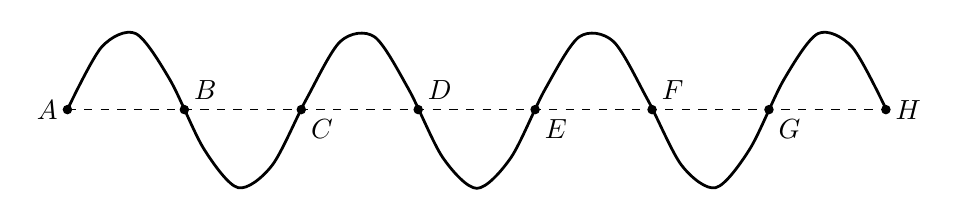
\begin{tikzpicture}[x=0.039\textwidth]
        %% Graph
        \draw[domain=0:7*pi,smooth,line width=1pt] plot (\x, {sin(\x r)});
        \draw[dashed] (0,0) -- (21.98,0);
        %% Circles and Labels
        \draw[fill] (0,0) circle [radius=1.5pt]
            node[anchor=east] {$A$};
        \draw[fill] (3.14,0)  circle [radius=1.5pt]
            node[anchor=south west] {$B$};
        \draw[fill] (6.28,0)  circle [radius=1.5pt]
            node[anchor=north west] {$C$};
        \draw[fill] (9.42,0) circle [radius=1.5pt]
            node[anchor=south west] {$D$};
        \draw[fill] (12.56,0) circle [radius=1.5pt]
            node[anchor=north west] {$E$};
        \draw[fill] (15.7,0) circle [radius=1.5pt]
            node[anchor=south west] {$F$};
        \draw[fill] (18.84,0) circle [radius=1.5pt]
            node[anchor=north west] {$G$};
        \draw[fill] (21.98,0) circle [radius=1.5pt]
            node[anchor=west] {$H$};
    \end{tikzpicture}
    \end{center}
    Which two points on the wave are out of phase?
    \begin{multicols}{2}
    \begin{choices}
        \wrongchoice{$A$ and $C$}
        \wrongchoice{$B$ and $F$}
        \wrongchoice{$C$ and $E$}
      \correctchoice{$D$ and $G$}
    \end{choices}
    \end{multicols}
\end{question}
}

\element{nysed}{
\begin{question}{June2013-Q24}
    A distance of \SI{1.0e-2}{\meter} separates successive crests
        of a periodic wave produced in a shallow tank of water.
    If a crest passes a point in the tank every \SI{4.0e-1}{\second},
        what is the speed of this wave?
    \begin{multicols}{2}
    \begin{choices}
        \wrongchoice{\SI{2.5e-4}{\meter\per\second}}
        \wrongchoice{\SI{4.0e-3}{\meter\per\second}}
      \correctchoice{\SI{2.5e-2}{\meter\per\second}}
        \wrongchoice{\SI{4.0e-1}{\meter\per\second}}
    \end{choices}
    \end{multicols}
\end{question}
}

\element{nysed}{
\begin{question}{June2013-Q48}
    The diagram below shows two waves traveling toward each other
        at equal speed in a uniform medium.
    \begin{center}
    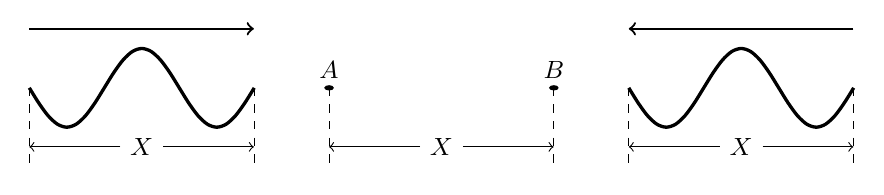
\begin{tikzpicture}[x=0.025\textwidth,yscale=0.5,font=\small]
        %% Wave A
        \draw[domain=0:3*pi,smooth,very thick] plot (\x, {-1*sin(\x r)});
            \draw[thick,->] (0,1.5)   to (9.41,1.5);
        \draw[dashed] (0,0)     to (0,-2);
        \draw[dashed] (9.42,0)  to (9.42,-2);
        \node[anchor=center] (XA) at (4.71,-1.5) {$X$};
            \draw[->] (XA) -- (0,-1.5);
            \draw[->] (XA) -- (9.41,-1.5);
        %% Middle (offset 12.56)
        \node[anchor=south]     at (12.56,0) {$A$};
            \draw[fill] (12.56,0) circle [radius=1.5pt];
        \node[anchor=south]     at (21.98,0) {$B$};
            \draw[fill] (21.98,0) circle [radius=1.5pt];
        \draw[dashed] (12.56,0) -- (12.56,-2);
        \draw[dashed] (21.98,0) -- (21.98,-2);
        \node[anchor=center] (XM) at (17.27,-1.5) {$X$};
            \draw[->] (XM) -- (12.56,-1.5);
            \draw[->] (XM) -- (21.97,-1.5);
        %% Wave B (offset 25.12)
        \draw[domain=0:3*pi,smooth,very thick] plot (\x+25.12, {-1*sin(\x r)});
            \draw[thick,->] (34.53,1.5) -- (25.12,1.5);
        \draw[dashed] (25.12,0)  to (25.12,-2);
        \draw[dashed] (34.54,0)  to (34.54,-2);
        \node[anchor=center] (XB) at (29.83,-1.5) {$X$};
            \draw[->] (XB) -- (25.12,-1.5);
            \draw[->] (XB) -- (34.53,-1.5);
    \end{tikzpicture}
    \end{center}
    When both waves are in the region between points $A$ and $B$,
        they will undergo
    \begin{choices}
        \wrongchoice{diffraction}
        \wrongchoice{the Doppler effect}
        \wrongchoice{destructive interference}
      \correctchoice{constructive interference}
    \end{choices}
\end{question}
}

\element{nysed}{
\begin{question}{June2013-Q49}
    The diagram below shows a series of straight wave fronts produced
        in a shallow tank of water approaching a small opening in
        a barrier.
    \begin{center}
    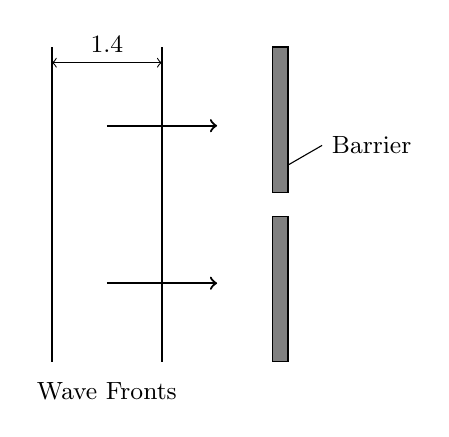
\begin{tikzpicture}[font=\small]
        %% Incoming
        \foreach \x in {0,1.40}
            \draw[thick] (\x,-2) -- (\x,2);
        \draw[thick,->] (0.7,1.0) -- (2.1,1.0);
        \draw[thick,->] (0.7,-1.0) -- (2.1,-1.0);
        %% Barrier
        \draw[fill=black!50!white] (2.8,0.15) rectangle (3.0,2);
        \draw[fill=black!50!white] (2.8,-0.15) rectangle (3.0,-2);
        \draw (3.0,0.5) -- ++ (30:0.5cm)
            node[pos=1.0,anchor=west] {Barrier};
        %% Labels
        \draw[<->] (0,1.8) -- (1.4,1.8)
            node[anchor=south,pos=0.5] {\SI{1.4}{\centi\meter}};
        \node[anchor=north,yshift=-4pt] at (0.7,-2.0) {Wave Fronts};
    \end{tikzpicture}
    \end{center}
    Which diagram represents the appearance of the wave fronts
        after passing through the opening in the barrier?
    \begin{multicols}{2}
    \begin{choices}
        \AMCboxDimensions{down=-2.0cm}
        \wrongchoice{
            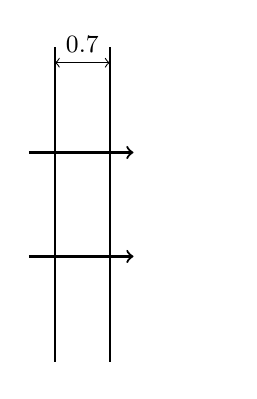
\begin{tikzpicture}[font=\small]
                \draw[white] (-0.33,-2.1) rectangle (2.2,2.1);
                \foreach \x in {0,0.7}
                    \draw[thick] (\x,-2) -- (\x,2);
                \foreach \y in {-0.66,0.66}
                    \draw[thick,->] (-0.33,\y) -- (1.0,\y);
                \draw[<->] (0,1.8) -- (0.7,1.8)
                    node[pos=0.5,anchor=south] {\num{0.7}}
                    node[pos=0.5,anchor=north] {\si{\centi\meter}};
            \end{tikzpicture}
        }
        \wrongchoice{
            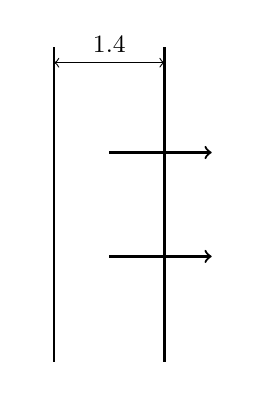
\begin{tikzpicture}[font=\small]
                \draw[white] (-0.33,-2.1) rectangle (2.2,2.1);
                \foreach \x in {0,1.4}
                    \draw[thick] (\x,-2) -- (\x,2);
                \foreach \y in {-0.66,0.66}
                    \draw[thick,->] (0.7,\y) -- (2.0,\y);
                \draw[<->] (0,1.8) -- (1.4,1.8)
                    node[pos=0.5,anchor=south] {\SI{1.4}{\centi\meter}};
            \end{tikzpicture}
        }
        %% Arcs
        \wrongchoice{
            \begin{tikzpicture}[font=\small]
                \draw[white] (-0.33,-2.1) rectangle (2.2,2.1);
                \foreach \x in {0.35,1.05}
                    \draw[thick] (270:\x) arc (-90:90:\x);
                \foreach \d in {45,315}
                    \draw[thick,->] (\d:0.70) -- ++ (\d:0.7);
                \draw[<->] (0:0.35) -- (0:1.05)
                    node[pos=0.5,anchor=south] {\num{0.7}}
                    node[pos=0.5,anchor=north] {\si{\centi\meter}};
            \end{tikzpicture}
        }
        \correctchoice{
            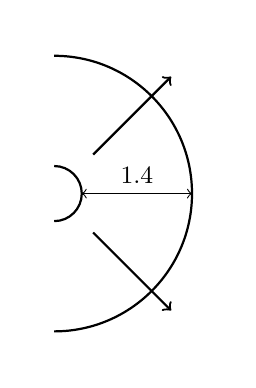
\begin{tikzpicture}[font=\small]
                \draw[white] (-0.33,-2.1) rectangle (2.2,2.1);
                \foreach \x in {0.35,1.75}
                    \draw[thick] (270:\x) arc (-90:90:\x);
                \foreach \d in {45,315}
                    \draw[thick,->] (\d:0.70) -- ++ (\d:1.4);
                \draw[<->] (0:0.35) -- (0:1.75)
                    node[pos=0.5,anchor=south] {\SI{1.4}{\centi\meter}};
            \end{tikzpicture}
        }
    \end{choices}
    \end{multicols}
\end{question}
}


%% Section June2012
%%--------------------
\element{nysed}{
\begin{question}{June2012-Q21}
    The wavelength of a wave doubles as it travels from medium $A$ into medium $B$.
    Compared to the wave in medium $A$,
        the wave in medium $B$ has:
    \begin{choices}
        \wrongchoice{half the speed}
      \correctchoice{twice the speed}
        \wrongchoice{half the frequency}
        \wrongchoice{twice the frequency}
    \end{choices}
\end{question}
}

\element{nysed}{
\begin{question}{June2012-Q29}
    What is characteristic of both sound waves and electromagnetic waves?
    \begin{choices}
        \wrongchoice{They require a medium.}
      \correctchoice{They transfer energy.}
        \wrongchoice{They are mechanical waves.}
        \wrongchoice{They are longitudinal waves.}
    \end{choices}
\end{question}
}

\element{nysed}{
\begin{question}{June2012-Q34}
    While sitting in a boat, a fisherman observes that two complete waves pass by his position every \SI{4}{\second}.
    What is the period of these waves?
    \begin{multicols}{4}
    \begin{choices}
        \wrongchoice{\SI{0.5}{\second}}
      \correctchoice{\SI{2}{\second}}
        \wrongchoice{\SI{8}{\second}}
        \wrongchoice{\SI{4}{\second}}
    \end{choices}
    \end{multicols}
\end{question}
}

\element{nysed}{
\begin{question}{June2012-Q35}
    A wave passes through an opening in a barrier.
    The amount of diffraction experiences by the wave
        depends on the size of the opening and the wave's:
    \begin{multicols}{2}
    \begin{choices}
        \wrongchoice{amplitude}
      \correctchoice{wavelength}
        \wrongchoice{velocity}
        \wrongchoice{phase}
    \end{choices}
    \end{multicols}
\end{question}
}

\element{nysed}{
\begin{question}{June2012-Q46}
    Two speakers, $S_1$ and $S_2$, operating in phase in the same
        medium produce the circular wave patterns shown in the diagram below.
    \begin{center}
    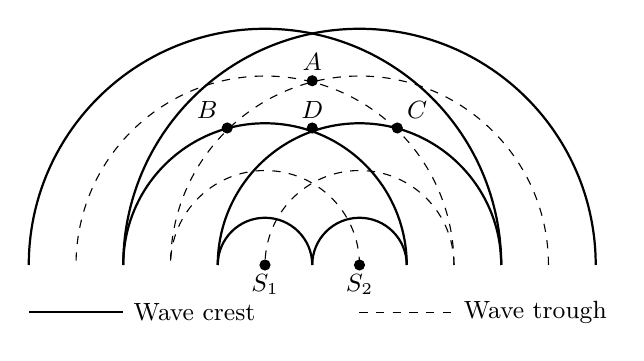
\begin{tikzpicture}[font=\small,scale=1.2]
        \foreach \i in {0.5,1.5,2.5} {
            \draw[thick] (-0.5,0) ++(\i,0) arc(0:180:\i cm);
            \draw[thick] (+0.5,0) ++(\i,0) arc(0:180:\i cm);
        }
        \foreach \j in {1.0,2.0} {
            \draw[dashed] (-0.5,0) ++(\j,0) arc(0:180:\j cm);
            \draw[dashed] (+0.5,0) ++(\j,0) arc(0:180:\j cm);
        }
        %% S_1 and S_2
        \draw[fill] (-0.5,0) circle (1.5pt) node[anchor=north] {$S_1$};
        \draw[fill] (+0.5,0) circle (1.5pt) node[anchor=north] {$S_2$};
        %% A, B, C, D
        \draw[fill] (-0.9,1.45) circle (1.5pt) node[anchor=south east] {$B$};
        \draw[fill] (+0.9,1.45) circle (1.5pt) node[anchor=south west] {$C$};
        \draw[fill] (0,1.95) circle (1.5pt) node[anchor=south] {$A$};
        \draw[fill] (0,1.45) circle (1.5pt) node[anchor=south] {$D$};
        %% Legend
        \draw[thick] (-3,-0.5) -- (-2,-0.5) node[anchor=west] {Wave crest};
        \draw[dashed] (+0.5,-0.5) -- (+1.5,-0.5) node[anchor=west] {Wave trough};
    \end{tikzpicture}
    \end{center}
    At which two points is constructive interference occurring?
    \begin{multicols}{2}
    \begin{choices}
        \wrongchoice{$A$ and $B$}
      \correctchoice{$A$ and $D$}
        \wrongchoice{$B$ and $C$}
        \wrongchoice{$B$ and $D$}
    \end{choices}
    \end{multicols}
\end{question}
}


%% Section June2011
%%--------------------
\element{nysed}{
\begin{question}{June2011-Q16}
    The diagram below represents a view from above of a tank of water in which parallel wave fronts are traveling toward a barrier.
    \begin{center}
    \begin{tikzpicture}
        %% water tank
        \node[anchor=south] at (0,5) {Water Tank};
        \draw[dashed,white!60!black] (-4,0) rectangle (4,5);
        %% wave fronts
        \foreach \x in {-35,-25,-15} \draw (\x mm,0.5) -- (\x mm,4.5);
        \draw[very thick,->] (-4,2) -- (-1,2) node[pos=0.66,anchor=south] {$v$};
        \node[anchor=south] at (-2.5,0) {Wave fronts};
        %% barrier
        \node[anchor=south west,draw,minimum width=1em,minimum height=5.5cm,pattern=vertical lines,rotate=30] (A) at (3.6,0) {};
        \path (A.north east) ++(300:2) node[anchor=south,rotate=-60] {Barrier};
        %% options
        \foreach \x/\y in {180/A,210/B,240/C,270/D} \draw[very thick,->] (3.6,0) ++ (120:{2/sin(60)}) -- ++(\x:2) node[pos=0.75,anchor=center,shift={({\x-90}:1em)}] {$\y$};
    \end{tikzpicture}
    \end{center}
    Which arrow represents the direction of travel for the wave fronts after being reflected from the barrier?
    \begin{multicols}{4}
    \begin{choices}[o]
        \wrongchoice{$A$}
        \wrongchoice{$B$}
      \correctchoice{$C$}
        \wrongchoice{$D$}
    \end{choices}
    \end{multicols}
\end{question}
}

\element{nysed}{
\begin{question}{June2011-Q25}
    A pulse traveled the length of a stretched spring.
    The pulse transferred:
    \begin{choices}
      \correctchoice{energy, only}
        \wrongchoice{mass, only}
        \wrongchoice{both energy and mass}
        \wrongchoice{neither energy nor mass}
    \end{choices}
\end{question}
}

\element{nysed}{
\begin{question}{June2011-Q26}
    The graph below represents the displacement of a particle in
        a medium over a period of time.
    \begin{center}
    \begin{tikzpicture}
        \begin{axis}[
            clip=false,
            axis y line=left,
            axis x line=center,
            axis line style={->},
            xlabel={time},
            x label style={
                at={(current axis.right of origin)},
                anchor=west,
            },
            x unit=\si{\second},
            xtick={1,2,3,4,5,6},
            ylabel={displacement},
            y unit=\si{\centi\meter},
            ytick={-4,-2,0,2,4},
            xmin=0,xmax=6.4,
            ymin=-5,ymax=5,
            width=0.80\columnwidth,
            height=0.45\columnwidth,
            very thin,
        ]
        \addplot[very thick,smooth,domain=0:2*pi]{4*sin(deg(1.56*x))};
        \end{axis}
    \end{tikzpicture}
    \end{center}
    The amplitude of the wave is:
    \begin{multicols}{2}
    \begin{choices}
        \wrongchoice{\SI{4.0}{\second}}
        \wrongchoice{\SI{6.0}{\second}}
        \wrongchoice{\SI{8}{\centi\meter}}
      \correctchoice{\SI{4}{\centi\meter}}
    \end{choices}
    \end{multicols}
\end{question}
}

\element{nysed}{
\begin{question}{June2011-Q27}
    What is the period of a water wave if \num{4.0} complete waves
        pass a fixed point in \SI{10}{\second}?
    \begin{multicols}{2}
    \begin{choices}
        \wrongchoice{\SI{0.25}{\second}}
        \wrongchoice{\SI{0.40}{\second}}
      \correctchoice{\SI{2.5}{\second}}
        \wrongchoice{\SI{4.0}{\second}}
    \end{choices}
    \end{multicols}
\end{question}
}

\element{nysed}{
\begin{question}{June2011-Q28}
    The diagram below represents a periodic wave.
    \begin{center}
    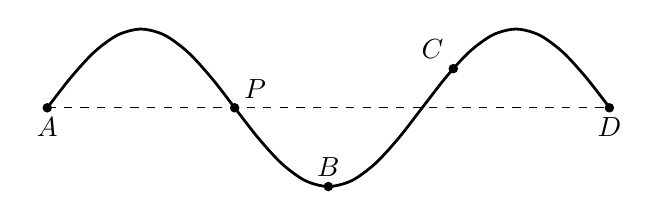
\begin{tikzpicture}[x=0.0625\textwidth]
        %% Graph
        \draw[domain=0:3*pi,smooth,line width=1pt] plot (\x, {sin(\x r)});
        \draw[dashed] (0,0) -- (9.42,0);
        %% Labels
        \node[anchor=north] at (0,0) {$A$};
            \draw[fill] (0,0) circle [radius=1.5pt];
        \node[anchor=south west] at (3.14,0) {$P$};
            \draw[fill] (3.14,0) circle [radius=1.5pt];
        \node[anchor=south] at (4.71,-1) {$B$};
            \draw[fill] (4.71,-1) circle [radius=1.5pt];
        \node[anchor=south east] at (6.804,0.497) {$C$};
            \draw[fill] (6.804,0.497) circle [radius=1.5pt];

        \node[anchor=north] at (9.42,0) {$D$};
            \draw[fill] (9.42,0) circle [radius=1.5pt];
    \end{tikzpicture}
    \end{center}
    Which point on the wave is \ang{90} out of phase with point $P$?
    \begin{multicols}{4}
    \begin{choices}[o]
        \wrongchoice{$A$}
      \correctchoice{$B$}
        \wrongchoice{$C$}
        \wrongchoice{$D$}
    \end{choices}
    \end{multicols}
\end{question}
}

\element{nysed}{
\begin{question}{June2011-Q33}
    Astronauts traveling toward Earth in a fast moving spacecraft
        receive a radio signal from an antenna on Earth.
    Compared to the frequency and wavelength of the radio signal
        from the antenna, the radio signal received by the astronauts has a:
    \begin{choices}
        \wrongchoice{lower frequency and a shorter wavelength}
        \wrongchoice{lower frequency and a longer wavelength}
      \correctchoice{higher frequency and a shorter wavelength}
        \wrongchoice{higher frequency and a longer wavelength}
    \end{choices}
\end{question}
}

\element{nysed}{
\begin{question}{June2011-Q46}
    The diagram below represents a transverse water wave propagating toward the left.
    A cork is floating on the water's surface at point $P$.
    \begin{center}
    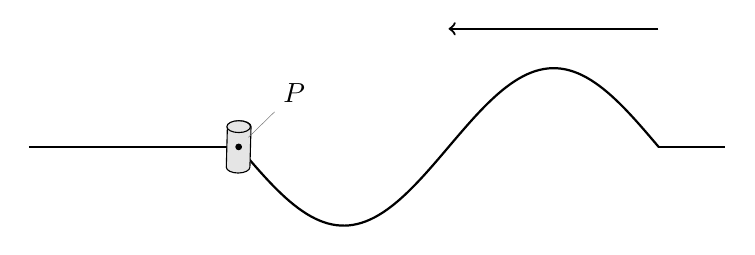
\begin{tikzpicture}[x=0.07\textwidth]
        %% Wave
        \draw[thick] (-3.14,0) -- (0,0);
        \draw[thick,domain=0:2*pi,samples=100] plot (\x, {-1*sin(\x r)});
        \draw[thick] (6.28,0) -- (7.28,0);
        %% Cork
        \node[fill=white!90!black,minimum height=0.5cm,minimum width=0.3cm] (C) at (0,0) {};
        %% make cork 3d
        \draw[fill=white!90!black] (C.south west) arc(180:360:0.15cm and 0.075cm) -- (C.north east) arc(0:180:0.15cm and 0.075cm) -- (C.south west);
        \draw[fill=white!90!black] (C.north) circle (0.15cm and 0.075cm);
        \draw[fill] (0,0) circle (1pt) node[pin=45:$P$] {};
        %% Arrow
        \draw[thick,->] (6.28,1.5) -- (3.14,1.5);
    \end{tikzpicture}
    \end{center}
    In which direction will the cork move as the wave passes point $P$?
    \begin{choices}
        \wrongchoice{up, then down, then up}
      \correctchoice{down, then up, then down}
        \wrongchoice{left, then right, then left}
        \wrongchoice{right, then left, then right}
    \end{choices}
\end{question}
}

\element{nysed}{
\begin{question}{June2011-Q47}
    The diagram below shows a series of wave fronts
        approaching an opening in a barrier.
    Point $P$ is located on the opposite side of the barrier
    \begin{center}
    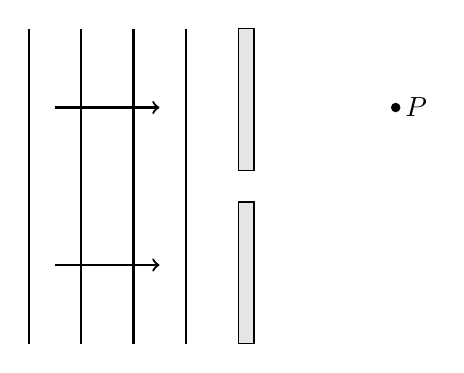
\begin{tikzpicture}
        %% Incoming
        \foreach \i in {0.66,1.33,2.00,2.66} {
            \draw[thick] (-\i,0) -- (-\i,4);
        }
        \draw[thick,->] (-2.33,3) -- (-1.00,3);
        \draw[thick,->] (-2.33,1) -- (-1.00,1);
        %% Barrier
        \draw[fill=white!90!black] (0,0) rectangle (0.2,1.8);
        \draw[fill=white!90!black] (0,2.2) rectangle (0.2,4);
        %% Point P
        \draw[fill] (2,3) circle (1.5pt) node[anchor=west] {$P$};
    \end{tikzpicture}
    \end{center}
    The wave fronts reach point $P$ as a result of:
    \begin{multicols}{2}
    \begin{choices}
        \wrongchoice{resonance}
        \wrongchoice{refraction}
        \wrongchoice{reflection}
      \correctchoice{diffraction}
    \end{choices}
    \end{multicols}
\end{question}
}

\element{nysed}{
\begin{question}{June2011-Q48}
    The diagram below represents a standing wave.
    \begin{center}
    \begin{tikzpicture}[x=0.05\textwidth,yscale=1.0]
        %% Waves
        \draw[domain=0:5*pi,smooth,very thick] plot (\x, {sin(\x r)});
        \draw[domain=0:5*pi,smooth,very thick,dashed] plot (\x, {-1*sin(\x r)});
        %% Walls
        \draw[thick] (0,1) -- (0,-1);
        \draw[thick] (15.7,1) -- (15.7,-1);
        \node[anchor=east,fill,pattern=north east lines,minimum width=0.1cm, minimum height=2cm] at (0,0) {};
        \node[anchor=west,fill,pattern=north east lines,minimum width=0.1cm, minimum height=2cm] at (15.7,0) {};
    \end{tikzpicture}
    \end{center}
    The number of nodes and antinodes shown in the diagram is:
    \begin{choices}
        \wrongchoice{\num{4} nodes and \num{5} antinodes}
        \wrongchoice{\num{5} nodes and \num{6} antinodes}
      \correctchoice{\num{6} nodes and \num{5} antinodes}
        \wrongchoice{\num{6} nodes and \num{10} antinodes}
    \end{choices}
\end{question}
}

\element{nysed}{
\begin{question}{June2011-Q50}
    The diagram below shows two waves traveling in the same medium.
    Points $A$, $B$, $C$, and $D$ are located along the rest position of the medium.
    The waves interfere to produce a resultant wave.
    \begin{center}
    \begin{tikzpicture}
        \begin{axis}[
            clip=false,
            axis y line=left,
            axis x line=center,
            axis line style={->},
            xtick=\empty,
            ylabel={displacement},
            y unit=\si{\meter},
            ytick={-0.3,-0.2,-0.1,0,0.1,0.2,0.3},
            xmin=0,xmax=6.5,
            ymin=-0.35,ymax=0.35,
            width=0.95\columnwidth,
            height=0.618\columnwidth,
            very thin,
        ]
        %% Waves
        \addplot[thick,smooth,domain=0:2*pi]{0.3*sin(deg(x))};
        \addplot[thick,smooth,domain=0:2*pi]{0.1*sin(deg(2*x))};
        %% Labels
        \node[at={(axis cs:0.785,0)},below] {$A$};
        \node[at={(axis cs:2.355,0)},above] {$B$};
        \node[at={(axis cs:3.925,0)},below] {$C$};
        \node[at={(axis cs:5.495,0)},above] {$D$};
        %% Circles
        \draw[fill] (axis cs:0.785,0) circle [radius=1.5pt];
        \draw[fill] (axis cs:2.355,0) circle [radius=1.5pt];
        \draw[fill] (axis cs:3.925,0) circle [radius=1.5pt];
        \draw[fill] (axis cs:5.495,0) circle [radius=1.5pt];
        \end{axis}
    \end{tikzpicture}
    \end{center}
    The superposition of the waves produces the greatest positive
        displacement of the medium from its rest position at point:
    \begin{multicols}{4}
    \begin{choices}[o]
      \correctchoice{$A$}
        \wrongchoice{$B$}
        \wrongchoice{$C$}
        \wrongchoice{$D$}
    \end{choices}
    \end{multicols}
\end{question}
}


%% Section June2010
%%--------------------
\newcommand{\nysedJuneOneZeroQtwentyFour}{
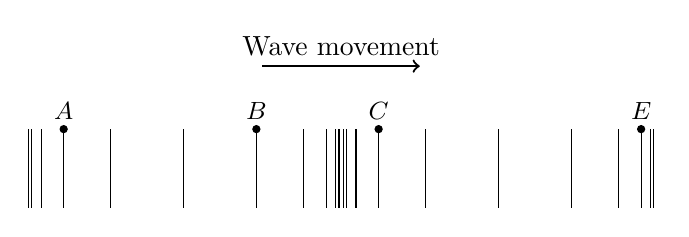
\begin{tikzpicture}
    %% wave fronts
    \foreach \x in {0,1}
        \foreach \y in {-5,-4,...,5} {
            \draw ({4*\x + (4/(1 + exp(-\y)))},0) -- ({4*\x + (4/(1 + exp(-\y)))},1);
        }
    %% wave movement
    \draw[thick,->] (3,1.8) -- (5,1.8) node[pos=0.5,anchor=south] {Wave movement};
    %% options
    \foreach \x/\y/\z in {0/-2/A,0/1/B,1/-2/C,1/3/E}
        \fill ({4*\x + (4/(1 + exp(-\y)))},1) circle (1.5pt) node[anchor=south,font=\small] {$\z$};
\end{tikzpicture}
}

\element{nysed}{
\begin{question}{June2010-Q24}
    A longitudinal wave moves to the right through a uniform medium,
        as shown below.
    Points $A$, $B$, $C$, $D$, and $E$ represent the positions of particles of the medium.
    \begin{center}
        \nysedJuneOneZeroQtwentyFour
    \end{center}
    Which diagram best represents the motion of the particles at position $C$ as the wave moves to the right?
    \begin{multicols}{2}
    \begin{choices}
        \AMCboxDimensions{down=-0.8cm}
        \correctchoice{
            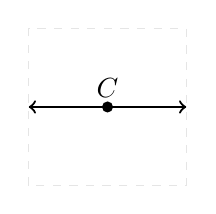
\begin{tikzpicture}[scale=2]
                \draw[dashed,white!90!black] (0,0) rectangle (1,1);
                \fill (0.5,0.5) circle (1pt) node[anchor=south] {$C$};
                \draw[thick,<->] (0,0.5) -- (1,0.5);
            \end{tikzpicture}
        }
        \wrongchoice{
            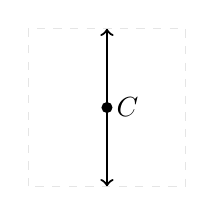
\begin{tikzpicture}[scale=2]
                \draw[dashed,white!90!black] (0,0) rectangle (1,1);
                \fill (0.5,0.5) circle (1pt) node[anchor=west] {$C$};
                \draw[thick,<->] (0.5,0) -- (0.5,1);
            \end{tikzpicture}
        }
        \wrongchoice{
            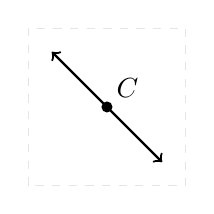
\begin{tikzpicture}[scale=2]
                \draw[dashed,white!90!black] (0,0) rectangle (1,1);
                \fill (0.5,0.5) circle (1pt) node[anchor=south west] {$C$};
                \draw[thick,<->] (0.15,0.85) -- (0.85,0.15);
            \end{tikzpicture}
        }
        \wrongchoice{
            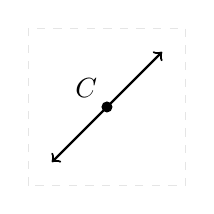
\begin{tikzpicture}[scale=2]
                \draw[dashed,white!90!black] (0,0) rectangle (1,1);
                \fill (0.5,0.5) circle (1pt) node[anchor=south east] {$C$};
                \draw[thick,<->] (0.15,0.15) -- (0.85,0.85);
            \end{tikzpicture}
        }
    \end{choices}
    \end{multicols}
\end{question}
}

\element{nysed}{
\begin{question}{June2010-Q25}
    A longitudinal wave moves to the right through a uniform medium,
        as shown below.
    Points $A$, $B$, $C$, $D$, and $E$ represent the positions of particles of the medium.
    \begin{center}
        \nysedJuneOneZeroQtwentyFour
    \end{center}
    The wavelength of this wave is equal to the distance between points:
    \begin{multicols}{2}
    \begin{choices}
        \wrongchoice{$A$ and $B$}
      \correctchoice{$A$ and $C$}
        \wrongchoice{$B$ and $C$}
        \wrongchoice{$B$ and $E$}
    \end{choices}
    \end{multicols}
\end{question}
}

\element{nysed}{
\begin{question}{June2010-Q26}
    A longitudinal wave moves to the right through a uniform medium,
        as shown below.
    Points $A$, $B$, $C$, $D$, and $E$ represent the positions of particles of the medium.
    \begin{center}
        \nysedJuneOneZeroQtwentyFour
    \end{center}
    The energy of this wave is related to its:
    \begin{multicols}{2}
    \begin{choices}
      \correctchoice{amplitude}
        \wrongchoice{period}
        \wrongchoice{speed}
        \wrongchoice{wavelength}
    \end{choices}
    \end{multicols}
\end{question}
}

\element{nysed}{
\begin{question}{June2010-Q35}
    As viewed from Earth,
        the light from a star has lower frequencies than the lithe emitted by the start because the star is:
    \begin{choices}
        \wrongchoice{moving toward Earth}
      \correctchoice{moving away from Earth}
        \wrongchoice{stationary}
    \end{choices}
\end{question}
}

\element{nysed}{
\begin{question}{June2010-Q48}
    The diagram below represents a periodic wave traveling through a uniform medium.
    \begin{center}
    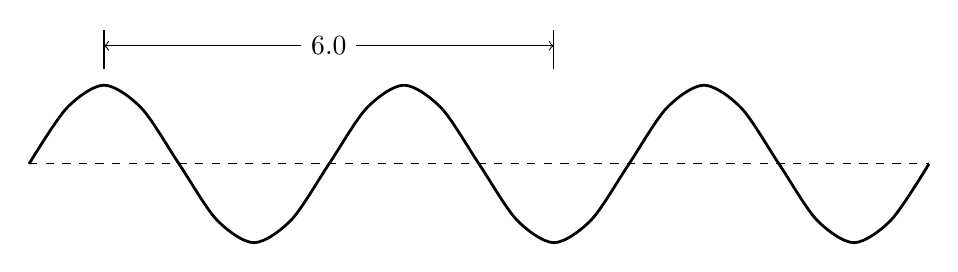
\begin{tikzpicture}[x=0.05\textwidth]
        %% Graph
        \draw[domain=0:6*pi,smooth,line width=1pt] plot (\x, {sin(\x r)});
        \draw[dashed] (0,0) -- (18.84,0);
        %% Labels
        \node[anchor=center] (A) at (6.28,1.5) {\SI{6.0}{\meter}};
        \draw (1.57,1.2) -- (1.57,1.7);
        \draw (10.99,1.2) -- (10.99,1.7);
        \draw[->] (A) -- (1.57,1.5);
        \draw[->] (A) -- (10.99,1.5);
    \end{tikzpicture}
    \end{center}
    If the frequency of the wave is \SI{2.0}{\hertz},
        the speed of the wave is:
    \begin{multicols}{2}
    \begin{choices}
        \wrongchoice{\SI{6.0}{\meter\per\second}}
        \wrongchoice{\SI{2.0}{\meter\per\second}}
      \correctchoice{\SI{8.0}{\meter\per\second}}
        \wrongchoice{\SI{4.0}{\meter\per\second}}
    \end{choices}
    \end{multicols}
\end{question}
}

\element{nysed}{
\begin{question}{June2010-Q50}
    The diagram below shows a standing wave in a string clamped at each end.
    \begin{center}
    \begin{tikzpicture}[x=0.07\textwidth]
        %% Waves
        \draw[domain=0:4*pi,smooth,very thick] plot (\x, {sin(\x r)});
        \draw[domain=0:4*pi,smooth,very thick,dashed] plot (\x, {-1*sin(\x r)});
        %% Walls
        \draw[thick] (0,1) -- (0,-1);
        \draw[thick] (12.56,1) -- (12.56,-1);
        \node[anchor=east,fill,pattern=north east lines,minimum width=0.1cm, minimum height=2cm] at (0,0) {};
        \node[anchor=west,fill,pattern=north east lines,minimum width=0.1cm, minimum height=2cm] at (12.56,0) {};
    \end{tikzpicture}
    \end{center}
    What is the total number of nodes and antinodes in the standing wave?
    \begin{choices}
        \wrongchoice{3 nodes and 2 antinodes}
        \wrongchoice{2 nodes and 3 antinodes}
      \correctchoice{5 nodes and 4 antinodes}
        \wrongchoice{4 nodes and 5 antinodes}
    \end{choices}
\end{question}
}


%% Section June2009
%%--------------------
\element{nysed}{
\begin{question}{June2009-Q24}
    Which type of wave requires a material medium through which to travel?
    \begin{multicols}{2}
    \begin{choices}
      \correctchoice{sound}
        \wrongchoice{radio}
        \wrongchoice{television}
        \wrongchoice{x-ray}
    \end{choices}
    \end{multicols}
\end{question}
}

\element{nysed}{
\begin{question}{June2009-Q25}
    A periodic wave is produced by a vibrating tuning fork.
    The amplitude of the wave would be greater if the tuning fork were:
    \begin{choices}
        \wrongchoice{struck more softly}
      \correctchoice{struck harder}
        \wrongchoice{replaced by a lower frequency tuning fork}
        \wrongchoice{replaced by a higher frequency tuning fork}
    \end{choices}
\end{question}
}

\element{nysed}{
\begin{question}{June2009-Q29}
    The diagram below shows two pulses approaching each other in a uniform medium.
    \begin{center}
    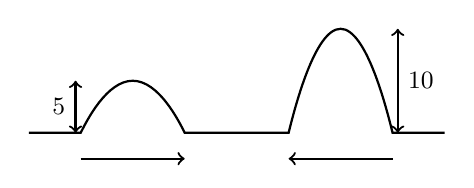
\begin{tikzpicture}[font=\small,scale=0.66]
        \draw[thick] (-4,0) -- (-3,0) parabola bend (-2,1) (-1,0)
                            -- (1,0) parabola bend (2,2) (3,0) -- (4,0);
        %% Arrows
        \draw[thick,->] (-3,-0.5) -- (-1,-0.5);
        \draw[thick,->] (3,-0.5) -- (1,-0.5);
        %% Size Labels
        \draw[thick,<->] (-3.1,0) -- (-3.1,1)
            node[pos=0.5,anchor=east] {\SI{5}{\centi\meter}};
        \draw[thick,<->] (3.1,0) -- (3.1,2)
            node[pos=0.5,anchor=west] {\SI{10}{\centi\meter}};
    \end{tikzpicture}
    \end{center}
    Which diagram best represents the superposition of the two pulses?
    \begin{multicols}{2}
    \begin{choices}
        \AMCboxDimensions{down=-0.5cm}
        \correctchoice{
            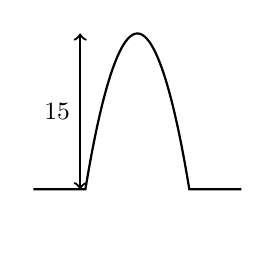
\begin{tikzpicture}[font=\small,scale=0.66]
                \draw[white] (-0.1,-1.1) rectangle (4.1,3.1);
                \draw[thick] (0,0) -- (1,0) parabola bend (2,3) (3,0) -- (4,0);
                \draw[thick,<->] (0.9,0) -- (0.9,3)
                    node[pos=0.5,anchor=east] {\SI{15}{\centi\meter}};
            \end{tikzpicture}
        }
        \wrongchoice{
            \begin{tikzpicture}[font=\small,scale=0.66]
                \draw[white] (-0.1,-1.1) rectangle (4.1,3.1);
                \draw[thick] (0,0) -- (1,0) parabola bend (2,1) (3,0) -- (4,0);
                \draw[thick,<->] (0.9,0) -- (0.9,1)
                    node[pos=0.5,anchor=east] {\SI{5}{\centi\meter}};
            \end{tikzpicture}
        }
        \wrongchoice{
            \begin{tikzpicture}[font=\small,scale=0.66]
                \draw[white] (-0.1,-1.1) rectangle (4.1,3.1);
                \draw[thick] (0,0) -- (1,0) parabola bend (2,1.5) (3,0) -- (4,0);
                \draw[thick,<->] (0.9,0) -- (0.9,1.5)
                    node[pos=0.5,anchor=east] {\SI{7.5}{\centi\meter}};
            \end{tikzpicture}
        }
        \wrongchoice{
            \begin{tikzpicture}[font=\small,scale=0.66]
                \draw[white] (-0.1,-1.1) rectangle (4.1,3.1);
                \draw[thick] (0,0) -- (1,0) parabola bend (2,-1) (3,0) -- (4,0);
                \draw[thick,<->] (0.9,0) -- (0.9,-1)
                    node[pos=0.5,anchor=east] {\SI{5}{\centi\meter}};
            \end{tikzpicture}
        }
    \end{choices}
    \end{multicols}
\end{question}
}


%% Section Jan2009
%%--------------------
\element{nysed}{
\begin{question}{Jan2009-Q23}
    Which type of wave requires a material medium through which to travel?
    \begin{choices}
        \wrongchoice{radio waves}
        \wrongchoice{microwaves}
        \wrongchoice{light waves}
      \correctchoice{mechanical waves}
    \end{choices}
\end{question}
}

\element{nysed}{
\begin{question}{Jan2009-Q25}
    If the amplitude of a wave is increased,
        the frequency of the wave will:
    \begin{choices}
        \wrongchoice{decrease}
        \wrongchoice{increase}
      \correctchoice{stay the same}
    \end{choices}
\end{question}
}

\element{nysed}{
\begin{question}{Jan2009-Q26}
    Which unit is equivalent to a meter per second (\si{\meter\per\second})?
    \begin{choices}
        \wrongchoice{hertz second (\si{\hertz\second})}
      \correctchoice{meter hertz (\si{\meter\hertz})}
        \wrongchoice{second per hertz (\si{\second\per\hertz})}
        \wrongchoice{meter per hertz (\si{\meter\per\hertz})}
    \end{choices}
\end{question}
}

\element{nysed}{
\begin{question}{Jan2009-Q29}
    While playing, two children create a standing wave in a rope,
        as shown in the diagram below.
    A third child participates by jumping rope.
    \begin{center}
        %% NOTE: graphic is necessary
        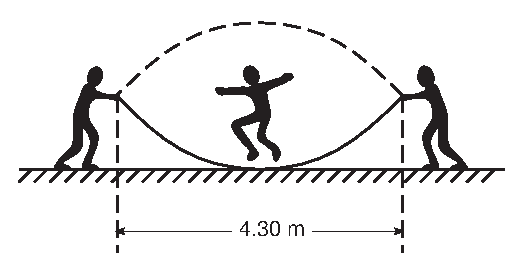
\includegraphics[keepaspectratio,scale=0.75]{Jan2009-Q29}
    \end{center}
    What is the wavelength of this standing wave?
    \begin{multicols}{2}
    \begin{choices}
        \wrongchoice{\SI{2.15}{\meter}}
        \wrongchoice{\SI{4.30}{\meter}}
        \wrongchoice{\SI{6.45}{\meter}}
      \correctchoice{\SI{8.60}{\meter}}
    \end{choices}
    \end{multicols}
\end{question}
}


%% Section June2008
%%--------------------
\element{nysed}{
\begin{question}{June2008-Q25}
    The time required for a wave to complete one full cycle is called the wave's:
    \begin{multicols}{2}
    \begin{choices}
        \wrongchoice{frequency}
        \wrongchoice{velocity}
      \correctchoice{period}
        \wrongchoice{wavelength}
    \end{choices}
    \end{multicols}
\end{question}
}

\element{nysed}{
\begin{question}{June2008-Q27}
    The diagram below represents a transverse wave.
    \begin{center}
    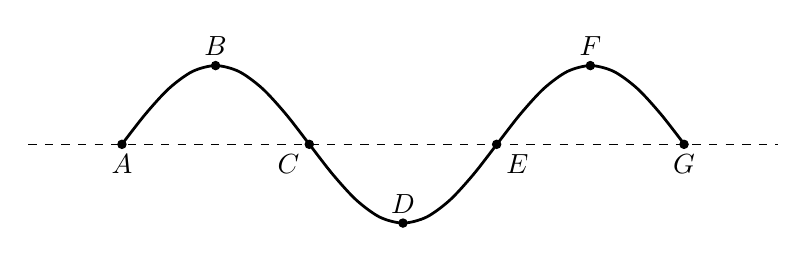
\begin{tikzpicture}[x=0.0625\textwidth]
        %% Graph
        \draw[domain=0:3*pi,smooth,line width=1pt] plot (\x, {sin(\x r)});
        \draw[dashed] (-1.57,0) -- (10.99,0);
        %% Labels
        \node[anchor=north]     at (0,0) {$A$};
        \node[anchor=south]     at (1.57,1) {$B$};
        \node[anchor=north east]at (3.14,0) {$C$};
        \node[anchor=south]     at (4.71,-1) {$D$};
        \node[anchor=north west]at (6.28,0) {$E$};
        \node[anchor=south]     at (7.85,1) {$F$};
        \node[anchor=north]     at (9.42,0) {$G$};
        %% Circles
        \draw[fill] (0,0) circle [radius=1.5pt];
        \draw[fill] (1.57,1) circle [radius=1.5pt];
        \draw[fill] (3.14,0) circle [radius=1.5pt];
        \draw[fill] (4.71,-1) circle [radius=1.5pt];
        \draw[fill] (6.28,0) circle [radius=1.5pt];
        \draw[fill] (7.85,1) circle [radius=1.5pt];
        \draw[fill] (9.42,0) circle [radius=1.5pt];
    \end{tikzpicture}
    \end{center}
    The wavelength of the wave is equal to the distance between points?
    \begin{multicols}{2}
    \begin{choices}
        \wrongchoice{$A$ and $G$}
      \correctchoice{$B$ and $F$}
        \wrongchoice{$C$ and $E$}
        \wrongchoice{$D$ and $F$}
    \end{choices}
    \end{multicols}
\end{question}
}

\element{nysed}{
\begin{question}{June2008-Q30}
    Wave $X$ travels eastward with frequency $f$ and amplitude $A$.
    Wave $Y$, traveling in the same medium,
        interacts with wave $X$ and produces a standing wave.
    Which statement about wave $Y$ is correct?
    \begin{choices}
      \correctchoice{Wave $Y$ must have a frequency of $f$, an amplitude of $A$, and be traveling eastward.}
        \wrongchoice{Wave $Y$ must have a frequency of $2f$, an amplitude of $3A$, and be traveling eastward.}
        \wrongchoice{Wave $Y$ must have a frequency of $3f$, an amplitude of $2A$, and be traveling westward.}
        \wrongchoice{Wave $Y$ must have a frequency of $f$, an amplitude of $A$, and be traveling westward.}
    \end{choices}
\end{question}
}

\element{nysed}{
\begin{question}{June2008-Q31}
    The diagram below represents two pulses approaching each other from opposite directions in the same medium.
    \begin{center}
    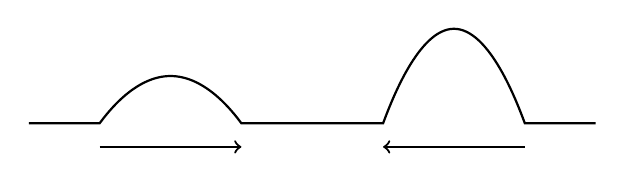
\begin{tikzpicture}[yscale=0.6,xscale=0.9]
        \draw[thick] (-4,0) -- (-3,0) parabola bend (-2,1) (-1,0) -- (1,0) parabola bend (2,2) (3,0) -- (4,0);
        \draw[thick,->] (-3,-0.5) -- (-1,-0.5);
        \draw[thick,->] (3,-0.5) -- (1,-0.5);
    \end{tikzpicture}
    \end{center}
    Which diagram best represents the medium after the pulses have passed through each other?
    \begin{choices}
        \AMCboxDimensions{down=-1.25cm}
        \correctchoice{
            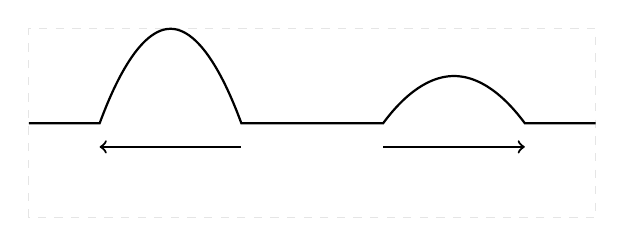
\begin{tikzpicture}[yscale=0.6,xscale=0.9]
                \draw[dashed,white!90!black] (-4,-2) rectangle (4,2);
                \draw[thick] (-4,0) -- (-3,0) parabola bend (-2,2) (-1,0)
                                    -- (1,0) parabola bend (2,1) (3,0) -- (4,0);
                \draw[thick,<-] (-3,-0.5) -- (-1,-0.5);
                \draw[thick,<-] (3,-0.5) -- (1,-0.5);
            \end{tikzpicture}
        }
        \wrongchoice{
            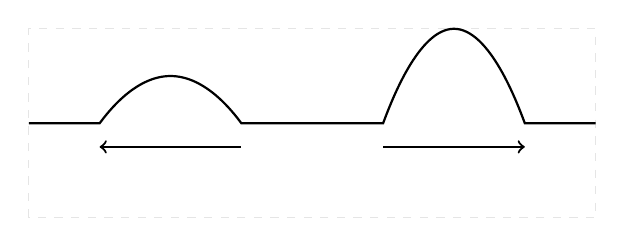
\begin{tikzpicture}[yscale=0.6,xscale=0.9]
                \draw[dashed,white!90!black] (-4,-2) rectangle (4,2);
                \draw[thick] (-4,0) -- (-3,0) parabola bend (-2,1) (-1,0)
                                    -- (1,0) parabola bend (2,2) (3,0) -- (4,0);
                \draw[thick,<-] (-3,-0.5) -- (-1,-0.5);
                \draw[thick,<-] (3,-0.5) -- (1,-0.5);
            \end{tikzpicture}
        }
        \wrongchoice{
            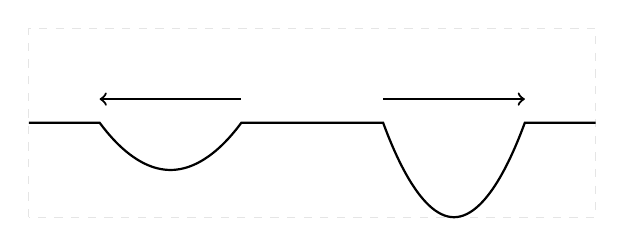
\begin{tikzpicture}[yscale=0.6,xscale=0.9]
                \draw[dashed,white!90!black] (-4,-2) rectangle (4,2);
                \draw[thick] (-4,0) -- (-3,0) parabola bend (-2,-1) (-1,0)
                                    -- (1,0) parabola bend (2,-2) (3,0) -- (4,0);
                \draw[thick,<-] (-3,0.5) -- (-1,0.5);
                \draw[thick,<-] (3,0.5) -- (1,0.5);
            \end{tikzpicture}
        }
        \wrongchoice{
            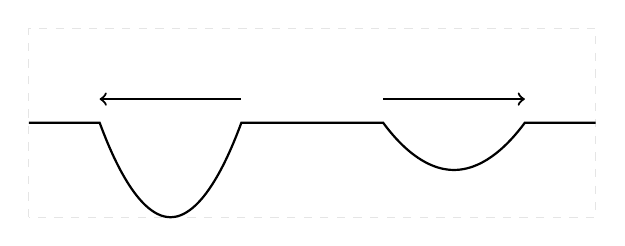
\begin{tikzpicture}[yscale=0.6,xscale=0.9]
                \draw[dashed,white!90!black] (-4,-2) rectangle (4,2);
                \draw[thick] (-4,0) -- (-3,0) parabola bend (-2,-2) (-1,0)
                                    -- (1,0) parabola bend (2,-1) (3,0) -- (4,0);
                \draw[thick,<-] (-3,0.5) -- (-1,0.5);
                \draw[thick,<-] (3,0.5) -- (1,0.5);
            \end{tikzpicture}
        }
    \end{choices}
\end{question}
}

\element{nysed}{
\begin{question}{June2008-Q48}
    The diagram represents a transverse wave traveling to the right through a medium.
    Point $A$ represents a particle of the medium.
    \begin{center}
    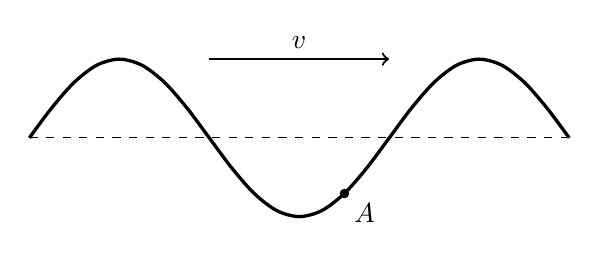
\begin{tikzpicture}[x=0.06\textwidth]
        %% Graph
        \draw[domain=0:3*pi,smooth,very thick] plot (\x, {sin(\x r)});
        \draw[dashed] (0,0) -- (9.42,0);
        %% Vectors
        \draw[thick,->] (3.14,1.0) -- (6.28,1.0)
            node[pos=0.5,anchor=south] {$v$};
        %% Labels
        \draw[fill] (5.50,-0.707) circle [radius=1.5pt]
            node[anchor=north west] {$A$};
    \end{tikzpicture}
    \end{center}
    In which direction will particle $A$ move in the next instance of time?
    \begin{multicols}{2}
    \begin{choices}
        \wrongchoice{up}
      \correctchoice{down}
        \wrongchoice{left}
        \wrongchoice{right}
    \end{choices}
    \end{multicols}
\end{question}
}


%% Section Jan2008
%%--------------------
\element{nysed}{
\begin{question}{Jan2008-Q24}
    The product of a wave's frequency and its period is:
    \begin{multicols}{2}
    \begin{choices}
      \correctchoice{one}
        \wrongchoice{its velocity}
        \wrongchoice{its wavelength}
        \wrongchoice{Planck's constant}
    \end{choices}
    \end{multicols}
\end{question}
}

\element{nysed}{
\begin{question}{Jan2008-Q25}
    A periodic wave having a frequency of \SI{5.0}{\hertz} and a speed of \SI{10}{\meter\per\second} has a wavelength of:
    \begin{multicols}{2}
    \begin{choices}
        \wrongchoice{\SI{0.50}{\meter}}
      \correctchoice{\SI{2.0}{\meter}}
        \wrongchoice{\SI{5.0}{\meter}}
        \wrongchoice{\SI{50}{\meter}}
    \end{choices}
    \end{multicols}
\end{question}
}

\element{nysed}{
\begin{question}{Jan2008-Q31}
    Two pulses traveling in the same uniform medium approach each other,
        as shown in the diagram below.
    \begin{center}
    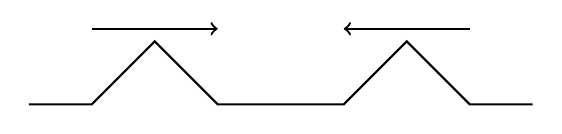
\begin{tikzpicture}[scale=0.8]
        \draw[thick] (0,0) -- (1,0) -- (2,1) -- (3,0) -- (5,0) -- (6,1) -- (7,0) -- (8,0);
        \draw[thick,->] (1,1.2) -- (3,1.2);
        \draw[thick,->] (7,1.2) -- (5,1.2);
    \end{tikzpicture}
    \end{center}
    Which diagram best represents the superposition of the two pulses?
    \begin{multicols}{2}
    \begin{choices}
        \correctchoice{
            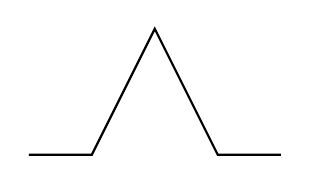
\begin{tikzpicture}[scale=0.8]
                \draw[white] (0,0) rectangle (4,2);
                \draw[thick] (0,0) -- (1,0) -- (2,2) -- (3,0) -- (4,0);
            \end{tikzpicture}
        }
        \wrongchoice{
            \begin{tikzpicture}[scale=0.8]
                \draw[white] (0,0) rectangle (4,2);
                \draw[thick] (0,0) -- (1,0) -- (1,1) -- (3,1) -- (3,0) -- (4,0);
            \end{tikzpicture}
        }
        \wrongchoice{
            \begin{tikzpicture}[scale=0.8]
                \draw[white] (0,0) rectangle (4,2);
                \draw[thick] (0,0) -- (1,0) -- (2,1) -- (3,0) -- (4,0);
            \end{tikzpicture}
        }
        \wrongchoice{
            \begin{tikzpicture}[scale=0.8]
                \draw[white] (0,0) rectangle (4,2);
                \draw[thick] (0,0) -- (4,0);
            \end{tikzpicture}
        }
    \end{choices}
    \end{multicols}
\end{question}
}

\element{nysed}{
\begin{question}{Jan2008-Q34}
    Which diagram best represents the shape and direction of a series of wave fronts after they have passed through a small opening in a barrier?
    \begin{multicols}{2}
    \begin{choices}
        \AMCboxDimensions{down=-0.8cm}
        \wrongchoice{
            \begin{tikzpicture}
                \draw[dashed,white!60!black] (-1.5,-1.2) rectangle (1.5,1.2);
                %% incoming
                \foreach \x in {4,8,12} \draw (-\x mm,-1.2) -- (-\x mm,1.2);
                \foreach \y in {-0.75,0.75} \draw[thick,->] (-1.5,\y) -- (-0.2,\y);
                %% barrier
                \draw[pattern=north east lines] (-0.5ex,-1.2) rectangle (0.5ex,-0.2);
                \draw[pattern=north east lines] (-0.5ex,+1.2) rectangle (0.5ex,+0.2);
                %% outgoing
                \draw[thick,->] (0.5ex,+0.75) -- (1.4,+0.2);
                \draw[thick,->] (0.5ex,-0.75) -- (1.4,-0.2);
                \draw[thick,->] (0.5ex,0) -- (1.2,0);
            \end{tikzpicture}
        }
        \wrongchoice{
            \begin{tikzpicture}
                \draw[dashed,white!60!black] (-1.5,-1.2) rectangle (1.5,1.2);
                %% incoming
                \foreach \x in {4,8,12} \draw (-\x mm,-1.2) -- (-\x mm,1.2);
                \foreach \y in {-0.75,0.75} \draw[thick,->] (-1.5,\y) -- (-0.2,\y);
                %% barrier
                \draw[pattern=north east lines] (-0.5ex,-1.2) rectangle (0.5ex,-0.2);
                \draw[pattern=north east lines] (-0.5ex,+1.2) rectangle (0.5ex,+0.2);
                %% outgoing
                \foreach \x in {4,8,12} \draw (1.5,0) ++(140:\x mm) arc(140:220:\x mm);
                \draw[thick,<-] (1.5,0) ++(150:1ex) -- ++(150:1.3);
                \draw[thick,<-] (1.5,0) ++(210:1ex) -- ++(210:1.3);
            \end{tikzpicture}
        }
        \wrongchoice{
            \begin{tikzpicture}
                \draw[dashed,white!60!black] (-1.5,-1.2) rectangle (1.5,1.2);
                %% incoming
                \foreach \x in {4,8,12} \draw (-\x mm,-1.2) -- (-\x mm,1.2);
                \foreach \y in {-0.75,0.75} \draw[thick,->] (-1.5,\y) -- (-0.2,\y);
                %% barrier
                \draw[pattern=north east lines] (-0.5ex,-1.2) rectangle (0.5ex,-0.2);
                \draw[pattern=north east lines] (-0.5ex,+1.2) rectangle (0.5ex,+0.2);
                %% outgoing
                \foreach \x in {4,8,12} {
                    \draw (0.5ex,0) ++(5:\x mm) arc(5:70:\x mm);
                    \draw (0.5ex,0) ++(355:\x mm) arc(355:290:\x mm);
                }
                \draw[thick,<-] (0.5ex,0) ++ (37:1ex) -- ++(37:1.3);
                \draw[thick,<-] (0.5ex,0) ++ (323:1ex) -- ++(323:1.3);
            \end{tikzpicture}
        }
        %% ANS is D
        \correctchoice{
            \begin{tikzpicture}
                \draw[dashed,white!60!black] (-1.5,-1.2) rectangle (1.5,1.2);
                %% incoming
                \foreach \x in {4,8,12} \draw (-\x mm,-1.2) -- (-\x mm,1.2);
                \foreach \y in {-0.75,0.75} \draw[thick,->] (-1.5,\y) -- (-0.2,\y);
                %% barrier
                \draw[pattern=north east lines] (-0.5ex,-1.2) rectangle (0.5ex,-0.2);
                \draw[pattern=north east lines] (-0.5ex,+1.2) rectangle (0.5ex,+0.2);
                %% outgoing
                \foreach \x in {4,8,12} \draw (0.5ex,0) ++(0,\x mm) arc(90:-90:\x mm);
                \foreach \y in {30,330} \draw[thick,->] (0.5ex,0) ++(\y:0.5ex) -- ++(\y:1.3);
            \end{tikzpicture}
        }
    \end{choices}
    \end{multicols}
\end{question}
}


%% Section June2007
%%--------------------
\element{nysed}{
\begin{question}{June2007-Q22}
    The diagram below represents a transverse wave.
    \begin{center}
    \begin{tikzpicture}[x=0.1\textwidth]
        %% Graph
        \draw[domain=0:2*pi,smooth,very thick] plot (\x, {-1*sin(\x r)});
        \draw[] (0,-1.25) -- (0,1.25);
        \draw[] (0,0) -- (6.28,0);
        %% Labels
        \node[anchor=east]      at (0,0) {$A$};
        \node[anchor=east]      at (0,1) {$D$};
        \node[anchor=east]      at (0,-1) {$E$};
        \node[anchor=north west]at (3.14,0) {$B$};
        \node[anchor=north]     at (6.28,0) {$C$};
        %% Dashed
        \draw[dashed] (0,1) -- (4.71,1);
        \draw[dashed] (0,-1) -- (1.57,-1);
        %% Circles
        \draw[fill] (0,1)   circle [radius=1.5pt];
        \draw[fill] (0,0)   circle [radius=1.5pt];
        \draw[fill] (0,-1)  circle [radius=1.5pt];
        \draw[fill] (3.14,0)circle [radius=1.5pt];
        \draw[fill] (6.28,0)circle [radius=1.5pt];
    \end{tikzpicture}
    \end{center}
    The distance between which two points identifies the amplitude of the wave?
    \begin{multicols}{2}
    \begin{choices}
      \correctchoice{$A$ and $E$}
        \wrongchoice{$A$ and $E$}
        \wrongchoice{$A$ and $C$}
        \wrongchoice{$D$ and $E$}
    \end{choices}
    \end{multicols}
\end{question}
}

\element{nysed}{
\begin{question}{June2007-Q23}
    The diagram below represents a periodic wave.
    \begin{center}
    \begin{tikzpicture}[x=0.0556\textwidth]
        %% Graph
        \draw[domain=0:5*pi,smooth,very thick] plot (\x, {cos(\x r)});
        \draw[] (0,-1.25) -- (0,1.25);
        \draw[] (0,0) -- (16.0,0);
        %% Labels
        \node[anchor=south west]at (0,1) {$A$};
        \node[anchor=north west]at (4.71,0) {$P$};
        \node[anchor=south west]at (7.85,0) {$B$};
        \node[anchor=north west]at (10.99,0) {$C$};
        \node[anchor=south]     at (15.7,-1) {$D$};
        %% Circles
        \draw[fill] (0,1)       circle [radius=1.5pt];
        \draw[fill] (4.71,0)    circle [radius=1.5pt];
        \draw[fill] (7.85,0)    circle [radius=1.5pt];
        \draw[fill] (10.99,0)   circle [radius=1.5pt];
        \draw[fill] (15.7,-1)    circle [radius=1.5pt];
    \end{tikzpicture}
    \end{center}
    Which point on the wave is in phase with point $P$?
    \begin{multicols}{4}
    \begin{choices}[o]
        \wrongchoice{$A$}
        \wrongchoice{$B$}
      \correctchoice{$C$}
        \wrongchoice{$D$}
    \end{choices}
    \end{multicols}
\end{question}
}

\element{nysed}{
\begin{question}{June2007-Q27}
    Which type of wave requires a material medium through which to travel?
    \begin{multicols}{2}
    \begin{choices}
      \correctchoice{sound}
        \wrongchoice{electromagnetic}
        \wrongchoice{infrared}
        \wrongchoice{radio}
    \end{choices}
    \end{multicols}
\end{question}
}

\element{nysed}{
\begin{question}{June2007-Q30}
    Two waves having the same frequency and amplitude are traveling in the same medium.
    Maximum constructive interference occurs at points where the phase difference between the two superposed waves is:
    \begin{multicols}{4}
    \begin{choices}
      \correctchoice{\ang{0}}
        \wrongchoice{\ang{90}}
        \wrongchoice{\ang{180}}
        \wrongchoice{\ang{270}}
    \end{choices}
    \end{multicols}
\end{question}
}


%% Section Jan2007
%%--------------------
\element{nysed}{
\begin{question}{Jan2007-Q21}
    If the amplitude of a wave traveling in a rope is doubled,
        the speed of the wave in the rope will:
    \begin{choices}
      \correctchoice{remain the same}
        \wrongchoice{decrease}
        \wrongchoice{increase}
    \end{choices}
\end{question}
}

\element{nysed}{
\begin{question}{Jan2007-Q22}
    Two waves having the same amplitude and frequency are traveling in the same medium.
    Maximum destructive interference will occur when the phase difference between the waves is:
    \begin{multicols}{4}
    \begin{choices}
      \correctchoice{\ang{180}}
        \wrongchoice{\ang{0}}
        \wrongchoice{\ang{270}}
        \wrongchoice{\ang{90}}
    \end{choices}
    \end{multicols}
\end{question}
}

\element{nysed}{
\begin{question}{Jan2007-Q24}
    A ringing bell is located in a chamber.
    When the air is removed from the chamber,
        why can the bell be seen vibrating but \emph{not} be heart?
    \begin{choices}
      \correctchoice{Light waves can travel through a vacuum, but sound waves cannot.}
        \wrongchoice{Light waves travel slower than sound waves.}
        \wrongchoice{Sound waves have greater amplitude than light waves.}
        \wrongchoice{Sound waves have higher frequency than light waves.}
    \end{choices}
\end{question}
}

\element{nysed}{
\begin{question}{Jan2007-Q25}
    As a transverse wave travels through a medium,
        the individual particles of the medium move:
    \begin{choices}
      \correctchoice{perpendicular to the direction of wave travel}
        \wrongchoice{parallel to the direction of wave travel}
        \wrongchoice{in circles}
        \wrongchoice{in ellipses}
    \end{choices}
\end{question}
}

\element{nysed}{
\begin{question}{Jan2007-Q28}
    Parallel wave fronts incident on an opening in a barrier are diffracted.
    For which combination of wavelength and size of opening will diffraction effects be greatest?
    \begin{choices}
      \correctchoice{long wavelength and narrow opening}
        \wrongchoice{long wavelength and wide opening}
        \wrongchoice{short wavelength and narrow opening}
        \wrongchoice{short wavelength and wide opening}
    \end{choices}
\end{question}
}

\element{nysed}{
\begin{question}{Jan2007-Q49}
    The diagram below represents a wave.
    \begin{center}
    \begin{tikzpicture}[x=0.035\textwidth]
        %% Wave
        \draw[domain=0:6*pi,smooth,very thick] plot (\x, {sin(\x r)});
        %% Y Label
        \draw (0,-1.5) -- (0,1.2);
        \draw (18.84,-1.5) -- (18.84,1.2);
        \node[anchor=east] (X1) at (-0.5,1.0) {\SI{0.20}{\meter}};
        \node[anchor=east] (X2) at (-0.5,-1.0) {\SI{-0.20}{\meter}};
        \draw[dashed] (X1) -- (18.84,1.0);
        \draw[dashed] (X2) -- (18.84,-1.0);
        \draw[dashed] (0,0) -- (18.84,0.0);
        %% X Label
        \node[anchor=center] (X4) at (9.42,-1.3) {\SI{6.00}{\meter}};
        \draw[->] (X4) -- (0,-1.3);
        \draw[->] (X4) -- (18.84,-1.3);
    \end{tikzpicture}
    \end{center}
    What is the speed of the wave if its frequency is \SI{8.0}{\hertz}?
    \begin{multicols}{2}
    \begin{choices}
      \correctchoice{\SI{16}{\meter\per\second}}
        \wrongchoice{\SI{48}{\meter\per\second}}
        \wrongchoice{\SI{1.6}{\meter\per\second}}
        \wrongchoice{\SI{3.2}{\meter\per\second}}
    \end{choices}
    \end{multicols}
\end{question}
}


%% Section June2006
%%--------------------
\element{nysed}{
\begin{question}{June2006-Q28}
    The diagram below represents straight fronts passing from deep water into shallow water,
        with a change in speed and direction.
    \begin{center}
    \begin{tikzpicture}
        %% deep water
        \draw[thick,latex-]  (1,2) -- (1,3.5) node[anchor=north] {Deep water};
        \foreach \y in {1.5,2.0,2.5,3.0} \draw[thick] (0,\y) -- ({1.5*(\y+0.66)},\y) -- ++(20:{2.3-1.85*(\y-3)});
        %% boundary
        \draw[line width=2pt] (1,0) -- (7,4) node[pos=0.2,anchor=north,rotate=34] {Boundary};
        \draw[thick,-latex] (1,0) ++(33.69:5.5) ++(290:1ex) -- ++(290:1) node[anchor=north] {Shallow water};
    \end{tikzpicture}
    \end{center}
    Which phenomenon is illustrated in the diagram?
    \begin{multicols}{2}
    \begin{choices}
      \correctchoice{refraction}
        \wrongchoice{reflection}
        \wrongchoice{diffraction}
        \wrongchoice{interference}
    \end{choices}
    \end{multicols}
\end{question}
}

\element{nysed}{
\begin{question}{June2006-Q32}
    Two waves traveling in the same medium and having the same wavelength ($\lambda$) interfere to create a standing wave.
    What is the distance between two consecutive nodes on this standing wave?
    \begin{multicols}{4}
    \begin{choices}
      \correctchoice{$\dfrac{\lambda}{2}$}
        \wrongchoice{$\lambda$}
        \wrongchoice{$\dfrac{\lambda}{4}$}
        \wrongchoice{$\dfrac{3\lambda}{4}$}
    \end{choices}
    \end{multicols}
\end{question}
}

\element{nysed}{
\begin{question}{June2006-Q33}
    An earthquake wave is traveling from west to east through rock.
    If the particles of the rock are vibrating in a north-south direction,
        the wave must be classified as:
    \begin{multicols}{2}
    \begin{choices}
      \correctchoice{transverse}
        \wrongchoice{longitudinal}
        \wrongchoice{a microwave}
        \wrongchoice{a radio wave}
    \end{choices}
    \end{multicols}
\end{question}
}

\element{nysed}{
\begin{question}{June2006-Q46}
    The diagram represents two pulses approaching each other.
    \begin{center}
    \begin{tikzpicture}[scale=0.8]
        \draw[thick] (0,0) -- (1,0) -- (1,1) -- (2,1) -- (2,0) -- (4,0) -- (4,-2) -- (5,-2) -- (5,0) -- (6,0);
        \draw[thick,->] (1,1.5) -- (2,1.5);
        \draw[thick,->] (5,1.5) -- (4,1.5);
    \end{tikzpicture}
    \end{center}
    Which diagram best represents the resultant pulse at the instant the pulses are passing through each other?
    \begin{multicols}{2}
    \begin{choices}
        \AMCboxDimensions{down=-1.5cm}
        \correctchoice{
            \begin{tikzpicture}[scale=0.8]
                \draw[white] (0,-2) rectangle (3,1);
                \draw[thick] (0,0) -- (1,0) -- (1,-1) -- (2,-1) -- (2,0) -- (3,0);
            \end{tikzpicture}
        }
        \wrongchoice{
            \begin{tikzpicture}[scale=0.8]
                \draw[white] (0,-2) rectangle (3,1);
                \draw[thick] (0,0) -- (1,0) -- (1,-2) -- (2,-2) -- (2,0) -- (3,0);
            \end{tikzpicture}
        }
        \wrongchoice{
            \begin{tikzpicture}[scale=0.8]
                \draw[white] (0,-2) rectangle (3,1);
                \draw[thick] (0,0) -- (1,0) -- (1,1) -- (2,1) -- (2,0) -- (3,0);
            \end{tikzpicture}
        }
        \wrongchoice{
            \begin{tikzpicture}[scale=0.8]
                \draw[white] (0,-2) rectangle (3,1);
                \draw[thick] (0,0) -- (3,0);
            \end{tikzpicture}
        }
    \end{choices}
    \end{multicols}
\end{question}
}


%% Section Jan2006
%%--------------------
\element{nysed}{
\begin{question}{Jan2006-Q28}
    A sonar wave is reflected from the ocean floor.
    For which angles of incidence do the wave's angle of reflection equal its angle of incidence?
    \begin{choices}
        \wrongchoice{angles less than \ang{45}, only}
        \wrongchoice{an angle of \ang{45}, only}
        \wrongchoice{angles greater than \ang{45}, only}
      \correctchoice{all angles of incidence}
    \end{choices}
\end{question}
}

\element{nysed}{
\begin{question}{Jan2006-Q29}
    How are electromagnetic waves that are produced by oscillating charges and sound waves that are produced by oscillating tuning forks similar?
    \begin{choices}
      \correctchoice{Both have the same frequency as their respective sources.}
        \wrongchoice{Both require a matter medium for propagation.}
        \wrongchoice{Both are longitudinal waves.}
        \wrongchoice{Both are transverse waves.}
    \end{choices}
\end{question}
}

\element{nysed}{
\begin{question}{Jan2006-Q30}
    The diagram below represents a transverse wave traveling in a string.
    \begin{center}
    \begin{tikzpicture}[x=0.0625\textwidth]
        %% Graph
        \draw[domain=0:4*pi,smooth,line width=1pt] plot (\x, {sin(\x r)});
        \draw (0,0) -- (13.00,0);
        \draw (0,-1.2) -- (0,1.2);
        %% Labels
        \node[anchor=north west]at (0,0)    {$A$};
            \draw[fill] (0,0) circle [radius=1.5pt];
        \node[anchor=north]     at (1.57,1) {$B$};
            \draw[fill] (1.57,1) circle [radius=1.5pt];
        \node[anchor=south west]at (3.14,0) {$C$};
            \draw[fill] (3.14,0) circle [radius=1.5pt];
        \node[anchor=south]     at (4.71,-1) {$D$};
            \draw[fill] (4.71,-1) circle [radius=1.5pt];
        \node[anchor=north west]at (6.28,0){$E$};
            \draw[fill] (6.28,0) circle [radius=1.5pt];
        \node[anchor=north]     at (7.85,1){$F$};
            \draw[fill] (7.85,1) circle [radius=1.5pt];
        \node[anchor=south west]at (9.42,0){$G$};
            \draw[fill] (9.42,0) circle [radius=1.5pt];
        \node[anchor=south]     at (10.99,-1){$H$};
            \draw[fill] (10.99,-1) circle [radius=1.5pt];
    \end{tikzpicture}
    \end{center}
    Which two labeled points are \ang{180} out of phase?
    \begin{multicols}{2}
    \begin{choices}
      \correctchoice{$D$ and $F$}
        \wrongchoice{$B$ and $F$}
        \wrongchoice{$A$ and $D$}
        \wrongchoice{$D$ and $H$}
    \end{choices}
    \end{multicols}
\end{question}
}

\element{nysed}{
\begin{question}{Jan2006-Q32}
    The diagram below represents shallow water waves of constant wavelength passing through two small opening, $A$ and $B$, in a barrier.
    \begin{center}
    %% NOTE: June1996-Q42
    \begin{tikzpicture}
        %% incoming
        \foreach \x in {5,15}
            \draw[dashed] (-4,-\x mm) -- (4,-\x mm);
        \foreach \x in {10,20}
            \draw[thick] (-4,-\x mm) -- (4,-\x mm);
        %% outcoming A
        \foreach \x in {5,15,25}  {
            \draw[dashed] (-1,0.25ex) ++(\x mm,0) arc (0:180:\x mm);
            \draw[dashed] (+1,0.25ex) ++(\x mm,0) arc (0:180:\x mm);
        }
        \foreach \x in {10,20,30} {
            \draw[thick] (-1,0.25ex) ++(\x mm,0) arc (0:180:\x mm);
            \draw[thick] (+1,0.25ex) ++(\x mm,0) arc (0:180:\x mm);
        }
        %% barrier
        \draw[fill=white!50!black] (-4,-0.25ex) rectangle (-1.1,0.25ex);
        \draw[fill=white!50!black] (-0.9,-0.25ex) rectangle (0.9,0.25ex);
        \draw[fill=white!50!black] (1.1,-0.25ex) rectangle (4.0,0.25ex);
        %% labels
        \node[anchor=north] at (-1,0) {$A$};
        \node[anchor=north] at (+1,0) {$B$};
        \fill (6.8mm,25.3mm) circle (2pt) node[anchor=south west] {$P$};
        %% Legend
        \draw (-2.5,-2.5) -- (-1.5,-2.5) node[anchor=west] {Crests};
        \draw[dashed] (0.5,-2.5) -- (1.5,-2.5) node[anchor=west] {Troughs};
    \end{tikzpicture}
    \end{center}
    Which statement best describes the interference at point $P$?
    \begin{choices}
      \correctchoice{It is destructive, and causes a decrease in amplitude.}
        \wrongchoice{It is destructive, and causes a shorter wavelength.}
        \wrongchoice{It is constructive, and causes an increase in amplitude.}
        \wrongchoice{It is constructive, and causes a longer wavelength.}
    \end{choices}
\end{question}
}


%% Section June2005
%%--------------------
\element{nysed}{
\begin{question}{June2005-Q24}
    A transverse wave passes through a uniform material medium from left to right,
        as shown in the diagram below.
    \begin{center}
    \begin{tikzpicture}[x=0.0625\textwidth]
        %% Wave
        \draw[domain=0:3.5*pi,smooth,line width=1pt] plot (\x, {sin(\x r)});
        %% Vector
        \draw[->] (4.0,1.5) -- (7.0,1.5)
            node[pos=0.5,anchor=south] {$v$};
    \end{tikzpicture}
    \end{center}
    Which diagram best represents the direction of vibration of the particles of the medium?
    \begin{multicols}{2}
    \begin{choices}
        \AMCboxDimensions{down=-0.8cm}
        \correctchoice{
            \begin{tikzpicture}
                \draw[dashed,white!90!black] (-1,-1) rectangle (1,1);
                \draw[fill] (0,0) circle (1pt);
                \draw[thick,<->] (270:1) -- (90:1);
            \end{tikzpicture}
        }
        \wrongchoice{
            \begin{tikzpicture}
                \draw[dashed,white!90!black] (-1,-1) rectangle (1,1);
                \draw[fill] (0,0) circle (1pt);
                \draw[thick,<->] (135:1) -- (315:1);
            \end{tikzpicture}
        }
        \wrongchoice{
            \begin{tikzpicture}
                \draw[dashed,white!90!black] (-1,-1) rectangle (1,1);
                \draw[fill] (0,0) circle (1pt);
                \draw[thick,<->] (180:1) -- (0:1);
            \end{tikzpicture}
        }
        \wrongchoice{
            \begin{tikzpicture}
                \draw[dashed,white!90!black] (-1,-1) rectangle (1,1);
                \draw[fill] (0,0) circle (1pt);
                \draw[thick,<->] (225:1) -- (45:1);
            \end{tikzpicture}
        }
    \end{choices}
    \end{multicols}
\end{question}
}

\element{nysed}{
\begin{question}{June2005-Q29}
    If the speed of a wave doubles as it passes from shallow water into deeper water,
        its wavelength will be:
    \begin{multicols}{2}
    \begin{choices}
      \correctchoice{doubled}
        \wrongchoice{unchanged}
        \wrongchoice{halved}
        \wrongchoice{quadrupled}
    \end{choices}
    \end{multicols}
\end{question}
}


%% Section Jan2005
%%--------------------
\element{nysed}{
\begin{question}{Jan2005-Q10}
    The diagram below shows two pulses of equal amplitude, $A$,
        approaching point $P$ along a uniform string.
    \begin{center}
    \begin{tikzpicture}[font=\small,scale=0.90]
        \draw[thick] (-4,0) -- (-3,0) parabola bend (-2,1) (-1,0)
                            -- (1,0) parabola bend (2,-1) (3,0) -- (4,0);
        \draw[dashed] (-4,0) -- (4,0);
        %% Arrows
        \draw[thick,->] (-2,1.3) -- ++(0:1cm);
        \draw[thick,->] (2,-1.3) -- ++(180:1cm);
        %% String label
        \node[anchor=north west] at (-4,0) {String};
        \draw[fill] (0,0) circle (1pt)
            node[anchor=south] {$P$};
        %% Size Labels
        \draw[thick,<->] (-2.0,0) -- (-2.0,1)
            node[pos=0.5,anchor=east] {$A$};
        \draw[thick,<->] (2.0,0) -- (2.0,-1)
            node[pos=0.5,anchor=west] {$A$};
    \end{tikzpicture}
    \end{center}
    When the two pulses meet at $P$,
        the vertical displacement of the string at $P$ will be:
    \begin{multicols}{4}
    \begin{choices}
      \correctchoice{$0$}
        \wrongchoice{$2A$}
        \wrongchoice{$\dfrac{A}{2}$}
        \wrongchoice{$A$}
    \end{choices}
    \end{multicols}
\end{question}
}

\element{nysed}{
\begin{question}{Jan2005-Q11}
    The energy of a water wave is most closely related to its:
    \begin{multicols}{2}
    \begin{choices}
      \correctchoice{amplitude}
        \wrongchoice{frequency}
        \wrongchoice{wavelength}
        \wrongchoice{period}
    \end{choices}
    \end{multicols}
\end{question}
}

\element{nysed}{
\begin{question}{Jan2005-Q12}
    Which form(s) of energy can be transmitted through a vacuum?
    \begin{choices}
      \correctchoice{light, only}
        \wrongchoice{sound, only}
        \wrongchoice{both light and sound}
        \wrongchoice{neither light nor sound}
    \end{choices}
\end{question}
}

\element{nysed}{
\begin{question}{Jan2005-Q18}
    The diagram below represents a wave moving toward the right side of the page.
    \begin{center}
    %% NOTE: Cannot use relative x and y
    \begin{tikzpicture}[xscale=0.25,yscale=0.75]
        \draw[domain=0:3*pi,smooth,line width=1pt] plot (\x, {sin(\x r)});
        \draw[thick,->] (3.14,1.5) -- (6.28,1.5);
    \end{tikzpicture}
    \end{center}
    Which wave shown below could produce a standing wave with the original wave?
    \begin{multicols}{2}
    \begin{choices}
        \AMCboxDimensions{down=-1.0cm}
        \correctchoice{
            \begin{tikzpicture}[xscale=0.25,yscale=0.75]
                \draw[white] (-1.5,-1.5) rectangle (9.42,1.50);
                \draw[domain=0:3*pi,smooth,line width=1pt] plot (\x, {sin(\x r)});
                \draw[->] (6.28,1.5) -- (3.14,1.5);
            \end{tikzpicture}
        }
        \wrongchoice{
            \begin{tikzpicture}[xscale=0.25,yscale=0.75]
                \draw[white] (-1.5,-1.5) rectangle (9.42,1.50);
                \draw[domain=0:3*pi,smooth,line width=1pt] plot (\x, {sin(\x r)});
                \draw[thick,->] (3.14,1.5) -- (6.28,1.5);
            \end{tikzpicture}
        }
        \wrongchoice{
            \begin{tikzpicture}[xscale=0.25,yscale=0.75]
                \draw[white] (-1.5,-1.5) rectangle (9.42,1.50);
                \draw[domain=0:3*pi,smooth,line width=1pt] plot (\x, {1.5*sin(\x r)});
                \draw[thick,->] (3.14,1.5) -- (6.28,1.5);
            \end{tikzpicture}
        }
        \wrongchoice{
            \begin{tikzpicture}[xscale=0.25,yscale=0.75]
                \draw[white] (-1.5,-1.5) rectangle (9.42,1.50);
                \draw[domain=0:3*pi,smooth,line width=1pt] plot (\x, {1.5*sin(\x r)});
                \draw[thick,->] (6.28,1.5) -- (3.14,1.5);
            \end{tikzpicture}
        }
    \end{choices}
    \end{multicols}
\end{question}
}

\element{nysed}{
\begin{question}{Jan2005-Q48}
    Which diagram below does \emph{not} represent a periodic wave?
    \begin{multicols}{2}
    \begin{choices}
        \AMCboxDimensions{down=-1.0cm}
        \wrongchoice{
            \begin{tikzpicture}[xscale=0.25]
                \draw[very thick] (0,0) -- (1,1) -- (2,1) -- (3,0) -- (4,-1) -- (5,-1) -- (6,0);
                \draw[very thick] (6,0) -- (7,1) -- (8,1) -- (9,0) -- (10,-1) -- (11,-1) -- (12,0);
                \draw[dashed] (0,-1) -- (0,1);
                \draw[dashed] (0,0) -- (12,0);
            \end{tikzpicture}
        }
        \wrongchoice{
            \begin{tikzpicture}[xscale=0.25]
                \draw[very thick] (0,0) -- (1,1) -- (2,0) -- (3,-1) -- (4,0) -- (5,1) -- (6,0);
                \draw[very thick] (6,0) -- (7,-1) -- (8,0) -- (9,1) -- (10,0) -- (11,-1) -- (12,0);
                \draw[dashed] (0,-1) -- (0,1);
                \draw[dashed] (0,0) -- (12,0);
            \end{tikzpicture}
        }
        \wrongchoice{
            \begin{tikzpicture}[xscale=0.15]
                \draw[domain=0:6*pi,smooth,very thick] plot (\x, {sin(\x r)});
                \draw[dashed] (0,-1) -- (0,1);
                \draw[dashed] (0,0) -- (18.84,0);
            \end{tikzpicture}
        }
        \correctchoice{
            \begin{tikzpicture}[xscale=0.15]
                %% this required much testing
                \draw[domain=0:6*pi,samples=100,very thick] plot (\x, {sin(0.03*\x*\x r)});
                %\draw[domain=0:6*pi,samples=100,very thick] plot (\x, {sin(2.2*sqrt(\x) r)});
                \draw[dashed] (0,-1) -- (0,1);
                \draw[dashed] (0,0) -- (18.84,0);
            \end{tikzpicture}
        }
    \end{choices}
    \end{multicols}
\end{question}
}


%% Section June2004
%%--------------------
\element{nysed}{
\begin{question}{June2004-Q26}
    A single vibratory disturbance moving through a medium is called:
    \begin{multicols}{2}
    \begin{choices}
      \correctchoice{a pulse}
        \wrongchoice{a node}
        \wrongchoice{an antinode}
        \wrongchoice{a standing wave}
    \end{choices}
    \end{multicols}
\end{question}
}

\element{nysed}{
\begin{question}{June2004-Q32}
    A source of waves and an observer are moving relative to each other.
    The observer will detect a steadily increasing frequency if:
    \begin{choices}
      \correctchoice{he accelerates toward the source}
        \wrongchoice{he moves toward the source at a constant speed}
        \wrongchoice{the source accelerates away from him}
        \wrongchoice{the source moves away from him at a constant speed}
    \end{choices}
\end{question}
}

\element{nysed}{
\begin{question}{June2004-Q33}
    Which wave diagram has \emph{both} wavelength ($\lambda$) and amplitude ($A$) labeled correctly?
    \begin{multicols}{2}
    \begin{choices}
        \AMCboxDimensions{down=-1.00cm}
        \correctchoice{
            \begin{tikzpicture}[x=0.05\columnwidth,font=\footnotesize]
                \draw[domain=0:4*pi,smooth,line width=1pt] plot (\x, {sin(\x r)});
                \draw[dashed] (-1.57,0) -- (13.3,0);
                %% Amplitude
                \draw[dashed] (-1.57,1) -- (1.57,1);
                \draw[<->] (-1.57,0) -- (-1.57,1)
                    node[pos=0.5,anchor=center,fill=white] {$A$};
                %% Wavelength
                \draw[dashed] (6.28,0) -- (6.28,1.5);
                \draw[dashed] (12.56,0) -- (12.56,1.5);
                \draw[<->] (6.28,1.5) -- (12.56,1.5)
                    node[pos=0.5,anchor=center,fill=white] {$\lambda$};
            \end{tikzpicture}
        }
        \wrongchoice{
            \begin{tikzpicture}[x=0.05\columnwidth,font=\footnotesize]
                \draw[domain=0:4*pi,smooth,line width=1pt] plot (\x, {sin(\x r)});
                \draw[dashed] (-1.57,0) -- (13.3,0);
                %% Amplitude
                \draw[dashed] (-1.57,1) -- (1.57,1);
                \draw[<->] (-1.57,0) -- (-1.57,1)
                    node[pos=0.5,anchor=center,fill=white] {$A$};
                %% Wavelength
                \draw[dashed] (6.28,0) -- (6.28,1.5);
                \draw[dashed] (9.42,0) -- (9.42,1.5);
                \draw[<->] (6.28,1.5) -- (9.42,1.5)
                    node[pos=0.5,anchor=center,fill=white] {$\lambda$};
            \end{tikzpicture}
        }
        \wrongchoice{
            \begin{tikzpicture}[x=0.05\columnwidth,font=\footnotesize]
                \draw[domain=0:4*pi,smooth,line width=1pt] plot (\x, {sin(\x r)});
                \draw[dashed] (-0.79,0) -- (13.3,0);
                %% Amplitude
                \draw[dashed] (-1.57,1) -- (1.57,1);
                \draw[dashed] (-1.57,-1) -- (4.71,-1);
                \draw[<->] (-1.57,-1) -- (-1.57,1)
                    node[pos=0.5,anchor=center,fill=white] {$A$};
                %% Wavelength
                \draw[dashed] (6.28,0) -- (6.28,1.5);
                \draw[dashed] (12.56,0) -- (12.56,1.5);
                \draw[<->] (6.28,1.5) -- (12.56,1.5)
                    node[pos=0.5,anchor=center,fill=white] {$\lambda$};
            \end{tikzpicture}
        }
        \wrongchoice{
            \begin{tikzpicture}[x=0.05\columnwidth,font=\footnotesize]
                \draw[domain=0:4*pi,smooth,line width=1pt] plot (\x, {sin(\x r)});
                \draw[dashed] (-1.57,0) -- (13.3,0);
                %% Amplitude
                \draw[dashed] (-1.57,1) -- (1.57,1);
                \draw[dashed] (-1.57,-1) -- (4.71,-1);
                \draw[<->] (-1.57,-1) -- (-1.57,1)
                    node[pos=0.5,anchor=center,fill=white] {$A$};
                %% Wavelength
                \draw[dashed] (6.28,0) -- (6.28,1.5);
                \draw[dashed] (9.42,0) -- (9.42,1.5);
                \draw[<->] (6.28,1.5) -- (9.42,1.5)
                    node[pos=0.5,anchor=center,fill=white] {$\lambda$};
            \end{tikzpicture}
        }
    \end{choices}
    \end{multicols}
\end{question}
}

\element{nysed}{
\begin{question}{June2004-Q35}
    The diagram below represents two waves of equal amplitude and frequency approaching point $P$ as they move through the same medium.
    \begin{center}
    \begin{tikzpicture}[x=0.03\textwidth,yscale=0.75]
        %% Graph
        \draw[domain=-5*pi:-1*pi,smooth,line width=1pt] plot (\x, {sin(\x r)});
        \draw[domain=1*pi:5*pi,smooth,line width=1pt] plot (\x, {sin(\x r)});
        \draw[dashed] (-16.5,0) -- (16.5,0);
        %% Vectors
        \draw[thick,->] (-12.56,1.4) -- (-6.28,1.4);
        \draw[thick,->] (12.56,1.4) -- (6.28,1.4);
        %% Labels
        \draw[fill] (0,0) circle [radius=1.5pt]
            node[anchor=north] {$P$};
    \end{tikzpicture}
    \end{center}
    As the two waves pass through each other,
        the medium at point $P$ will:
    \begin{choices}
        \wrongchoice{vibrate up and down}
        \wrongchoice{vibrate left and right}
        \wrongchoice{vibrate into and out of the page}
      \correctchoice{remain stationary}
    \end{choices}
\end{question}
}


%% Section Jan2004
%%--------------------
\element{nysed}{
\begin{question}{Jan2004-Q22}
    A student strikes the top rope of a volleyball net,
        sending a single vibratory disturbance along the length of the net,
        as shown in the diagram below.
    \begin{center}
    \begin{tikzpicture}
        %% Pole
        \draw[pattern=north east lines] (-0.2cm,2.5) rectangle (-0.5cm,-3);
        %% Net
        \draw[thin,step=0.25] (0,0) grid (4.2,2);
        \draw[thick] (-0.2,2.2) -- (4.2,2.2);
        \draw[thick] (-0.2,-0.2) -- (4.2,-0.2);
        \draw[thick] (-0,-0.2) -- (0,2.2);
        %% Vectors
        \draw[thick,<-] (1.5,2.25) -- ++(90:1) node[anchor=north east,font=\small] {Strike};
        \draw[thick,->] (2,2.5) -- ++(0:2) node[pos=0.5,anchor=south,font=\small] {Disturbance};
    \end{tikzpicture}
    \end{center}
    This instance is best described as:
    \begin{choices}
      \correctchoice{a pulse}
        \wrongchoice{a periodic wave}
        \wrongchoice{a longitudinal wave}
        \wrongchoice{an electromagnetic wave}
    \end{choices}
\end{question}
}

\element{nysed}{
\begin{question}{Jan2004-Q25}
    If the frequency of a periodic wave is doubled,
        the period of the wave will be:
    \begin{multicols}{2}
    \begin{choices}
      \correctchoice{halved}
        \wrongchoice{doubled}
        \wrongchoice{quartered}
        \wrongchoice{quadrupled}
    \end{choices}
    \end{multicols}
\end{question}
}

\element{nysed}{
\begin{question}{Jan2004-Q30}
    Two pulses, $A$ and $B$, travel toward each other along the same rope, as shown below.
    \begin{center}
    \begin{tikzpicture}
        %% grid
        \draw[gray,very thin,step=0.5] (-0.1,-2) grid (6,2);
        %% labels
        \draw[thick] (0,-2) -- (0,2);
        \foreach \y in {-2,-1,0,1,2} \node[anchor=east] at (0,\y) {$\y$};
        \node[anchor=south,rotate=90,font=\large] at (-2em,0) {Units};
        %% waves A
        \draw[line width=1pt,black] plot[domain=0:3,samples=100] (\x,{2*exp(-5*(\x-1.5)^2)});
        \node[anchor=south] at (1.5,0) {$A$};
        \draw[thick,->] (1,2.25) -- (2,2.25) node[pos=0.5,anchor=south] {$v$};
        %% waves B
        \draw[line width=1pt,black] plot[domain=3:6,samples=100] (\x,{-exp(-5*(\x-4.5)^2)});
        \node[anchor=north] at (4.5,0) {$B$};
        \draw[thick,->] (5,-1.25) -- (4,-1.25) node[pos=0.5,anchor=north] {$v$};
        %% point X
        \fill (3,0) circle (2pt) node[anchor=north] {$X$};
    \end{tikzpicture}
    \end{center}
    When the centers of the two pulses meet at point $X$,
        the amplitude at the center of the resultant pulses will be:
    \begin{multicols}{2}
    \begin{choices}
      \correctchoice{\num[retain-explicit-plus]{+1} unit}
        \wrongchoice{\num[retain-explicit-plus]{+2} unit}
        \wrongchoice{\num[retain-explicit-plus]{+0} unit}
        \wrongchoice{\num[retain-explicit-plus]{-1} unit}
    \end{choices}
    \end{multicols}
\end{question}
}

\element{nysed}{
\begin{question}{Jan2004-Q32}
    The superposition of two waves traveling in the same medium produces a standing wave pattern if the two waves have:
    \begin{choices}
      \correctchoice{the same frequency, the same amplitude, and travel in opposite directions.}
        \wrongchoice{the same frequency, the same amplitude, and travel in the same direction.}
        \wrongchoice{the same frequency, different amplitudes, and travel in the same direction.}
        \wrongchoice{the same frequency, different amplitudes, and travel in opposite directions.}
    \end{choices}
\end{question}
}


%% Section June2003
%%--------------------
\element{nysed}{
\begin{question}{June2003-Q23}
    A change in the speed of a wave as it enters a new medium produces a change in:
    \begin{multicols}{2}
    \begin{choices}
      \correctchoice{wavelength}
        \wrongchoice{frequency}
        \wrongchoice{period}
        \wrongchoice{phase}
    \end{choices}
    \end{multicols}
\end{question}
}

\element{nysed}{
\begin{question}{June2003-Q25}
    A tuning fork oscillates with frequency of \SI{256}{\hertz} after being struck by a rubber hammer.
    Which phrase best describes the sound waves produced by this oscillating tuning fork?
    \begin{choices}
      \correctchoice{mechanical waves that require a medium for transmission}
        \wrongchoice{mechanical waves that require no medium for transmission}
        \wrongchoice{electromagnetic waves that require a medium for transmission}
        \wrongchoice{electromagnetic waves that require no medium for transmission}
    \end{choices}
\end{question}
}

\element{nysed}{
\begin{question}{June2003-Q29}
    Standing waves in water are produced most often by periodic water waves:
    \begin{choices}
      \correctchoice{being absorbed at the boundary with a new medium.}
        \wrongchoice{refracting at a boundary with a new medium.}
        \wrongchoice{diffracting around a barrier.}
        \wrongchoice{reflecting from a barrier.}
    \end{choices}
\end{question}
}

\element{nysed}{
\begin{question}{June2003-Q45}
    The diagram below shows two pulses, $A$ and $B$,
        approaching each other in a uniform medium.
    \begin{center}
    \begin{tikzpicture}[scale=0.90]
        %% Axis
        \draw (0,-1) -- (6,-1);
        \draw (0,-1) -- (0,2);
        %% Axis Labels
        \node[anchor=east] at (0,-1) {-1};
        \node[anchor=east] at (0,0) {0};
        \node[anchor=east] at (0,1) {1};
        \node[anchor=east] at (0,2) {2};
        %% A and B waves
        \draw (0,0) -- (1,0) -- (1,1) -- (2,1) -- (2,0) -- (4,0) -- (4,1) -- (5,1) -- (5,0) -- (6,0);
        \node[anchor=center] at (1.5,0.5) {$A$};
        \node[anchor=center] at (4.5,0.5) {$B$};
        %% Vectors
        \draw[ultra thick,->] (2.0,0.5) -- ++ (0:0.5);
        \draw[ultra thick,->] (4.0,0.5) -- ++ (180:0.5);
        %\draw[->] (1.5,1.5) -- ++ (0:1);
        %\draw[->] (4.5,1.5) -- ++ (180:1);
    \end{tikzpicture}
    \end{center}
    Which diagram best represents the superposition of the two pulses?
    %[\emph{Please note:} options are drawn at half scale]
    \begin{multicols}{2}
    \begin{choices}
        \AMCboxDimensions{down=-0.70cm}
        \correctchoice{
            \begin{tikzpicture}[scale=0.4,font=\small]
                %% Axis
                \draw (0,-1) -- (6,-1);
                \draw (0,-1) -- (0,2);
                %% Axis Labels
                \node[anchor=east] at (0,-1) {-1};
                \node[anchor=east] at (0,0) {0};
                \node[anchor=east] at (0,1) {1};
                \node[anchor=east] at (0,2) {2};
                %% Superposition
                \draw (0,0) -- (2.5,0) -- (2.5,2) -- (3.5,2) -- (3.5,0) -- (6,0);
            \end{tikzpicture}
        }
        \wrongchoice{
            \begin{tikzpicture}[scale=0.4,font=\small]
                %% Axis
                \draw (0,-1) -- (6,-1);
                \draw (0,-1) -- (0,2);
                %% Axis Labels
                \node[anchor=east] at (0,-1) {-1};
                \node[anchor=east] at (0,0) {0};
                \node[anchor=east] at (0,1) {1};
                \node[anchor=east] at (0,2) {2};
                %% Superposition: triangle
                \draw (0,0) -- (2,0) -- (3,2) -- (4,0) -- (6,0);
            \end{tikzpicture}
        }
        \wrongchoice{
            \begin{tikzpicture}[scale=0.4,font=\small]
                %% Axis
                \draw (0,-1) -- (6,-1);
                \draw (0,-1) -- (0,2);
                %% Axis Labels
                \node[anchor=east] at (0,-1) {-1};
                \node[anchor=east] at (0,0) {0};
                \node[anchor=east] at (0,1) {1};
                \node[anchor=east] at (0,2) {2};
                %% Superposition: long and flat
                \draw (0,0) -- (1,0) -- (1,0.5) -- (4,0.5) -- (4,0) -- (6,0);
            \end{tikzpicture}
        }
        \wrongchoice{
            \begin{tikzpicture}[scale=0.4,font=\small]
                %% Axis
                \draw (0,-1) -- (6,-1);
                \draw (0,-1) -- (0,2);
                %% Axis Labels
                \node[anchor=east] at (0,-1) {-1};
                \node[anchor=east] at (0,0) {0};
                \node[anchor=east] at (0,1) {1};
                \node[anchor=east] at (0,2) {2};
                %% Superposition: spiky and short
                \draw (0,0) -- (2,0) -- (2,2) -- (2.4,2) -- (2.4,0.5) -- (3.6,0.5) -- (3.6,2) -- (4.0,2) -- (4,0) -- (6,0);
            \end{tikzpicture}
        }
    \end{choices}
    \end{multicols}
\end{question}
}


%% Section Jan2003
%%--------------------
\element{nysed}{
\begin{question}{Jan2003-Q24}
    A periodic wave transfers:
    \begin{choices}
      \correctchoice{energy, only}
        \wrongchoice{mass, only}
        \wrongchoice{both mass and energy}
        \wrongchoice{neither mass nor energy}
    \end{choices}
\end{question}
}

\element{nysed}{
\begin{question}{Jan2003-Q27}
    A motor is used to produce \num{4.0} waves each
        second in a string.
    What is the frequency of the waves?
    \begin{multicols}{2}
    \begin{choices}
      \correctchoice{\SI{4.0}{\hertz}}
        \wrongchoice{\SI{0.25}{\hertz}}
        \wrongchoice{\SI{25}{\hertz}}
        \wrongchoice{\SI{15}{\hertz}}
    \end{choices}
    \end{multicols}
\end{question}
}

\element{nysed}{
\begin{question}{Jan2003-Q28}
    The diagram below shows a periodic wave.
    \begin{center}
    \begin{tikzpicture}[x=0.0625\textwidth]
        %% Graph
        \draw[domain=0:4*pi,smooth,line width=1pt] plot (\x, {sin(\x r)});
        \draw (-0.2,0) -- (13.00,0);
        \draw (0,-1.2) -- (0,1.2);
        %% Labels
        \node[anchor=south west]    at (2.84,0.3)    {$A$};
            \draw[fill] (2.84,0.3) circle [radius=1.5pt];
        \node[anchor=north east]    at (3.44,-0.3)    {$B$};
            \draw[fill] (3.44,-0.3) circle [radius=1.5pt];
        \node[anchor=south east]    at (6.58,0.3)    {$C$};
            \draw[fill] (6.58,0.3) circle [radius=1.5pt];
        \node[anchor=south west]    at (9.12,0.3)    {$D$};
            \draw[fill] (9.12,0.3) circle [radius=1.5pt];
    \end{tikzpicture}
    \end{center}
    Which points are in phase with each other?
    \begin{multicols}{2}
    \begin{choices}
      \correctchoice{$A$ and $D$}
        \wrongchoice{$A$ and $C$}
        \wrongchoice{$B$ and $C$}
        \wrongchoice{$C$ and $D$}
    \end{choices}
    \end{multicols}
\end{question}
}

\element{nysed}{
\begin{question}{Jan2003-Q29}
    A surfacing whale in an aquarium produces water wave crests having an amplitude of \SI{1.2}{\meter} every \SI{0.40}{\second}.
    If the water wave travels at \SI{4.5}{\meter\per\second},
        the wavelength of the wave is:
    \begin{multicols}{2}
    \begin{choices}
      \correctchoice{\SI{1.8}{\meter}}
        \wrongchoice{\SI{2.4}{\meter}}
        \wrongchoice{\SI{3.0}{\meter}}
        \wrongchoice{\SI{11}{\meter}}
    \end{choices}
    \end{multicols}
\end{question}
}

\element{nysed}{
\begin{question}{Jan2003-Q32}
    A radar gun can determine the speed of a moving automobile by measuring the difference in frequency between emitted and reflected radar waves.
    This process illustrates:
    \begin{choices}
      \correctchoice{the Doppler effect}
        \wrongchoice{resonance}
        \wrongchoice{diffraction}
        \wrongchoice{refraction}
    \end{choices}
\end{question}
}

\element{nysed}{
\begin{question}{Jan2003-Q33}
    The diagram below shows a standing wave.
    \begin{center}
    \begin{tikzpicture}[x=0.0625\textwidth]
        %% Graph
        \draw[domain=0:3*pi,smooth,thick] plot (\x, {sin(\x r)});
        \draw[domain=0:3*pi,smooth,thick] plot (\x, {-1*sin(\x r)});
        \draw (0,-1.2) -- (0,1.2);
        \draw (9.42,-1.2) -- (9.42,1.2);
        \node[anchor=east,fill,pattern=north east lines,minimum width=0.1cm, minimum height=2.4cm] at (0,0) {};
        \node[anchor=west,fill,pattern=north east lines,minimum width=0.1cm, minimum height=2.4cm] at (9.42,0) {};
        %% Labels
        \node[pin=270:$A$]  at (3.14,0) {};
            \draw[fill] (3.14,0) circle [radius=1.5pt];
    \end{tikzpicture}
    \end{center}
    Point $A$ on the standing wave is:
    \begin{choices}
      \correctchoice{an antinode resulting from destructive interference}
        \wrongchoice{an antinode resulting from constructive interference}
        \wrongchoice{a node resulting from destructive interference}
        \wrongchoice{a node resulting from constructive interference}
    \end{choices}
\end{question}
}

\element{nysed}{
\begin{question}{Jan2003-Q50}
    The diagram below shows two pulses traveling toward each other in a uniform medium.
    \begin{center}
    \begin{tikzpicture}
        \draw[thick] (-3,0) -- (-2,0) -- (-2,1) -- (-1,1) -- (-1,0) -- (1,0) parabola bend (1.5,-1) (2,0) -- (3,0);
        %% Arrows
        \draw[thick,->] (-1.5,1.2) -- ++ (0:1);
        \draw[thick,->] (1.5,-1.2) -- ++ (180:1);
        %% Size Labels
        \draw[fill] (0,0) circle (2pt)
            node[anchor=north] {$X$};
    \end{tikzpicture}
    \end{center}
    Which diagram best represents the medium when the pulses meet at point $X$?
    \begin{multicols}{2}
    \begin{choices}
        \AMCboxDimensions{down=-1.5em}
        \correctchoice{
            \begin{tikzpicture}
                \draw[white] (-1.5,-1.5em) rectangle (1.5,1cm);
                \draw (-1.5,0) -- (-0.5,0) -- (-0.5,1) parabola bend (0,0) (0.5,1) -- (0.5,0) -- (1.5,0);
                \draw[fill] (0,0) circle (2pt) node[anchor=north] {$X$};
            \end{tikzpicture}
        }
        \wrongchoice{
            \begin{tikzpicture}
                \draw[white] (-1.5,-1.5em) rectangle (1.5,1cm);
                \draw (-1.5,0) -- (-0.5,0) parabola bend (0,1) (0.5,0) -- (1.5,0);
                \draw[fill] (0,1) circle (2pt) node[anchor=north] {$X$};
            \end{tikzpicture}
        }
        \wrongchoice{
            \begin{tikzpicture}
                \draw[white] (-1.5,-1.5em) rectangle (1.5,1cm);
                \draw (-1.5,0) -- (-0.5,0) -- (-0.5,0.25) -- (0.5,0.25) -- (0.5,0) -- (1.5,0);
                \draw[fill] (0,0.25) circle (2pt) node[anchor=north] {$X$};
            \end{tikzpicture}
        }
        \wrongchoice{
            \begin{tikzpicture}
                \draw[white] (-1.5,-1.5em) rectangle (1.5,1cm);
                \draw (-1.5,0) -- (1.5,0);
                \draw[fill] (0,0) circle (2pt) node[anchor=north] {$X$};
            \end{tikzpicture}
        }
    \end{choices}
    \end{multicols}
\end{question}
}


%% Section Aug2002
%%--------------------
\element{nysed}{
\begin{question}{Aug2002-Q15}
    A physics student notices that \num{4.0} waves arrive at the beach every \SI{20}{\second}.
    The frequency of these waves is:
    \begin{multicols}{2}
    \begin{choices}
      \correctchoice{\SI{0.20}{\hertz}}
        \wrongchoice{\SI{5.0}{\hertz}}
        \wrongchoice{\SI{16}{\hertz}}
        \wrongchoice{\SI{80}{\hertz}}
    \end{choices}
    \end{multicols}
\end{question}
}

\element{nysed}{
\begin{question}{Aug2002-Q17}
    The diagram below shows two points,
        $A$ and $B$, on a wave train.
    \begin{center}
    \begin{tikzpicture}[x=0.0625\textwidth]
        %% Graph
        \draw[domain=0:4*pi,smooth,line width=1pt] plot (\x, {sin(\x r)});
        \draw[dashed] (0,0) -- (14.13,0);
        %% Labels
        \draw[fill] (0.00,0) circle (2.5pt)
            node[anchor=south east] {$A$};
        \draw[fill] (9.42,0) circle (2.5pt)
            node[anchor=south west] {$B$};
    \end{tikzpicture}
    \end{center}
    How many wavelengths separate point $A$ and point $B$?
    \begin{multicols}{4}
    \begin{choices}
        \wrongchoice{\num{1.0}}
      \correctchoice{\num{1.5}}
        \wrongchoice{\num{3.0}}
        \wrongchoice{\num{0.75}}
    \end{choices}
    \end{multicols}
\end{question}
}

\element{nysed}{
\begin{question}{Aug2002-Q18}
    In a demonstration,
        a vibrating tuning fork causes a nearby second tuning fork to begin to vibrate with the same frequency.
    Which wave phenomenon is illustrated by this demonstration?
    \begin{choices}
        \wrongchoice{The Doppler effect}
        \wrongchoice{nodes}
      \correctchoice{resonance}
        \wrongchoice{interference}
    \end{choices}
\end{question}
}

\element{nysed}{
\begin{question}{Aug2002-Q19}
    The diagram below shows wave fronts spreading into the region behind a barrier.
    \begin{center}
    \begin{tikzpicture}
        %% Incoming
        \foreach \i in {0,0.66,1.33} {
            \draw[very thick] (\i,0) -- (\i,4);
        }
        \draw[very thick,->] (0,3) -- (1.2,3);
        \draw[very thick,->] (0,1) -- (1.2,1);
        %% Barrier
        \draw[fill=white!45!black] (1.8,0) rectangle (2,1.8);
        \draw[fill=white!45!black] (1.8,2) rectangle (2,4);
        %% Outgoing
        \foreach \i in {0.66,1.33,2.00} {
            \draw[] (2,2)++(90:\i) arc (90:-90:\i);
        }
        \draw[very thick,->] (2,2)++(-45:0.5) --++ (-45:1.4);
        \draw[very thick,->] (2,2)++(+45:0.5) --++ (+45:1.4);
    \end{tikzpicture}
    \end{center}
    Which wave phenomenon is represented in the diagram?
    \begin{multicols}{2}
    \begin{choices}
        \wrongchoice{reflection}
        \wrongchoice{refraction}
      \correctchoice{diffraction}
        \wrongchoice{standing waves}
    \end{choices}
    \end{multicols}
\end{question}
}

\element{nysed}{
\begin{question}{Aug2002-Q20}
    The diagram below represents the wave pattern produced by two sources located at points $A$ and $B$.
    \begin{center}
    \begin{tikzpicture}
        %% Wave Fronts
        \foreach \r in {0.66,1.00,1.33,1.66} {
            \draw (-1,0) circle (\r);
            \draw (+1,0) circle (\r);
        }
        %% Sources
        \draw[fill] (-1,0) circle (1.5pt)
            node[anchor=east] {$A$};
        \draw[fill] (+1,0) circle (1.5pt)
            node[anchor=west] {$B$};
        %% Legend
        \node[anchor=west] at (-0.0,2.0) {Wave fronts};
        \draw (-1.5,2.0) -- (0.0,2.0);
    \end{tikzpicture}
    \end{center}
    Which phenomenon occurs at the intersections of the circular wave fronts?
    \begin{multicols}{2}
    \begin{choices}
        \wrongchoice{diffraction}
      \correctchoice{interference}
        \wrongchoice{refraction}
        \wrongchoice{reflection}
    \end{choices}
    \end{multicols}
\end{question}
}


%% Section June2002
%%--------------------
\element{nysed}{
\begin{question}{June2002-Q26}
    The diagram below represents a periodic wave.
    \begin{center}
    \begin{tikzpicture}[x=0.0707\textwidth]
        %% Graph
        \draw[domain=0:4*pi,smooth,line width=1pt] plot (\x, {sin(\x r)});
        \draw[dashed] (0,0) -- (12.56,0);
        %% Labels
        \draw[fill] (2.36,0.707) circle [radius=2pt]
            node[anchor=south west] {$A$};
        \draw[fill] (4.71,-1.00) circle [radius=2pt]
            node[anchor=north] {$B$};
        \draw[fill] (7.07,0.707) circle [radius=2pt]
            node[anchor=south east] {$C$};
        \draw[fill] (9.42,0.00) circle [radius=2pt]
            node[anchor=south west] {$D$};
        \draw[fill] (11.0,-1.00) circle [radius=2pt]
            node[anchor=north] {$E$};
    \end{tikzpicture}
    \end{center}
    Which two points on the wave are in phase?
    \begin{multicols}{2}
    \begin{choices}
        \wrongchoice{$A$ and $C$}
        \wrongchoice{$B$ and $D$}
        \wrongchoice{$A$ and $C$}
      \correctchoice{$B$ and $E$}
    \end{choices}
    \end{multicols}
\end{question}
}

\element{nysed}{
\begin{question}{June2002-Q28}
    A standing wave pattern is produced when a guitar string is plucked.
    Which characteristic of the standing wave immediately begins to decrease:
    \begin{multicols}{2}
    \begin{choices}
        \wrongchoice{speed}
        \wrongchoice{wavelength}
        \wrongchoice{frequency}
      \correctchoice{amplitude}
    \end{choices}
    \end{multicols}
\end{question}
}

\element{nysed}{
\begin{question}{June2002-Q35}
    Which diagram below best represents the phenomenon of diffraction?
    \begin{multicols}{2}
    \begin{choices}
        \AMCboxDimensions{down=-1.0cm}
        \correctchoice{
            \begin{tikzpicture}[scale=0.75]
                \draw[dashed,white!60!black] (-2.2,-1.5) rectangle (2.2,2.2);
                %% Barrier
                \fill (-2,0) rectangle (-0.1,0.1);
                \fill (+2,0) rectangle (+0.1,0.1);
                %% incoming
                \foreach \x in {5,10,15} \draw (-2,-\x mm) -- (2,-\x mm);
                \foreach \x in {-1,1} \draw[thick,->] (\x,-1.25) -- (\x,-0.25);
                %% diffraction
                \foreach \x in {5,10,15,20} \draw (0,0.1) ++(0:\x mm) arc (0:180:\x mm);
                \foreach \x in {45,135} \draw[thick,->] (0,0.1) ++(\x:1ex) -- ++(\x:1);
            \end{tikzpicture}
        }
        \wrongchoice{
            \begin{tikzpicture}[x=0.447cm]
                \draw[dashed,white!60!black] (-0.5,-1.39) rectangle (6.8,1.39);
                %% line
                \draw (0,0) -- (6.28,0);
                %% sin curve
                \draw[domain=0:2*pi,smooth,thick] plot (\x, {1.1*sin(\x r)});
                \draw[domain=0:2*pi,smooth,dashed] plot (\x, {-1.1*sin(\x r)});
            \end{tikzpicture}
        }
        \wrongchoice{
            \begin{tikzpicture}[scale=0.75]
                \draw[dashed,white!60!black] (-2.2,-1.5) rectangle (2.2,2.2);
                %% line
                \draw (-2,0) -- (2,0);
                \node[anchor=south east] at (2,0) {glass};
                \node[anchor=north east] at (2,0) {air};
                %% reflected
                \draw[thick,->] (0,0) -- (135:2.5) -- ++(315:1.25);
                \draw[thick,->] (0,0) -- (45:1);
                \draw[thick] (0,0) -- (45:2);
            \end{tikzpicture}
        }
        \wrongchoice{
            \begin{tikzpicture}[scale=0.75]
                \draw[dashed,white!60!black] (-2.2,-1.5) rectangle (2.2,2.2);
                %% line
                \draw (-2,0) -- (2,0);
                \node[anchor=south east] at (2,0) {air};
                \node[anchor=north east] at (2,0) {glass};
                %% reflected
                \draw[thick,->] (0,0) -- (135:2.5) -- ++(315:1.25);
                \draw[thick,->] (0,0) -- (297.3:0.75);
                \draw[thick] (0,0) -- (297.3:1.5);
            \end{tikzpicture}
        }
    \end{choices}
    \end{multicols}
\end{question}
}

\element{nysed}{
\begin{question}{June2002-Q37}
    The diagram below represents shallow water waves of wavelength $\lambda$ passing through two small openings, $A$ and $B$, in a barrier.
    \begin{center}
    \begin{tikzpicture}
        %% incoming
        \foreach \x in {3,9,15} \draw[dashed] (-4,-\x mm) -- (4,-\x mm);
        \foreach \x in {6,12,18} \draw[thick,white!50!black] (-4,-\x mm) -- (4,-\x mm);
        \foreach \x in {-3,0,3} \draw[thick,->] (\x,-1.45) -- (\x,-0.45);
        %% outcoming A
        \foreach \x in {3,9,15,21}  {
            \draw[dashed] (-1.5,0.25ex) ++(\x mm,0) arc (0:180:\x mm);
            \draw[dashed] (+1.5,0.25ex) ++(\x mm,0) arc (0:180:\x mm);
        }
        \foreach \x in {6,12,18,24} {
            \draw[thick,white!50!black] (-1.5,0.25ex) ++(\x mm,0) arc (0:180:\x mm);
            \draw[thick,white!50!black] (+1.5,0.25ex) ++(\x mm,0) arc (0:180:\x mm);
        }
        %% barrier
        \draw[fill=white!50!black] (-4,-0.25ex) rectangle (-1.6,0.25ex);
        \draw[fill=white!50!black] (-1.4,-0.25ex) rectangle (1.4,0.25ex);
        \draw[fill=white!50!black] (1.6,-0.25ex) rectangle (4.0,0.25ex);
        %% labels
        \node[anchor=north] at (-1.5,0) {$A$};
        \node[anchor=north] at (+1.5,0) {$B$};
        \fill (7.1mm,9.4mm) circle (2pt) node[anchor=south west] {$P$};
        %% Legend
        \draw (-2.5,-2.2) -- (-1.5,-2.2) node[anchor=west] {Crests};
        \draw[dashed] (0.5,-2.2) -- (1.5,-2.2) node[anchor=west] {Troughs};
    \end{tikzpicture}
    \end{center}
    How much longer is the length of path $AP$ than the length of path $BP$?
    \begin{multicols}{4}
    \begin{choices}
        \wrongchoice{$1\lambda$}
      \correctchoice{$2\lambda$}
        \wrongchoice{$3\lambda$}
        \wrongchoice{$4\lambda$}
    \end{choices}
    \end{multicols}
\end{question}
}


%% Section Jan2002
%%--------------------
\element{nysed}{
\begin{question}{Jan2002-Q39}
    Two points on a transverse wave that have the same magnitude of displacement from equilibrium are in phase if the points also have the:
    \begin{choices}
      \correctchoice{same direction of displacement and the same direction of motion}
        \wrongchoice{same direction of displacement and the opposite direction of motion}
        \wrongchoice{opposite direction of displacement and the same direction of motion}
        \wrongchoice{opposite direction of displacement and the opposite direction of motion}
    \end{choices}
\end{question}
}

\element{nysed}{
\begin{question}{Jan2002-Q40}
    The diagram below shows a ray of light passing from medium $X$ into air.
    What is the absolute index of refraction of medium $X$?
    \begin{multicols}{2}
    \begin{choices}
        \wrongchoice{\num{0.500}}
        \wrongchoice{\num{2.00}}
      \correctchoice{\num{1.73}}
        \wrongchoice{\num{0.577}}
    \end{choices}
    \end{multicols}
\end{question}
}

\element{nysed}{
\begin{question}{Jan2002-Q41}
    What is the frequency of a wave if its period is \SI{0.25}{\second}?
    \begin{multicols}{2}
    \begin{choices}
        \wrongchoice{\SI{1.0}{\hertz}}
        \wrongchoice{\SI{0.25}{\hertz}}
        \wrongchoice{\SI{12}{\hertz}}
      \correctchoice{\SI{4.0}{\hertz}}
    \end{choices}
    \end{multicols}
\end{question}
}

\element{nysed}{
\begin{question}{Jan2002-Q43}
    The diagram below shows straight wave fronts passing through an opening in a barrier.
    %% NOTE: dup of Aug2002-Q19
    \begin{center}
    \begin{tikzpicture}
        %% Incoming
        \foreach \i in {0,0.66,1.33} {
            \draw[very thick] (\i,0) -- (\i,4);
        }
        \draw[very thick,->] (0,3) -- (1.2,3);
        \draw[very thick,->] (0,1) -- (1.2,1);
        %% Barrier
        \draw[fill=white!45!black] (1.8,0) rectangle (2,1.8);
        \draw[fill=white!45!black] (1.8,2) rectangle (2,4);
        %% Outgoing
        \foreach \i in {0.66,1.33,2.00} {
            \draw[] (2,2)++(90:\i) arc (90:-90:\i);
        }
        \draw[very thick,->] (2,2)++(-45:0.5) --++ (-45:1.4);
        \draw[very thick,->] (2,2)++(+45:0.5) --++ (+45:1.4);
    \end{tikzpicture}
    \end{center}
    This wave phenomenon is called:
    \begin{multicols}{2}
    \begin{choices}
        \wrongchoice{reflection}
        \wrongchoice{refraction}
        \wrongchoice{polarization}
      \correctchoice{diffraction}
    \end{choices}
    \end{multicols}
\end{question}
}

\element{nysed}{
\begin{question}{Jan2002-Q46}
    The period of the wave in the diagram below has a frequency of \SI{40}{\hertz}.
    \begin{center}
    \begin{tikzpicture}[x=0.04\linewidth]
        %% Graph
        \draw[domain=0:7*pi,smooth,line width=1pt] plot (\x, {-sin(\x r)});
        %% length
        \draw[thick,<->] (7.85,-1.25) -- (20.44,-1.25) node[pos=0.5,anchor=center,fill=white] {\SI{3.0}{\meter}};
    \end{tikzpicture}
    \end{center}
    What is the speed of the wave?
    \begin{multicols}{2}
    \begin{choices}
        \wrongchoice{\SI{13}{\meter\per\second}}
        \wrongchoice{\SI{27}{\meter\per\second}}
      \correctchoice{\SI{60}{\meter\per\second}}
        \wrongchoice{\SI{120}{\meter\per\second}}
    \end{choices}
    \end{multicols}
\end{question}
}

\element{nysed}{
\begin{question}{Jan2002-Q47}
    The diagram below represents a rope along which two pulses of equal amplitude, $A$,
        approach point $P$.
    \begin{center}
    \begin{tikzpicture}
        %% rope
        \draw[line width=1pt,black] plot[domain=-4:0,samples=100] (\x,{2*exp(-3*(\x+2)^2)});
        \draw[line width=1pt,black] plot[domain=0:4,samples=100] (\x,{2*exp(-3*(\x-2)^2)});
        %% amplitude
        \draw[<->] (-2,0) -- (-2,2) node[pos=0.5,anchor=center,fill=white] {$A$};
        \draw[<->] (+2,0) -- (+2,2) node[pos=0.5,anchor=center,fill=white] {$A$};
        %% point P
        \fill (0,{2*exp(-12)})  circle (3pt) node[anchor=south] {$P$};
        %% vector
        \draw[thick,-latex] (-2.5,2.2) -- (-1.5,2.2);
        \draw[thick,-latex] (+2.5,2.2) -- (+1.5,2.2);
    \end{tikzpicture}
    \end{center}
    As the two pulses pass through point $P$,
        the maximum vertical displacement of the rope at point $P$ will be:
    \begin{multicols}{4}
    \begin{choices}
        \wrongchoice{$A$}
      \correctchoice{$2A$}
        \wrongchoice{zero}
        \wrongchoice{$\dfrac{A}{2}$}
    \end{choices}
    \end{multicols}
\end{question}
}

\element{nysed}{
\begin{question}{Jan2002-Q48}
    As shown in the diagram below, a transverse wave is moving with velocity $v$ along a rope.
    \begin{center}
    \begin{tikzpicture}[x=0.07\linewidth]
        %% rope
        \draw[line width=3.0pt,black] (-6.28,0) -- (-3.14,0) plot[domain=-pi:pi,samples=50] (\x,{sin(\x r)}) -- (+6.28,0);
        \draw[line width=1.5pt,white] (-6.28,0) -- (-3.14,0) plot[domain=-pi:pi,samples=50] (\x,{sin(\x r)}) -- (+6.28,0);
        %% label
        \node[anchor=south west] at (-6.28,0) {rope};
        %% velocity
        \draw[thick,-latex] (-1.57,1.25) -- (1.57,1.25) node[pos=0.5,anchor=south] {$v$};
        %% point P
        \fill (4.71,0) circle (3pt) node[anchor=south,yshift=3pt] {$X$};
    \end{tikzpicture}
    \end{center}
    In which direction will segment $X$ move as the wave passes through it?
    \begin{choices}
        \wrongchoice{down, only}
        \wrongchoice{up, only}
        \wrongchoice{down, then up, then down}
      \correctchoice{up, then down, then up}
    \end{choices}
\end{question}
}

\element{nysed}{
\begin{question}{Jan2002-Q49}
    How many nodes are represented in the standing wave diagram below?
    \begin{center}
    \begin{tikzpicture}[x=0.08\linewidth]
        %% Wall
        \draw (0,-1) -- (0,1);
        \draw (9.42,-1) -- (9.42,1);
        \node[anchor=east,pattern=north east lines,minimum height=2cm] at (0,0) {};
        \node[anchor=west,pattern=north east lines,minimum height=2cm] at (9.42,0) {};
        %% wave
        \draw[line width=1pt] plot[domain=0:3*pi,samples=100] (\x,{sin(\x r)});
        \draw[dashed,] plot[domain=0:3*pi,samples=100] (\x,{-sin(\x r)});
    \end{tikzpicture}
    \end{center}
    \begin{multicols}{4}
    \begin{choices}
        \wrongchoice{\num{1}}
        \wrongchoice{\num{6}}
        \wrongchoice{\num{3}}
      \correctchoice{\num{4}}
    \end{choices}
    \end{multicols}
\end{question}
}

\element{nysed}{
\begin{question}{Jan2002-Q50}
    Which phenomenon can not be exhibited by longitudinal waves?
    \begin{multicols}{2}
    \begin{choices}
        \wrongchoice{reflection}
        \wrongchoice{refraction}
        \wrongchoice{diffraction}
      \correctchoice{polarization}
    \end{choices}
    \end{multicols}
\end{question}
}


%% Section June2001
%%--------------------
\element{nysed}{
\begin{question}{June2001-Q37}
    Which phrase best describes a periodic wave?
    \begin{choices}
      \correctchoice{a single pulse traveling at constant speed}
        \wrongchoice{a series of pulses at irregular intervals}
        \wrongchoice{a series of pulses at regular intervals}
        \wrongchoice{a single pulse traveling at different speeds in the same medium}
    \end{choices}
\end{question}
}

\element{nysed}{
\begin{question}{June2001-Q38}
    Which equation correctly relates the speed $v$,
        wavelength $\lambda$, and period $T$ of a periodic wave?
    \begin{multicols}{2}
    \begin{choices}
        \wrongchoice{$v=\dfrac{T}{\lambda}$}
        \wrongchoice{$v=T\lambda$}
      \correctchoice{$v=\dfrac{\lambda}{T}$}
        \wrongchoice{$v=\dfrac{\lambda^2}{T}$}
    \end{choices}
    \end{multicols}
\end{question}
}

\element{nysed}{
\begin{question}{June2001-Q39}
    What are the amplitude and wavelength of the wave shown below?
    \begin{center}
    \begin{tikzpicture}[x=0.045\linewidth]
        %% labels
        \draw[<->] (-2,-1) -- (-2,1) node[pos=0.5,anchor=center,fill=white] {\SI{0.20}{\meter}};
        \draw[<->] (0,1.5) -- (15.7,1.5) node[pos=0.5,anchor=center,fill=white] {\SI{1.5}{\meter}};
        %% wave
        \draw[dashed] (-0.5,0) -- (16.2,0);
        \draw[domain=0:5*pi,smooth,line width=1pt] plot (\x, {sin(\x r)});
    \end{tikzpicture}

    \vspace{\baselineskip}
    \begin{tabu}{cX[c]X[c]}
        \toprule
        \makebox[1.5em][c]{\textnumero}
            & amplitude & wavelength \\
        \bottomrule
    \end{tabu}
    \end{center}
    \begin{choices}
        \wrongchoice{\begin{tabu}{X[c]X[c]} \SI{0.010}{\meter} & \SI{0.30}{\meter} \\ \end{tabu}}
      \correctchoice{\begin{tabu}{X[c]X[c]} \SI{0.010}{\meter} & \SI{0.60}{\meter} \\ \end{tabu}}
        \wrongchoice{\begin{tabu}{X[c]X[c]} \SI{0.020}{\meter} & \SI{0.30}{\meter} \\ \end{tabu}}
        \wrongchoice{\begin{tabu}{X[c]X[c]} \SI{0.020}{\meter} & \SI{0.60}{\meter} \\ \end{tabu}}
    \end{choices}
\end{question}
}

\element{nysed}{
\begin{question}{June2001-Q42}
    The diagram below shows two waves, $A$ and $B$.
    \begin{center}
    \begin{tikzpicture}[x=0.065\textwidth]
        %% Graph
        \draw[domain=0:4*pi,smooth,line width=1pt] plot (\x, {sin(\x r)});
        \draw[domain=0:4*pi,dashed,smooth,line width=1pt] plot (\x, {-1*cos(\x r)});
        %% Labels
        \node[anchor=east] at (0,0)  {$A$};
        \node[anchor=east] at (0,-1)  {$B$};
    \end{tikzpicture}
    \end{center}
    The phase difference between $A$ and $B$ is:
    \begin{multicols}{4}
    \begin{choices}
        \wrongchoice{\ang{0}}
      \correctchoice{\ang{45}}
        \wrongchoice{\ang{90}}
        \wrongchoice{\ang{180}}
    \end{choices}
    \end{multicols}
\end{question}
}

\element{nysed}{
\begin{question}{June2001-Q44}
    The hertz is a unit that describes the number of:
    \begin{choices}
        \wrongchoice{seconds it takes to complete one cycle of a wave.}
      \correctchoice{cycles of a wave completed in one second.}
        \wrongchoice{points that are in phase along one meter of a wave.}
        \wrongchoice{points that are out of phase along one meter of a wave.}
    \end{choices}
\end{question}
}

\element{nysed}{
\begin{question}{June2001-Q45}
    As a wave travels between two points in a medium,
        the wave transfers:
    \begin{choices}
      \correctchoice{energy, only}
        \wrongchoice{mass, only}
        \wrongchoice{both energy and mass}
        \wrongchoice{neither energy nor mass}
    \end{choices}
\end{question}
}


%% Section Jan2001
%%--------------------
\element{nysed}{
\begin{question}{Jan2001-Q38}
    A light spring is attached to a heavier spring at one end.
    A pulse traveling along the light spring is incident on the boundary with the heavier spring.
    At this boundary, the pulse will be:
    \begin{choices}
        \wrongchoice{totally reflected}
        \wrongchoice{totally absorbed}
        \wrongchoice{totally transmitted into the heavier spring}
      \correctchoice{totally transmitted and partially transmitted into the heavier spring}
    \end{choices}
\end{question}
}

\element{nysed}{
\begin{question}{Jan2001-Q39}
    As a wave travels through a medium,
        the particles of the medium vibrate in the direction of the wave's travel.
    What type of wave is traveling through the medium?
    \begin{multicols}{2}
    \begin{choices}
      \correctchoice{longitudinal}
        \wrongchoice{torsional}
        \wrongchoice{transverse}
        \wrongchoice{hyperbolic}
    \end{choices}
    \end{multicols}
\end{question}
}

\element{nysed}{
\begin{question}{Jan2001-Q40}
    A wave completes one vibration as it moves a distance of \SI{2}{\meter} at a speed of \SI{20}{\meter\per\second}.
    What is the frequency of the wave?
    \begin{multicols}{4}
    \begin{choices}
      \correctchoice{\SI{10}{\hertz}}
        \wrongchoice{\SI{2}{\hertz}}
        \wrongchoice{\SI{20}{\hertz}}
        \wrongchoice{\SI{40}{\hertz}}
    \end{choices}
    \end{multicols}
\end{question}
}

\element{nysed}{
\begin{question}{Jan2001-Q41}
    What is the period of a wave if \num{20} crests pass an observer in \SI{4}{\second}?
    \begin{multicols}{4}
    \begin{choices}
        \wrongchoice{\SI{80}{\second}}
      \correctchoice{\SI{0.2}{\second}}
        \wrongchoice{\SI{5}{\second}}
        \wrongchoice{\SI{4}{\second}}
    \end{choices}
    \end{multicols}
\end{question}
}

\element{nysed}{
\begin{question}{Jan2001-Q43}
    The diagram below shows a pulse moving to the right in a rope.
    $A$ is a point on the rope.
    \begin{center}
    \begin{tikzpicture}
        %% rope
        \draw[line width=2.5pt,black] plot[domain=-4:4,samples=100] (\x,{2*exp(-3*\x*\x)});
        \draw[line width=1pt,white] plot[domain=-4:4,samples=100] (\x,{2*exp(-3*\x*\x)});
        %% point A
        \fill (0.5,{2*exp(-0.75)})  circle (3pt) node[anchor=south west] {$A$};
        %% vector
        \draw[thick,-latex] (-0.5,2.2) -- (0.5,2.2);
    \end{tikzpicture}
    \end{center}
    Which arrow best shows the direction of movement of point $A$ at this instant?
    \begin{multicols}{2}
    \begin{choices}
        \AMCboxDimensions{down=-0.5cm}
        \correctchoice{
            \begin{tikzpicture}[scale=2.0]
                \draw[dashed,white!50!black] (0,0) rectangle (1,1);
                \draw[thick,->] (0.5,0) -- (0.5,1);
            \end{tikzpicture}
        }
        \wrongchoice{
            \begin{tikzpicture}[scale=2.0]
                \draw[dashed,white!50!black] (0,0) rectangle (1,1);
                \draw[thick,->] (0.5,1) -- (0.5,0);
            \end{tikzpicture}
        }
        \wrongchoice{
            \begin{tikzpicture}[scale=2.0]
                \draw[dashed,white!50!black] (0,0) rectangle (1,1);
                \draw[thick,->] (0,0.5) -- (1,0.5);
            \end{tikzpicture}
        }
        \wrongchoice{
            \begin{tikzpicture}[scale=2.0]
                \draw[dashed,white!50!black] (0,0) rectangle (1,1);
                \draw[thick,->] (0.15,0.15) -- (0.85,0.85);
            \end{tikzpicture}
        }
    \end{choices}
    \end{multicols}
\end{question}
}

\element{nysed}{
\begin{question}{Jan2001-Q44}
    The diagram below represents a periodic wave.
    \begin{center}
    \begin{tikzpicture}[x=0.05\textwidth]
        %% Graph
        \draw[domain=0:5.25*pi,smooth,samples=100,line width=1pt] plot (\x, {1*sin(\x r)});
        \draw[dashed] (-0.8,0) -- (17.4,0);
        %% Labels
        \foreach \a/\b in {0/A,90/B,180/C,270/D,360/E,450/F,540/G,630/H,720/I,810/J,900/K}
            \fill ({rad(\a)},{sin(\a)}) circle (2pt) node[anchor=center,shift={(\a:1em)}] {$\b$};
    \end{tikzpicture}
    \end{center}
    Which two points on the wave are in phase?
    \begin{multicols}{2}
    \begin{choices}
        \wrongchoice{$A$ and $D$}
        \wrongchoice{$A$ and $G$}
        \wrongchoice{$C$ and $K$}
        \wrongchoice{$D$ and $I$}
    \end{choices}
    \end{multicols}
\end{question}
}

\element{nysed}{
\begin{question}{Jan2001-Q45}
    Two waves traveling in the same medium interfere to produce a standing wave.
    What is the phase difference between the two waves at a node?
    \begin{multicols}{4}
    \begin{choices}
        \wrongchoice{\ang{0}}
        \wrongchoice{\ang{90}}
      \correctchoice{\ang{180}}
        \wrongchoice{\ang{360}}
    \end{choices}
    \end{multicols}
\end{question}
}

\element{nysed}{
\begin{question}{Jan2001-Q51}
    As a pulse travels along a rope,
        the pulse loses energy and its amplitude:
    \begin{choices}
      \correctchoice{decreases}
        \wrongchoice{increases}
        \wrongchoice{remains the same}
    \end{choices}
\end{question}
}


%% Section June2000
%%--------------------
\element{nysed}{
\begin{question}{June2000-Q34}
    In the diagram below, the distance between points $A$ and $B$ on a wave is \SI{5.0}{\meter}.
    \begin{center}
    \begin{tikzpicture}[x=0.05\textwidth]
        %% Graph
        \draw[domain=0:5*pi,smooth,line width=1pt] plot (\x, {sin(\x r)});
        \draw[dashed,line width=1pt] (-0.785,0) -- (17.27,0);
        %% Length
        \draw[<->] (0,-1.5) -- (15.7,-1.5) node[pos=0.5,fill=white,anchor=center] {\SI{5.0}{\meter}};
        %% Labels
        \fill (0,0) circle (2pt) node[anchor=south east] {$A$};
        \fill (15.7,0) circle (2pt) node[anchor=south west] {$B$};
    \end{tikzpicture}
    \end{center}
    The wavelength of this wave is?
    \begin{multicols}{2}
    \begin{choices}
        \wrongchoice{\SI{1.0}{\meter}}
      \correctchoice{\SI{2.0}{\meter}}
        \wrongchoice{\SI{5.0}{\meter}}
        \wrongchoice{\SI{4.0}{\meter}}
    \end{choices}
    \end{multicols}
\end{question}
}

\element{nysed}{
\begin{question}{June2000-Q44}
    The diagram below represents a wave traveling in a uniform medium.
    \begin{center}
    \begin{tikzpicture}[x=0.05\textwidth]
        %% Graph
        \draw[domain=0:6*pi,smooth,samples=100,line width=1pt] plot (\x, {-1*sin(\x r)});
        \draw[dashed] (-0.8,0) -- (19.6,0);
        %% Labels
        \fill ({rad(90)},{-1*sin(90)}) circle (2pt) node[anchor=north] {$A$};
        \fill ({rad(330)},{-1*sin(330)}) circle (2pt) node[anchor=south west] {$B$};
        \fill ({rad(630)},{-1*sin(630)}) circle (2pt) node[anchor=south] {$C$};
        \fill ({rad(760)},{-1*sin(760)}) circle (2pt) node[anchor=north east] {$D$};
        \fill ({rad(810)},{-1*sin(810)}) circle (2pt) node[anchor=north] {$E$};
        \fill ({rad(930)},{-1*sin(930)}) circle (2pt) node[anchor=south east] {$F$};
    \end{tikzpicture}
    \end{center}
    Which two points on the wave are in phase?
    \begin{multicols}{2}
    \begin{choices}
        \wrongchoice{$A$ and $C$}
      \correctchoice{$A$ and $E$}
        \wrongchoice{$B$ and $D$}
        \wrongchoice{$B$ and $F$}
    \end{choices}
    \end{multicols}
\end{question}
}

\element{nysed}{
\begin{question}{June2000-Q50}
    Which waves can be polarized?
    \begin{choices}
      \correctchoice{light waves from an incandescent bulb}
        \wrongchoice{sound waves from a tuba}
        \wrongchoice{longitudinal waves}
        \wrongchoice{seismic waves (P-waves)}
    \end{choices}
\end{question}
}


%% Section June1999
%%--------------------

%% NOTE: June1999-Q34 requires graphics
%% NOTE: June1999-Q40 requires graphics, tikz?

\element{nysed}{
\begin{question}{June1999-Q41}
    The diagram below show a periodic wave.
    \begin{center}
    \begin{tikzpicture}[x=0.08\textwidth]
        %% Graph
        \draw[domain=0:3*pi,smooth,line width=1pt] plot (\x, {sin(\x r)});
        \draw[dashed] (-0.1,0) -- (9.52,0);
        %% Labels
        \fill (0.525,0.5) circle (1.5pt) node[anchor=south east] {$A$};
        \fill (1.57,1) circle (1.5pt) node[anchor=south] {$B$};
        \fill (2.62,0.5) circle (1.5pt) node[anchor=south west] {$C$};
        \fill (4.71,-1) circle (1.5pt) node[anchor=south] {$D$};
        \fill (6.28,0) circle (1.5pt) node[anchor=north west] {$E$};
        \fill (8.89,0.5) circle (1.5pt) node[anchor=south west] {$F$};
        \fill (9.42,0) circle (1.5pt) node[anchor=north] {$B$};
    \end{tikzpicture}
    \end{center}
    Which two points on the wave are in phase?
    \begin{multicols}{2}
    \begin{choices}
        \wrongchoice{$A$ and $C$}
        \wrongchoice{$B$ and $D$}
      \correctchoice{$C$ and $F$}
        \wrongchoice{$E$ and $G$}
    \end{choices}
    \end{multicols}
\end{question}
}

\element{nysed}{
\begin{question}{June1999-Q42}
    The diagram below shows two sources, $A$ and $B$,
        vibrating in phase in the same uniform medium and producing circular wave fronts.
    \begin{center}
    \begin{tikzpicture}
        %% Source A
        \fill (-1,0) circle (1.5pt) node[anchor=west] {$A$};
        \foreach \x in {0.5,1.5}
            \draw[dashed] (-1,0) circle (\x);
        \foreach \x in {1.0,2.0}
            \draw (-1,0) circle (\x);
        %% Source B
        \fill (+1,0) circle (1.5pt) node[anchor=west] {$B$};
        \foreach \x in {0.5,1.5}
            \draw[dashed] (1,0) circle (\x);
        \foreach \x in {1.0,2.0}
            \draw (1,0) circle (\x);
        %% point P
        \fill (0.75,-0.968) circle (1.5pt) node[anchor=north west] {$P$};
        %% Legend
        \draw (-2.5,-2.5) -- (-1.5,-2.5) node[anchor=west] {Crests};
        \draw[dashed] (0.5,-2.5) -- (1.5,-2.5) node[anchor=west] {Troughs};
    \end{tikzpicture}
    \end{center}
    Which phenomenon occurs at point $P$?
    \begin{choices}
        \wrongchoice{destructive interference}
      \correctchoice{constructive interference}
        \wrongchoice{reflection}
        \wrongchoice{refraction}
    \end{choices}
\end{question}
}

\element{nysed}{
\begin{question}{June1999-Q43}
    The diagram below shows two waves approaching each other in the same uniform medium.
    \begin{center}
    \begin{tikzpicture}[x=0.04\textwidth]
        %% Left Pulse
        \draw[very thick] (0,0) -- (-3.14,0) -- (-3.14,-1) -- (-6.28,-1) -- (-6.28,1) -- (-9.42,1) -- (-9.42,0) -- (-12.56,0);
        \draw[very thick,->] (-7.85,1.5) -- (-4.71,1.5);
        %% Right Pulse
        \draw[very thick,domain=0:2*pi,smooth] plot (\x, {sin(\x r)}) -- (9.42,0);
        \draw[very thick,->] (4.71,1.5) -- (1.57,1.5);
    \end{tikzpicture}
    \end{center}
    Which diagram best represents the appearance of the medium after the waves have passed through each other?
    \begin{choices}
        \AMCboxDimensions{down=-1.2cm}
        \correctchoice{
            \begin{tikzpicture}[x=0.04\textwidth]
                \draw[dashed,white!50!black] (-9.5,-1.5) rectangle (12.6,1.5);
                %% Left Pulse
                \draw[xscale=-1,very thick,domain=0:2*pi,smooth] plot (\x, {-1*sin(\x r)}) -- (9.42,0);
                \draw[xscale=-1,very thick,->] (1.57,1.25) -- (4.71,1.25);
                %% Right Pulse
                \draw[xscale=-1,yscale=-1,very thick] (0,0) -- (-3.14,0) -- (-3.14,-1) -- (-6.28,-1) -- (-6.28,1) -- (-9.42,1) -- (-9.42,0) -- (-12.56,0);
                \draw[xscale=-1,very thick,->] (-4.71,1.25) -- (-7.85,1.25);
            \end{tikzpicture}
        }
        \wrongchoice{
            \begin{tikzpicture}[x=0.04\textwidth]
                \draw[dashed,white!50!black] (-9.5,-1.5) rectangle (12.6,1.5);
                %% Left Pulse
                \draw[very thick,domain=0:-1*pi,smooth] plot (\x, {sin(\x r)}) -- (-3.14,1) -- (-6.28,1) -- (-6.28,0) -- (-9.28,0);
                \draw[very thick,->] (-1.57,1.25) -- (-4.71,1.25);
                %% Right Pulse
                \draw[very thick] (0,0) -- (3.14,0) plot[domain=1*pi:2*pi,smooth] (\x, {-1*sin(\x r)}) -- (6.28,-1) -- (9.28,-1) -- (9.28,0) -- (12.56,0);
                \draw[very thick,->] (4.71,1.25) -- (7.85,1.25);
            \end{tikzpicture}
        }
        \wrongchoice{
            \begin{tikzpicture}[x=0.04\textwidth]
                \draw[dashed,white!50!black] (-9.5,-1.5) rectangle (12.6,1.5);
                %% Left Pulse
                \draw[very thick] (0,0) -- (0,-1) -- (-3.14,-1) -- (-3.14,0) plot[domain=-1*pi:-2*pi,smooth] (\x, {sin(\x r)}) -- (-9.46,0);
                \draw[very thick,->] (-1.57,1.25) -- (-4.71,1.25);
                %% Right Pulse
                \draw[very thick] (0,0) -- (3.14,0) -- (3.14,1) -- (6.28,1) -- (6.28,0) plot[domain=2*pi:3*pi,smooth] (\x, {-1*sin(\x r)}) -- (12.56,0);
                \draw[very thick,->] (4.71,1.25) -- (7.85,1.25);
            \end{tikzpicture}
        }
        \wrongchoice{
            \begin{tikzpicture}[x=0.04\textwidth]
                \draw[dashed,white!50!black] (-12.6,-1.5) rectangle (9.5,1.5);
                %% Left Pulse
                \draw[very thick] (0,0) -- (-3.14,0) -- (-3.14,-1) -- (-6.28,-1) -- (-6.28,1) -- (-9.42,1) -- (-9.42,0) -- (-12.56,0);
                \draw[very thick,->] (-4.71,1.25) -- (-7.85,1.25);
                %% Right Pulse
                \draw[very thick,domain=0:2*pi,smooth] plot (\x, {sin(\x r)}) -- (9.42,0);
                \draw[very thick,->] (1.57,1.25) -- (4.71,1.25);
            \end{tikzpicture}
        }
    \end{choices}
\end{question}
}

\element{nysed}{
\begin{question}{June1999-Q44}
    The graph below shows displacement versus time for a particle of a uniform medium as a wave passes through the medium.
    \begin{center}
    \begin{tikzpicture}
        \begin{axis}[
            axis y line=left,
            axis x line=middle,
            axis line style={->},
            xlabel={time},
            x label style={anchor=south east,xshift=-0.35ex},
            x unit=\si{\second},
            xtick={0,0.05,0.10},
            xticklabels={,0.05,0.10},
            ylabel={displacement},
            y unit=\si{\meter},
            ytick={-0.01,0.00,0.01},
            yticklabels={-0.01,,0.01},
            xmin=0,xmax=0.11,
            ymin=-0.011,ymax=0.011,
            scaled ticks=false,
            width=0.8\columnwidth,
            height=0.5\columnwidth,
            very thin,
        ]
        \addplot[very thick,domain=0:0.1,samples=75]{-0.01*sin(deg(125.6*x))};
        \end{axis}
    \end{tikzpicture}
    \end{center}
    What is the frequency of the wave?
    \begin{multicols}{2}
    \begin{choices}
        \wrongchoice{\SI{10}{\hertz}}
      \correctchoice{\SI{20}{\hertz}}
        \wrongchoice{\SI{50}{\hertz}}
        \wrongchoice{\SI{100}{\hertz}}
    \end{choices}
    \end{multicols}
\end{question}
}

\element{nysed}{
\begin{question}{June1999-Q50}
    Which diagram best illustrates wave diffraction?
    %\begin{multicols}{2}
    \begin{choices}
        %% NOTE: ANS is 1
        \wrongchoice{
            \begin{tikzpicture}
                %% NOTE: TODO: draw tikz
            \end{tikzpicture}
        }
    \end{choices}
    %\end{multicols}
\end{question}
}


%% Section June1998
%%--------------------
\element{nysed}{
\begin{question}{June1998-Q37}
    The diagram below shows two pulses, $A$ and $B$,
        moving to the right along a uniform rope.
    \begin{center}
    \begin{tikzpicture}[x=0.05\linewidth]
        %% rope
        \draw[ultra thick] (0,0) plot[domain=-5:5,samples=100] ({\x}, {exp(-1*\x*\x)});
        \draw[ultra thick] (0,0) plot[domain=-5:5,samples=100] ({\x + 10}, {3*exp(-1*\x*\x)});
        %% vector
        \draw[thick,->] (-1,1.25) -- ++(0:2);
        \draw[thick,->] (9,3.25) -- ++(0:2);
        %% label A and B
        \node[anchor=south] at (0,0) {$A$};
        \node[anchor=south] at (10,0) {$B$};
    \end{tikzpicture}
    \end{center}
    Compared to pulse $A$, pulse $B$ has:
    \begin{choices}
        \wrongchoice{a slower speed and more energy.}
        \wrongchoice{a faster speed and less energy.}
        \wrongchoice{a faster speed and the same energy.}
      \correctchoice{the same speed and more energy.}
    \end{choices}
\end{question}
}

\element{nysed}{
\begin{question}{June1998-Q38}
    A wave generator located \SI{4.0}{\meter} from a reflecting wall produces a standing wave in a string,
        as shown in the diagram below.
    \begin{center}
    \begin{tikzpicture}[x=0.05\linewidth]
        %% wave generator
        \node[anchor=east,draw,minimum size=2cm,text centered,text width=4em] (A) at (0,0) {Wave Generator};
        %% 4m of rope
        \draw[thick,domain=0:4*pi,samples=100] plot (\x, {1.0*sin(\x r)});
        \draw[dashed,domain=0:4*pi,samples=100] plot (\x, {-1.0*sin(\x r)});
        \draw[<->] (0,-1.5) -- (12.56,-1.5) node[pos=0.5,anchor=center,fill=white] {\SI{4.0}{\meter}};
        %% wall
        \draw (12.56,1.5) -- (12.56,-1.5);
        \node[pattern=north east lines,minimum height=3cm,anchor=west] at (12.56,0) {};
    \end{tikzpicture}
    \end{center}
    If the speed of the wave is \SI{10}{\meter\per\second},
        what is its frequency?
    \begin{multicols}{2}
    \begin{choices}
        \wrongchoice{\SI{0.40}{\hertz}}
      \correctchoice{\SI{5.0}{\hertz}}
        \wrongchoice{\SI{10}{\hertz}}
        \wrongchoice{\SI{40}{\hertz}}
    \end{choices}
    \end{multicols}
\end{question}
}

\element{nysed}{
\begin{question}{June1998-Q39}
    The diagram below shows two pulses,
        each of length $l$, traveling toward each other at equal speed in a rope.
    \begin{center}
    \begin{tikzpicture}[x=0.04\linewidth]
        %% rope
        \draw[ultra thick] (0,0) plot[domain=-5:5,samples=100] ({\x - 5}, {1.0*exp(-1*\x*\x)});
        \draw[ultra thick] (0,0) plot[domain=-5:5,samples=100] ({\x + 5}, {-3.0*exp(-1*\x*\x)});
        %% height
        \draw[<->] (-9,0) -- (-9,1) node[pos=0.5,anchor=center,fill=white] {\SI{0.05}{\meter}};
        \draw[<->] (+9,0) -- (+9,-3) node[pos=0.5,anchor=center,fill=white] {\SI{0.15}{\meter}};
        %% vector
        \draw[thick,->] (-6,1.25) -- ++(0:2);
        \draw[thick,->] (6,-3.25) -- ++(180:2);
        %% label A and B
        \node[anchor=south] at (-2,0) {$A$};
        \node[anchor=south] at (2,0) {$B$};
        \draw[<->] (-2,-0.5) -- (2,-0.5) node[pos=0.5,anchor=center,fill=white] {$l$};
    \end{tikzpicture}
    \end{center}
    Which diagram best represents the shape of the rope when both pulses are in region $AB$?
    \begin{multicols}{2}
    \begin{choices}
        \AMCboxDimensions{down=-0.8em}
        \wrongchoice{
            \begin{tikzpicture}[x=0.22\linewidth]
                \draw[dashed,white!50!black] (-2.2,-0.2) rectangle (2.2,2.2);
                \draw[ultra thick] (0,0) plot[domain=-2:2,samples=100] ({\x}, {1.0*exp(-4*\x*\x)});
                \draw[<->] (1.5,0) -- (1.5,1) node[pos=0.5,anchor=center,fill=white] {\SI{0.10}{\meter}};
            \end{tikzpicture}
        }
        \correctchoice{
            \begin{tikzpicture}[x=0.22\linewidth]
                \draw[dashed,white!50!black] (-2.2,+0.2) rectangle (2.2,-2.2);
                \draw[ultra thick] (0,0) plot[domain=-2:2,samples=100] ({\x}, {-1.0*exp(-4*\x*\x)});
                \draw[<->] (1.5,0) -- (1.5,-1) node[pos=0.5,anchor=center,fill=white] {\SI{0.10}{\meter}};
            \end{tikzpicture}
        }
        \wrongchoice{
            \begin{tikzpicture}[x=0.22\linewidth]
                \draw[dashed,white!50!black] (-2.2,-0.2) rectangle (2.2,2.2);
                \draw[ultra thick] (0,0) plot[domain=-2:2,samples=100] ({\x}, {2.0*exp(-4*\x*\x)});
                \draw[<->] (1.5,0) -- (1.5,2) node[pos=0.5,anchor=center,fill=white] {\SI{0.20}{\meter}};
            \end{tikzpicture}
        }
        \wrongchoice{
            \begin{tikzpicture}[x=0.22\linewidth]
                \draw[dashed,white!50!black] (-2.2,+0.2) rectangle (2.2,-2.2);
                \draw[ultra thick] (0,0) plot[domain=-2:2,samples=100] ({\x}, {-2.0*exp(-4*\x*\x)});
                \draw[<->] (1.5,0) -- (1.5,-2) node[pos=0.5,anchor=center,fill=white] {\SI{0.20}{\meter}};
            \end{tikzpicture}
        }
    \end{choices}
    \end{multicols}
\end{question}
}

\newcommand{\nysedJuneNineteenNinetyEightQFortyOne}{
\begin{tikzpicture}[x=0.07\linewidth]
    %% axis
    \draw (0,0) -- (12.56,0);
    %% wave A
    \draw[dashed,domain=0:4*pi,samples=100] plot (\x, {2.0*sin(\x r)});
    \node[anchor=south east] at (0.785,{2.0*sin(45)}) {$A$};
    %% wave B
    \draw[thin,domain=0:4*pi,samples=100] plot (\x, {1.0*sin(0.5*\x r)});
    \node[anchor=south] at (3.14,{sin(90)}) {$B$};
    %% wave C
    \draw[thick,dotted,domain=0:4*pi,samples=100] plot (\x, {0.5*sin(\x r)});
    \node[anchor=north] at (4.71,-0.5) {$C$};
    %% wave D
    \draw[very thick,domain=0:4*pi,samples=100] plot (\x, {0.5*sin(2*\x r)});
    \node[anchor=north] at (2.355,-0.5) {$D$};
\end{tikzpicture}
}

\element{nysed}{
\begin{question}{June1998-Q41}
    The diagram below represents waves $A$, $B$, $C$ and $D$ traveling in the same medium.
    \begin{center}
        \nysedJuneNineteenNinetyEightQFortyOne
    \end{center}
    Which of the two waves have the same wavelength?
    \begin{multicols}{2}
    \begin{choices}
        \wrongchoice{$A$ and $B$}
      \correctchoice{$A$ and $C$}
        \wrongchoice{$B$ and $D$}
        \wrongchoice{$C$ and $D$}
    \end{choices}
    \end{multicols}
\end{question}
}

\element{nysed}{
\begin{question}{June1998-Q42}
    The diagram below represents waves $A$, $B$, $C$ and $D$ traveling in the same medium.
    \begin{center}
        \nysedJuneNineteenNinetyEightQFortyOne
    \end{center}
    Which wave has the longest period?
    \begin{multicols}{4}
    \begin{choices}[o]
        \wrongchoice{$A$}
      \correctchoice{$B$}
        \wrongchoice{$D$}
        \wrongchoice{$D$}
    \end{choices}
    \end{multicols}
\end{question}
}


%% Section June1997
%%--------------------
\element{nysed}{
\begin{question}{June1997-Q36}
    The diagram below shows a transverse wave moving to the right along a rope.
    \begin{center}
    \begin{tikzpicture}[x=0.05\textwidth]
        %% Graph
        \draw[ultra thick] (-0.5,0) -- (0,0);
        \draw[ultra thick,domain=0:2*pi,samples=20] plot (\x, {sin(\x r)});
        \draw[ultra thick] (6.28,0) -- (15.7,0);
        %% Arrow
        \draw[very thick,->] (3.14,1) -- (6.28,1);
        %% Labels
        \node[anchor=north]     at (10.99,0)    {$X$};
            \draw[fill] (10.99,0) circle [radius=2.0pt];
    \end{tikzpicture}
    \end{center}
    As the wave passes point $X$,
        the motion of $X$ will be:
    \begin{multicols}{2}
    \begin{choices}
        \wrongchoice{up, then down}
      \correctchoice{down, then up}
        \wrongchoice{left, then right}
        \wrongchoice{in a circle}
    \end{choices}
    \end{multicols}
\end{question}
}

\element{nysed}{
\begin{question}{June1997-Q40}
    In the diagram below, a water wave having a speed of \SI{0.25}{\meter\per\second} causes a cork to move up and down \num{4.0} times in \SI{8.0}{\second}.
    \begin{center}
    \begin{tikzpicture}[x=0.03\textwidth,yscale=0.6]
        %% Wave
        \draw[thick,domain=-4*pi:4*pi,samples=100] plot (\x, {-1*cos(\x r)});
        %% Cork
        \draw[fill] (-0.4,-1.2) rectangle (0.4,-0.8);
        \draw[thick,->] (0,-1) -- (0,0);
        \draw[thick,->] (0,-1) -- (0,-2);
        \node[pin=315:cork] at (0,-1) {};
        %% Arrow
        \draw[thick,->] (3.14,1.5) -- (9.42,1.5)
            node[pos=0.5,anchor=south,yshift=2pt] {$v=\SI{0.25}{\meter\per\second}$};
    \end{tikzpicture}
    \end{center}
    What is the wavelength of the water wave?
    \begin{multicols}{2}
    \begin{choices}
        \wrongchoice{\SI{1.0}{\meter}}
        \wrongchoice{\SI{2.0}{\meter}}
        \wrongchoice{\SI{8.0}{\meter}}
      \correctchoice{\SI{0.50}{\meter}}
    \end{choices}
    \end{multicols}
\end{question}
}

\element{nysed}{
\begin{question}{June1997-Q43}
    The diagram below shows straight wave fronts passing through an opening in a barrier.
    \begin{center}
    \begin{tikzpicture}
        %% Incoming
        \foreach \i in {0,0.66,1.33} {
            \draw[very thick] (\i,0) -- (\i,4);
        }
        \draw[very thick,->] (0,3) -- (1.2,3);
        \draw[very thick,->] (0,1) -- (1.2,1);
        %% Barrier
        \draw[fill=white!45!black] (1.8,0) rectangle (2,1.8);
        \draw[fill=white!45!black] (1.8,2.2) rectangle (2,4);
        %% Outgoing
        \foreach \i in {0.66,1.33,2.00} {
            \draw[] (2,2)++(90:\i) arc (90:-90:\i);
        }
        \draw[very thick,->] (2,2)++(-45:0.5) --++ (-45:1.4);
        \draw[very thick,->] (2,2)++(+45:0.5) --++ (+45:1.4);
    \end{tikzpicture}
    \end{center}
    This wave phenomenon is called:
    \begin{multicols}{2}
    \begin{choices}
        \wrongchoice{reflection}
        \wrongchoice{refraction}
        \wrongchoice{polarization}
      \correctchoice{diffraction}
    \end{choices}
    \end{multicols}
\end{question}
}


%% Section June1996
%%--------------------
\element{nysed}{
\begin{question}{June1996-Q38}
    Two points on a transverse wave that have the same magnitude of displacement from equilibrium are in phase if the points also have the:
    \begin{choices}
      \correctchoice{same direction of displacement and the same direction of motion}
        \wrongchoice{same direction of displacement and the opposite direction of motion}
        \wrongchoice{opposite direction of displacement and the same direction of motion}
        \wrongchoice{opposite direction of displacement and the opposite direction of motion}
    \end{choices}
\end{question}
}

\element{nysed}{
\begin{question}{June1996-Q39}
    A periodic wave travels through a rope,
        as shown in the diagram below.
    \begin{center}
    \begin{tikzpicture}[x=0.05\columnwidth]
        %% Graph
        \draw[domain=-0.5*pi:5.5*pi,smooth,line width=1pt] plot (\x, {sin(\x r)});
        %% Labels
        \draw[fill] (1.57,1) circle (1.5pt)
            node[anchor=south] {$A$};
        \draw[fill] (10.99,-1.0) circle (1.5pt)
            node[anchor=south] {$B$};
        %% Velocity
        \draw[thick,->] (4.71,1.5) -- (10.99,1.5)
            node[pos=0.5,anchor=south] {$v$};
    \end{tikzpicture}
    \end{center}
    As the wave travels,
        what is transferred between points $A$ and $B$?
    \begin{choices}
        \wrongchoice{mass, only}
      \correctchoice{energy, only}
        \wrongchoice{both mass and energy}
        \wrongchoice{neither mass nor energy}
    \end{choices}
\end{question}
}

\element{nysed}{
\begin{question}{June1996-Q40}
    Which graph best represents the relationship between the frequency and period of a wave?
    \begin{multicols}{2}
    \begin{choices}
        \AMCboxDimensions{down=-2.5em}
        \correctchoice{
            \begin{tikzpicture}
                \begin{axis}[
                    axis y line=left,
                    axis x line=bottom,
                    axis line style={->},
                    xlabel={period},
                    xtick=\empty,
                    ylabel={frequency},
                    ytick=\empty,
                    xmin=0,xmax=11,
                    ymin=0,ymax=11,
                    width=0.98\columnwidth,
                    very thin,
                ]
                \addplot[line width=1pt,domain=0:10]{10/x};
                \end{axis}
            \end{tikzpicture}
        }
        \wrongchoice{
            \begin{tikzpicture}
                \begin{axis}[
                    axis y line=left,
                    axis x line=bottom,
                    axis line style={->},
                    xlabel={period},
                    xtick=\empty,
                    ylabel={frequency},
                    ytick=\empty,
                    xmin=0,xmax=11,
                    ymin=0,ymax=11,
                    width=0.98\columnwidth,
                    very thin,
                ]
                \addplot[line width=1pt,domain=0:10]{x};
                \end{axis}
            \end{tikzpicture}
        }
        \wrongchoice{
            \begin{tikzpicture}
                \begin{axis}[
                    axis y line=left,
                    axis x line=bottom,
                    axis line style={->},
                    xlabel={period},
                    xtick=\empty,
                    ylabel={frequency},
                    ytick=\empty,
                    xmin=0,xmax=11,
                    ymin=0,ymax=11,
                    width=0.98\columnwidth,
                    very thin,
                ]
                \addplot[line width=1pt,domain=0:10]{0.1*x*x};
                \end{axis}
            \end{tikzpicture}
        }
        \wrongchoice{
            \begin{tikzpicture}
                \begin{axis}[
                    axis y line=left,
                    axis x line=bottom,
                    axis line style={->},
                    xlabel={period},
                    xtick=\empty,
                    ylabel={frequency},
                    ytick=\empty,
                    xmin=0,xmax=11,
                    ymin=0,ymax=11,
                    width=0.98\columnwidth,
                    very thin,
                ]
                \addplot[line width=1pt,domain=0:10]{8};
                \end{axis}
            \end{tikzpicture}
        }
    \end{choices}
    \end{multicols}
\end{question}
}

\element{nysed}{
\begin{question}{June1996-Q42}
    The diagram below represents shallow water waves of wavelength $\lambda$ passing through two small openings, $A$ and $B$, in a barrier.
    %% NOTE: Jan2006-Q32
    \begin{center}
    \begin{tikzpicture}
        %% incoming
        \foreach \x in {5,15}
            \draw[dashed] (-4,-\x mm) -- (4,-\x mm);
        \foreach \x in {10,20}
            \draw[thick] (-4,-\x mm) -- (4,-\x mm);
        %% outcoming A
        \foreach \x in {5,15,25}  {
            \draw[dashed] (-1,0.25ex) ++(\x mm,0) arc (0:180:\x mm);
            \draw[dashed] (+1,0.25ex) ++(\x mm,0) arc (0:180:\x mm);
        }
        \foreach \x in {10,20,30} {
            \draw[thick] (-1,0.25ex) ++(\x mm,0) arc (0:180:\x mm);
            \draw[thick] (+1,0.25ex) ++(\x mm,0) arc (0:180:\x mm);
        }
        %% barrier
        \draw[fill=white!50!black] (-4,-0.25ex) rectangle (-1.1,0.25ex);
        \draw[fill=white!50!black] (-0.9,-0.25ex) rectangle (0.9,0.25ex);
        \draw[fill=white!50!black] (1.1,-0.25ex) rectangle (4.0,0.25ex);
        %% labels
        \node[anchor=north] at (-1,0) {$A$};
        \node[anchor=north] at (+1,0) {$B$};
        \fill (6.8mm,25.3mm) circle (2pt) node[anchor=south west] {$P$};
        %% Legend
        \draw (-2.5,-2.5) -- (-1.5,-2.5) node[anchor=west] {Crests};
        \draw[dashed] (0.5,-2.5) -- (1.5,-2.5) node[anchor=west] {Troughs};
    \end{tikzpicture}
    \end{center}
    Compared to the length of path $BP$,
        the length of path $AP$ is
    \begin{multicols}{2}
    \begin{choices}
        \wrongchoice{$1\lambda$ longer}
        \wrongchoice{$2\lambda$ longer}
      \correctchoice{$\frac{1}{2}\lambda$ longer}
        \wrongchoice{the same}
    \end{choices}
    \end{multicols}
\end{question}
}

\element{nysed}{
\begin{question}{June1996-Q44}
    The diagram below represents wave fronts traveling from medium $X$ into medium $Y$.
    \begin{center}
    \begin{tikzpicture}
        %% incoming
        \foreach \x in {1,2,3} {
            \draw[thick] (135:\x) -- ++(45:0.5);
            \draw[thick] (135:\x) -- ++(225:0.5);
        }
        %% labels
        \draw (-4,0) -- (3,0);
        \node[anchor=south west] at (-4,0) {Medium $X$};
        \node[anchor=north west] at (-4,0) {Medium $Y$};
        %% boundary
        \draw[thick] (0,0) -- ++(45:0.5);
        \draw[thick] (0,0) -- ++(208:0.5);
        %% outgoing
        \foreach \x in {0.66,1.33,2} {
            \draw[thick] (298:\x) -- ++(208:0.5);
            \draw[thick] (298:\x) -- ++(388:0.5);
        }
    \end{tikzpicture}
    \end{center}
    All points on any one wave front shown must be:
    \begin{choices}
        \wrongchoice{traveling with the same speed}
        \wrongchoice{traveling in the same medium}
      \correctchoice{in phase}
        \wrongchoice{superposed}
    \end{choices}
\end{question}
}

\element{nysed}{
\begin{question}{June1996-Q46}
    The diagram below shows a wave phenomenon.
    \begin{center}
    \begin{tikzpicture}
        %% Incoming Waves
        \node[text width=3em,anchor=east] at (2,3) {Wave Fronts};
        \foreach \x in {2,3,...,5}{
            \draw (\x,0) -- (\x,6);
        }
        %% Incoming Vectors
        \foreach \x in {1,3,5}{
            \draw[thick,->] (3,\x) -- (3.5,\x);
        }
        %% Outgoing Waves
        \draw (6,0) -- (6,3);
        \foreach \x in {1,2,3} {
            \draw (6+\x,0) -- (6+\x,3) arc (0:90:\x);
        }
        %% Barrier
        \draw[fill=white!90!black] (6cm-0.66em,3cm) rectangle (6cm+0.66em,6cm);
        \node[rotate=270,anchor=center] at (6,4.5) {Barrier};
        %% Outgoing Vectors
        \foreach \x in {1,3} \draw[thick,->] (8,\x) -- (8.5,\x);
        \draw[thick,->] (8,3) arc(0:45:2) -- ++(45:0.5cm);
    \end{tikzpicture}
    \end{center}
    The pattern of waves shown behind the barrier is the result of:
    \begin{multicols}{2}
    \begin{choices}
        \wrongchoice{reflection}
        \wrongchoice{refraction}
      \correctchoice{diffraction}
        \wrongchoice{interference}
    \end{choices}
    \end{multicols}
\end{question}
}


%% Section June1995
%%--------------------
\element{nysed}{
\begin{question}{June1995-Q37}
    What is the angle between the direction of propagation of a transverse wave and the direction in which the amplitude of the wave is measured?
    \begin{multicols}{4}
    \begin{choices}
        \wrongchoice{\ang{0}}
        \wrongchoice{\ang{45}}
      \correctchoice{\ang{90}}
        \wrongchoice{\ang{180}}
    \end{choices}
    \end{multicols}
\end{question}
}

\element{nysed}{
\begin{question}{June1995-Q38}
    The diagram below represents wave movement.
    \begin{center}
    \begin{tikzpicture}[x=0.079\textwidth]
        %% wave
        \draw[dashed] (-0.785,0) -- (10.2,0);
        \draw[line width=1pt,domain=0:3*pi,samples=50] plot (\x, {-sin(\x r)});
        %% labels
        \fill (0,0) circle (1.5pt) node[anchor=south] {$A$};
        \fill (1.57,-1) circle (1.5pt) node[anchor=north] {$B$};
        \fill (3.14,0) circle (1.5pt) node[anchor=north west] {$C$};
        \fill (4.71,1) circle (1.5pt) node[anchor=south] {$D$};
        \fill (6.28,0) circle (1.5pt) node[anchor=south west] {$E$};
        \fill (7.85,-1) circle (1.5pt) node[anchor=north] {$F$};
        \fill (9.42,0) circle (1.5pt) node[anchor=south] {$G$};
        %% vector
        \draw[thick,-latex] (6.28,1) -- (9.42,1);
    \end{tikzpicture}
    \end{center}
    Which two points are in phase?
    \begin{multicols}{2}
    \begin{choices}
        \wrongchoice{$A$ and $G$}
      \correctchoice{$B$ and $F$}
        \wrongchoice{$C$ and $E$}
        \wrongchoice{$D$ and $F$}
    \end{choices}
    \end{multicols}
\end{question}
}

\element{nysed}{
\begin{question}{June1995-Q39}
    In the diagram below, the distance between points $A$ and $B$ on a wave is \SI{0.10}{\meter}.
    \begin{center}
    \begin{tikzpicture}[x=0.06\textwidth]
        %% wave
        \draw[dashed] (-0.785,0) -- (15.7,0);
        \draw[line width=1pt,domain=0:4.75*pi,samples=50] plot (\x, {sin(\x r)});
        %% labels
        \fill (3.14,0) circle (1.5pt) node[anchor=south west] {$A$};
        \fill (6.28,0) circle (1.5pt) node[anchor=south east] {$B$};
    \end{tikzpicture}
    \end{center}
    This wave must have:
    \begin{choices}
        \wrongchoice{an amplitude of \SI{0.10}{\meter}}
        \wrongchoice{an amplitude of \SI{0.20}{\meter}}
        \wrongchoice{an wavelength of \SI{0.10}{\meter}}
      \correctchoice{an wavelength of \SI{0.20}{\meter}}
    \end{choices}
\end{question}
}

\element{nysed}{
\begin{question}{June1995-Q42}
    The diagram below represents a rope along which two pulses of equal amplitude, $A$, approach point $P$.
    \begin{center}
    \begin{tikzpicture}
        \draw[dashed] (-4,0) -- (4,0);
        %% left wave
        \draw[line width=3pt] (0,0) plot[domain=-2:2,samples=100] ({\x-2}, {2.0*exp(-4*\x*\x)});
        \draw[line width=1.5pt,white] (0,0) plot[domain=-2:2,samples=100] ({\x-2}, {2.0*exp(-4*\x*\x)});
        \draw[latex-latex] (-2,0) -- (-2,2) node[pos=0.5,anchor=center,fill=white] {$A$};
        \draw[thick,-latex] (-2.5,2.5) -- (-1.5,2.5);
        %% right wave
        \draw[line width=3pt] (0,0) plot[domain=-2:2,samples=100] ({\x+2}, {2.0*exp(-4*\x*\x)});
        \draw[line width=1.5pt,white] (0,0) plot[domain=-2:2,samples=100] ({\x+2}, {2.0*exp(-4*\x*\x)});
        \draw[latex-latex] (+2,0) -- (+2,2) node[pos=0.5,anchor=center,fill=white] {$A$};
        \draw[thick,-latex] (+2.5,2.5) -- (+1.5,2.5);
        %% point P
        \fill (0,0) circle (3pt) node[anchor=south] {$P$};
    \end{tikzpicture}
    \end{center}
    When the two pulses meet at $P$, the vertical displacement of the rope at point $P$ will be:
    \begin{multicols}{4}
    \begin{choices}
        \wrongchoice{$A$}
      \correctchoice{$2A$}
        \wrongchoice{zero}
        \wrongchoice{$\dfrac{A}{2}$}
    \end{choices}
    \end{multicols}
\end{question}
}


%% Section June1994
%%--------------------
\element{nysed}{
\begin{question}{June1994-Q38}
    As a longitudinal wave passes through a medium,
        the particles of the medium move:
    \begin{choices}
        \wrongchoice{in circles}
        \wrongchoice{in ellipses}
      \correctchoice{parallel to the direction of wave travel}
        \wrongchoice{perpendicular to the direction of wave travel}
    \end{choices}
\end{question}
}

\element{nysed}{
\begin{question}{June1994-Q42}
    The diagram below shows to pulses,
        each of length $\lambda$, traveling toward each other at equal speed in a rope.
    \begin{center}
    \begin{tikzpicture}[x=0.4cm]
        %% flat section
        \draw[thick] (-3.14,0) -- (+3.14,0);
        \draw[thick] (-9.42,0) -- (-10,0);
        \draw[thick] (+9.42,0) -- (+10,0);
        %% A and B
        \fill (-3.14,0) circle (2pt) node[anchor=south west] {$A$};
        \fill (+3.14,0) circle (2pt) node[anchor=south east] {$B$};
        %% vector
        \draw[thick,-latex] (-6.28,1.5) -- (-3.14,1.5);
        \draw[thick,-latex] (+6.28,1.5) -- (+3.14,1.5);
        %% left and right wave
        \draw[domain=0:2*pi,smooth,very thick] plot ({-3.14-\x}, {sin(\x r)});
        \draw[domain=0:2*pi,smooth,very thick] plot ({3.14+\x}, {sin(\x r)});
        %% lambda
        \foreach \x in {-9.42,-3.14,3.14,9.42}
            \draw[dashed] (\x,0) -- (\x,-2);
        \draw[thick,<->,shorten >=1pt,shorten <=1pt] (-3.14,-1.5) -- (+3.14,-1.5) node[pos=0.5,anchor=center,fill=white] {$\lambda$};
        \draw[thick,<->,shorten >=1pt,shorten <=1pt] (-9.42,-1.5) -- (-3.14,-1.5) node[pos=0.5,anchor=center,fill=white] {$\lambda$};
        \draw[thick,<->,shorten >=1pt,shorten <=1pt] (+9.42,-1.5) -- (+3.14,-1.5) node[pos=0.5,anchor=center,fill=white] {$\lambda$};
    \end{tikzpicture}
    \end{center}
    Which diagram best represents the shape of the rope when both pulses are in region $AB$?
    \begin{multicols}{2}
    \begin{choices}
        \AMCboxDimensions{down=-1cm}
        \wrongchoice{
            \begin{tikzpicture}[x=0.4cm]
                \draw[dashed,white!60!black] (0,-1.25) rectangle (6.28,1.25);
                \draw[domain=0:2*pi,smooth,very thick] plot (\x, {sin(deg(\x))*sin(2*deg(\x))});
            \end{tikzpicture}
        }
        \wrongchoice{
            \begin{tikzpicture}[x=0.4cm]
                \draw[dashed,white!60!black] (0,-1.25) rectangle (6.28,1.25);
                \draw[domain=0:2*pi,smooth,very thick] plot (\x, {sin(\x r)});
            \end{tikzpicture}
        }
        \wrongchoice{
            \begin{tikzpicture}[x=0.4cm]
                \draw[dashed,white!60!black] (0,-1.25) rectangle (6.28,1.25);
                \draw[thick] (0,0) -- (3.14,0);
                \draw[domain=pi:2*pi,smooth,very thick] plot (\x, {-sin(\x r)});
            \end{tikzpicture}
        }
        %% ANS is 4
        \correctchoice{
            \begin{tikzpicture}[x=0.4cm]
                \draw[dashed,white!60!black] (0,-1.25) rectangle (6.28,1.25);
                \draw[thick] (0,0) -- (6.28,0);
            \end{tikzpicture}
        }
    \end{choices}
    \end{multicols}
\end{question}
}

\element{nysed}{
\begin{question}{June1994-Q43}
    The diagram below shows two waves traveling in the same medium for the same length of time.
    \begin{center}
    \begin{tikzpicture}[x=0.07\linewidth]
        \draw[step=0.75] (0,0) grid (12.75,3.75);
        %% Top
        \draw[line width=1pt,domain=0:4*pi,samples=50] plot (\x, {sin(\x r)+2.25});
        %% bottom
        \draw[line width=1pt,domain=0:4*pi,samples=50] plot (\x, {1.5*sin(0.5*\x r)^2});
        %\draw[line width=1pt,domain=0:4*pi,samples=50] plot (\x, {1.5*sin(0.5*\x r)^3});
    \end{tikzpicture}
    \end{center}
    The two waves have different:
    \begin{multicols}{2}
    \begin{choices}
      \correctchoice{amplitudes}
        \wrongchoice{frequencies}
        \wrongchoice{speeds}
        \wrongchoice{wavelengths}
    \end{choices}
    \end{multicols}
\end{question}
}


\element{nysed}{
\begin{question}{June1994-Q47}
    Which phenomenon can \emph{not} be exhibited by longitudinal waves?
    \begin{multicols}{2}
    \begin{choices}
        \wrongchoice{reflection}
        \wrongchoice{refraction}
        \wrongchoice{diffraction}
      \correctchoice{polarization}
    \end{choices}
    \end{multicols}
\end{question}
}


%% Section June1990
%%--------------------
\element{nysed}{
\begin{question}{June1990-Q40}
    A periodic wave with a frequency of \SI{10}{\hertz} would have a period of:
    \begin{multicols}{2}
    \begin{choices}
        \wrongchoice{\SI{1}{\second}}
      \correctchoice{\SI{0.1}{\second}}
        \wrongchoice{\SI{10}{\second}}
        \wrongchoice{\SI{100}{\second}}
    \end{choices}
    \end{multicols}
\end{question}
}

\element{nysed}{
\begin{question}{June1990-Q41}
    What is the wavelength of the wave shown in the diagram below?
    \begin{center}
    \begin{tikzpicture}[x=0.03\linewidth]
        \draw (-1.57,0) -- (28.26,0);
        \draw[domain=0:8.5*pi,samples=100,line width=1pt] plot (\x, {sin(\x r)});
        %% labels
        \draw[dashed] (0,0) -- (0,-1.5);
        \draw[dashed] (25.12,0) -- (25.12,-1.5);
        \draw[<->] (0,-1.33) -- (25.12,-1.33) node[pos=0.5,anchor=center,fill=white] {\SI{10}{\meter}};
    \end{tikzpicture}
    \end{center}
    \begin{multicols}{2}
    \begin{choices}
      \correctchoice{\SI{2.5}{\meter}}
        \wrongchoice{\SI{5.0}{\meter}}
        \wrongchoice{\SI{10}{\meter}}
        \wrongchoice{\SI{4.0}{\meter}}
    \end{choices}
    \end{multicols}
\end{question}
}


%% Section June1986
%%--------------------
\element{nysed}{
\begin{question}{June1986-Q22}
    Which is an example of a longitudinal wave?
    \begin{multicols}{2}
    \begin{choices}
        \wrongchoice{gamma ray}
        \wrongchoice{X-ray}
      \correctchoice{sound wave}
        \wrongchoice{water wave}
    \end{choices}
    \end{multicols}
\end{question}
}

\element{nysed}{
\begin{question}{June1986-Q23}
    Which distance represents the wavelength of the wave shown below?
    \begin{center}
    \begin{tikzpicture}[x=0.06\linewidth,yscale=1.25]
        \draw[dashed] (-0.5,0) -- (13,0);
        \draw[line width=0.5pt,domain=0:4*pi,samples=50] plot (\x, {sin(\x r)});
        %% A label
        \draw[dashed] (-1,1) -- (1.57,1);
        \draw[dashed] (-1,-1) -- (4.71,-1);
        \draw[thick,<->,shorten <=1pt,shorten >=1pt] (-1,-1) -- (-1,1)
            node[pos=0.5,anchor=center,fill=white] {$A$};
        %% B label
        \draw[thick,<->,shorten <=1pt,shorten >=1pt] (10.99,0) -- (10.99,-1)
            node[pos=0.5,anchor=center,fill=white] {$B$};
        %% C label
        \draw[dashed] (3.14,0) -- (3.14,1.5);
        \draw[dashed] (6.28,0) -- (6.28,1.5);
        \draw[thick,<->,shorten <=1pt,shorten >=1pt] (3.14,1) -- (6.28,1)
            node[pos=0.5,anchor=center,fill=white] {$C$};
        %% C label
        \draw[dashed] (4.71,-1) -- (4.71,-1.5);
        \draw[dashed] (10.99,-1) -- (10.99,-1.5);
        \draw[thick,<->,shorten <=1pt,shorten >=1pt] (4.71,-1.25) -- (10.99,-1.25)
            node[pos=0.5,anchor=center,fill=white] {$D$};
    \end{tikzpicture}
    \end{center}
    \begin{multicols}{4}
    \begin{choices}[o]
        \wrongchoice{$A$}
        \wrongchoice{$B$}
        \wrongchoice{$C$}
      \correctchoice{$D$}
    \end{choices}
    \end{multicols}
\end{question}
}

\element{nysed}{
\begin{question}{June1986-Q24}
    In order for standing waves to form in a medium,
        two waves must:
    \begin{choices}
      \correctchoice{have the same frequency}
        \wrongchoice{have different amplitudes}
        \wrongchoice{have different wavelength}
        \wrongchoice{travel in the same direction}
    \end{choices}
\end{question}
}

\element{nysed}{
\begin{question}{June1986-Q25}
    As represented in the diagram below,
        the speed of a wave increases as it passes from medium 1 to medium 2.
    \begin{center}
    \begin{tikzpicture}
        %% boundary
        \draw (-3,0) -- (3,0);
        \draw[dashed] (0,-2) -- (0,2) node[anchor=south] {normal};
        \node[anchor=south east] at (3,0) {Medium 1};
        \node[anchor=north east] at (3,0) {Medium 2};
        %% incoming
        \draw[thick,-latex] (0,0) -- (135:3) -- (135:1);
        \node[anchor=south west,rotate=-45] at (135:3) {incident wave};
        %% optoins
        \foreach \x/\y in {340/A,315/B,285/C,255/D}
            \draw[thick,-latex] (0,0) -- (\x:3) node[anchor=center,shift={(\x:1em)}] {$\y$};
    \end{tikzpicture}
    \end{center}
    Which arrow best represents the direction of the wave in medium 2?
    \begin{multicols}{4}
    \begin{choices}[o]
      \correctchoice{$A$}
        \wrongchoice{$B$}
        \wrongchoice{$C$}
        \wrongchoice{$D$}
    \end{choices}
    \end{multicols}
\end{question}
}

\element{nysed}{
\begin{question}{June1986-Q26}
    The diagram below represents two waves traveling simulataneously in the same medium.
    \begin{center}
    \begin{tikzpicture}[x=0.06\linewidth]
        \draw[dashed] (0,0) -- (15.7,0);
        \draw[line width=0.5pt,domain=0:5*pi,samples=50] plot (\x, {-cos(deg(\x))});
        \draw[line width=0.5pt,domain=0:5*pi,samples=50] plot (\x, {-cos(deg(0.5*\x))});
        \foreach \x/\y in {4.25/A,6.28/B,8.25/C,12.56/D}
            \fill (\x,0) circle (1.5pt) node[anchor=north] {$\y$};
    \end{tikzpicture}
    \end{center}
    At which of the given points will maximum constructive interference occur?
    \begin{multicols}{4}
    \begin{choices}[o]
        \wrongchoice{$A$}
        \wrongchoice{$B$}
        \wrongchoice{$C$}
      \correctchoice{$D$}
    \end{choices}
    \end{multicols}
\end{question}
}

\element{nysed}{
\begin{question}{June1986-Q56}
    As the period of a wave decreases,
        the wave's frequency:
    \begin{choices}
        \wrongchoice{decreases}
      \correctchoice{increases}
        \wrongchoice{remains the same}
    \end{choices}
\end{question}
}


%% Section June1985
%%--------------------
\element{nysed}{
\begin{question}{June1985-Q18}
    What is the period of a wave with a frequency of \SI{250}{\hertz}?
    \begin{multicols}{2}
    \begin{choices}
        \wrongchoice{\SI{1.2e-3}{\second}}
        \wrongchoice{\SI{2.5e-3}{\second}}
        \wrongchoice{\SI{9.0e-3}{\second}}
      \correctchoice{\SI{4.0e-3}{\second}}
    \end{choices}
    \end{multicols}
\end{question}
}

\element{nysed}{
\begin{question}{June1985-Q19}
    A wave is generated in a rope which is represented by the solid line in the diagram below.
    \begin{center}
    \begin{tikzpicture}[x=0.06\linewidth]
        \draw[dashed] (-1.57,0) -- (14.13,0);
        \draw[line width=1pt,domain=0:4*pi,samples=50] plot (\x, {sin(\x r)});
        %% vector
        \draw[thick,-latex] (10,1) -- ++(0:3.14);
        %% options
        \fill (6.5,{sin(deg(6.5))}) circle (1.5pt) node[anchor=south east] {$P$};
        \foreach \x/\y in {0/B,90/A,180/D,270/C}
            \fill (6.5,{sin(deg(6.5))}) ++(\x:1.57) circle (1.5pt)  node[anchor=center,shift={(\x:0.66em)}] {$\y$};
    \end{tikzpicture}
    \end{center}
    As the wave moves to the right,
        point $P$ on the rope is moving toward which position?
    \begin{multicols}{4}
    \begin{choices}[o]
        \wrongchoice{$A$}
        \wrongchoice{$B$}
      \correctchoice{$C$}
        \wrongchoice{$D$}
    \end{choices}
    \end{multicols}
\end{question}
}

\element{nysed}{
\begin{question}{June1985-Q21}
    Which distance on the diagram below identifies the amplitude of the given wave?
    \begin{center}
    \begin{tikzpicture}[x=0.15\linewidth]
        \draw[dashed,white!60!black,xstep=1.57,ystep=1.0] (0,-1) grid (6.28,1);
        \draw (0,-1) -- (0,1);
        \draw (0,0) -- (6.28,0);
        \draw[line width=1pt,domain=0:2*pi,samples=25] plot (\x, {sin(\x r)});
        %% options
        \fill (1.57,1) circle (2pt) node[anchor=south] {$A$};
        \fill (1.57,0) circle (2pt) node[anchor=south east] {$B$};
        \fill (3.14,0) circle (2pt) node[anchor=south west] {$C$};
        \fill (1.57,-1) circle (2pt) node[anchor=north] {$E$};
        \fill (4.71,-1) circle (2pt) node[anchor=north] {$D$};
    \end{tikzpicture}
    \end{center}
    \begin{multicols}{4}
    \begin{choices}[o]
        \wrongchoice{$AE$}
      \correctchoice{$AB$}
        \wrongchoice{$AC$}
        \wrongchoice{$AD$}
    \end{choices}
    \end{multicols}
\end{question}
}

\element{nysed}{
\begin{question}{June1985-Q26}
    Standing waves are produced by the interference of two waves with the same:
    \begin{choices}
      \correctchoice{frequency and amplitude, but opposite directions}
        \wrongchoice{frequency and direction, but different amplitude}
        \wrongchoice{amplitude and direction, but different frequencies}
        \wrongchoice{frequency, amplitude, and direction}
    \end{choices}
\end{question}
}

\element{nysed}{
\begin{question}{June1985-Q30}
    Only coherent wave sources produce waves that:
    \begin{choices}
        \wrongchoice{are the same in frequency}
        \wrongchoice{have the same speed}
      \correctchoice{have a constant phase relation}
        \wrongchoice{are polarized in the same plane}
    \end{choices}
\end{question}
}


\endinput


